\chapter{Ukraine's case study}
\renewcommand{\headrulewidth}{0pt}
\lhead[\thepage]{\leftmark}
\rhead[\leftmark]{\thepage}
\cfoot[]{}
\section{Introduction}
Nitrogen dioxide (NO\textsubscript{2}) is a key air pollutant that can have harmful effects on human health. An increase in nitrogen oxide (NOx = NO + NO2) concentrations contributes to global warming through a chemical reaction that leads to the formation of ozone (O3), a short- lived climate pollutant with a potent warming effect \citep{ipcc2013}. The lifetime of NO2 is strongly influenced by photochemical reactions and meteorological parameters \citep{barre2021estimating} and varies seasonally \citep{dragomir2015modeling,kendrick2015diurnal}. During winter, photochemical reaction activity is reduced, resulting in a longer lifetime of the NO2. Additionally, seasonal variations in NO2 concentration are controlled by dispersion processes which are significantly affected by changes in boundary layer height (BLH), wind speed and direction patterns due to temperature inversions in summer and winter \citep{barre2021estimating,kendrick2015diurnal}. NO2 concentration levels have been widely used to evaluate decreases in emissions associated with intervention events such as the COVID-19 pandemic lockdown and impacts on the air quality due to the short lifetime of NO2 in the atmosphere \citep{barre2021estimating,cooper2022global}.
In Europe, anthropogenic NOx emissions are mainly attributed to combustion processes in transportation, as well as energy production and distribution. \par
In Ukraine, coal-fired power plants (CPPs) dominantly account for 80\% of total SO2 and 25\% of total NOx emissions, and some have been identified as the highest-emitting CPPs in the region and in the world \citep{lauri2021}. Since the pandemic started in March 2020, and now with the ongoing armed conflict with Russia, Ukraine has faced a series of threats to the economy, human security and the environment, as well as geopolitical tensions \citep{pereira2022russian}. During the pandemic response starting in 2020, many national and local lockdown restrictions were issued to prevent the spread of the virus, causing a sharp decrease in gross domestic product growth rate, as well as industrial and energy production \citep{danylyshyn2020peculiarities}. In 2021, Ukraine’s economy started to recover from the pandemic but the recovery was eventually upended by an armed conflict with Russia that started on February 24, 2022. The conflict has been causing a multi-pronged crisis not only in Ukraine but also in Europe, with increased prices and exacerbated inflation among the many impacts. Many facilities and extensive areas of housing and other infrastructure, including some CPPs, have been reported destroyed or damaged in Ukraine. These impacts have consequently triggered an unprecedented refugee crisis in Ukraine, clogging border crossings between Ukraine and bordering European countries \citep{julia2022}. The many socio-economic changes that have occurred during the pandemic and the conflict could be expected to contribute to major variability in air quality in Ukraine, including NO2 pollution levels, during the 2020–2022 period. \par
A report by the United Nations Development Programme (UNDP) \citep{dumitru2020}, estimated the impacts of the pandemic lockdown on NO2 levels in Ukraine by using Sentinel 5P (S5P) NO2 column concentrations and Copernicus Atmosphere Monitoring Service (CAMS) surface NO2 data \citep{marecal2015regional}. However, meteorological variables were not acknowledged, although ignoring weather factors could strongly affect final estimates of changes in pollution concentration levels induced by the lockdown \citep{schiermeier2020pollution}. A more recent study \citep{zalakeviciute2022war} utilized direct satellite observation from 2019 and early 2020 as business-as-usual data to evaluate the impact of the Russia-Ukraine conflict in 2022 on air quality, but again, without acknowledging weather effects. These two studies utilized estimates of year-to-year differences. However, such estimates can easily be affected and dominated by changes in meteorological parameters rather than emission sources \citep{grange2021covid,shi2021abrupt}. Therefore, a more sophisticated method is needed to measure the impacts of intervention events through better quantification of actual air quality. \par
In order to normalize the meteorological effects to accurately and reliably quantify the impact of intervention events, the use of machine learning is increasingly being adopted, but mostly applied for ground-based measurements following the original idea proposed by \citep{grange2018random} and \citep{grange2019using}. The objective of this approach is to construct a business-as-usual (BAU) model for predicting air pollution levels independently of the impacts of any intervention events. This is achieved by integrating meteorological, spatial, and temporal features into the model during the BAU period to accurately represent air pollution levels. An intervention event, in this context, refers to an occurrence that has caused changes in air quality. Recently, \citep{barre2021estimating} have introduced their weather normalization approach to improve estimates of lockdown impacts not only on NO2 levels from ground-based observations and CAMS simulations, but also in satellite measurements from S5P. The original method in \citep{grange2018random,grange2019using} has been altered in order to work with satellite retrieval column NO2 concentration levels from S5P by adopting a new feature, the forecast surface NO2 level from CAMS data. Alternatively, gradient boosting machines (GBMs) \citep{friedman2001greedy} have been also utilized instead of random forests \citep{grange2018random} to develop weather-normalization models under the BAU conditions. \citep{barre2021estimating} reported an overall reduction (ranging from 23\% to 32\%) in major European cities using the three datasets. Their study showed an average difference of 14\% between satellite-based and ground-based estimates, and 11\% between simulations from the CAMS regional ensemble of air quality models and ground-based estimates. These findings suggest that estimates of the impacts of the lockdown on NO2 levels can vary depending on the source of the data.\par
This chapter aims to investigate the actual satellite-derived column NO2 pollution levels induced by pandemic lockdown restrictions and the armed conflict with Russia, which have been two major changes in human activities in Ukraine since 2019. In order to do so, we developed a weather-normalization model under BAU scenarios for S5P column NO2 levels to decouple the meteorological effects from the intervention effects. The BAU simulation NO2 levels are then used to quantify changes in S5P column NO2 concentrations during the lockdown and the armed conflict. We describe the data used in the study in section \ref{chap3_data} and the methodology in section \ref{chap3_bau}. The results and discussion on NO2 level changes are summarized in section \ref{chap3_covid} for the lockdown, and section \ref{chap3_war} for the armed conflict. Finally, we conclude the results of the study in section \ref{chap3_conclusion}.\par
\section{Data} \label{chap3_data}
\subsection{Selection of analysis periods}
In this study, we consider the three years 2019, 2020, and 2022 for our analysis. We assumed that in 2019, before the lockdown in 2020 and the armed conflict with Russia in 2022, there were no other significant factors impacting socio-economic activities. Hence, we used 2019 NO2 pollution levels as the reference data for development of the BAU model. \par
Ukraine reported its first active case of COVID-19 on March 3, 2020, and began closing its borders to foreign citizens from March 15 onwards. Around the same time, the country also witnessed its first COVID-19 related death. On April 6, the government introduced a strict lockdown, imposing significant restrictions on movement and requiring the public to wear masks in public spaces. This lockdown was eventually extended until June, although certain restrictions were already lifted starting from May 11. For the lockdown component of our study, we focused on two specific periods: the pre-lockdown period, which ran from March 1 to 15, 2020, and the strict lockdown period, spanning from April 6 to May 10, 2020. The decision to count the pre-lockdown period from March 1 was based on the lack of qualified S5P data available for analysis before March, as indicated in \ref{fig:chap3_fig2}. In 2021, even though COVID-19 vaccines had been developed and distributed to citizens of Ukraine (vaccinations started on February 24, 2021), many local lockdowns and restrictions continued to be issued to cope with growing numbers of daily COVID-19 active cases, while trying to keep socio-economic activities on track for recovery. \par
The Russia-Ukraine conflict began on February 24, 2022. We employed data for the period February 1 to July 31 each year from 2019 to 2022 for NO2 variability analysis. This time frame covers the pre-lockdown and lockdown periods in 2020 and extends beyond the first five months (February 24 to July 31) of the armed conflict in 2022.\par
\subsection{TROPOMI NO2 from Sentinel 5P}
Most previous studies assessing the impacts of intervention involved ground observations in their analysis. However, reliable ground measurement data was only available in Kyiv (capital of Ukraine) as other sites had been damaged or destroyed in the armed conflict and taken out of service \citep{savenets2021air}. Thus, open satellite data is considered the most efficient way to monitor air quality for all parts of Ukrainian territory \citep{shelestov2021air}. \par

\begin{figure}[p]
    \centering
    \begin{subfigure}{\textwidth}
      \centering
      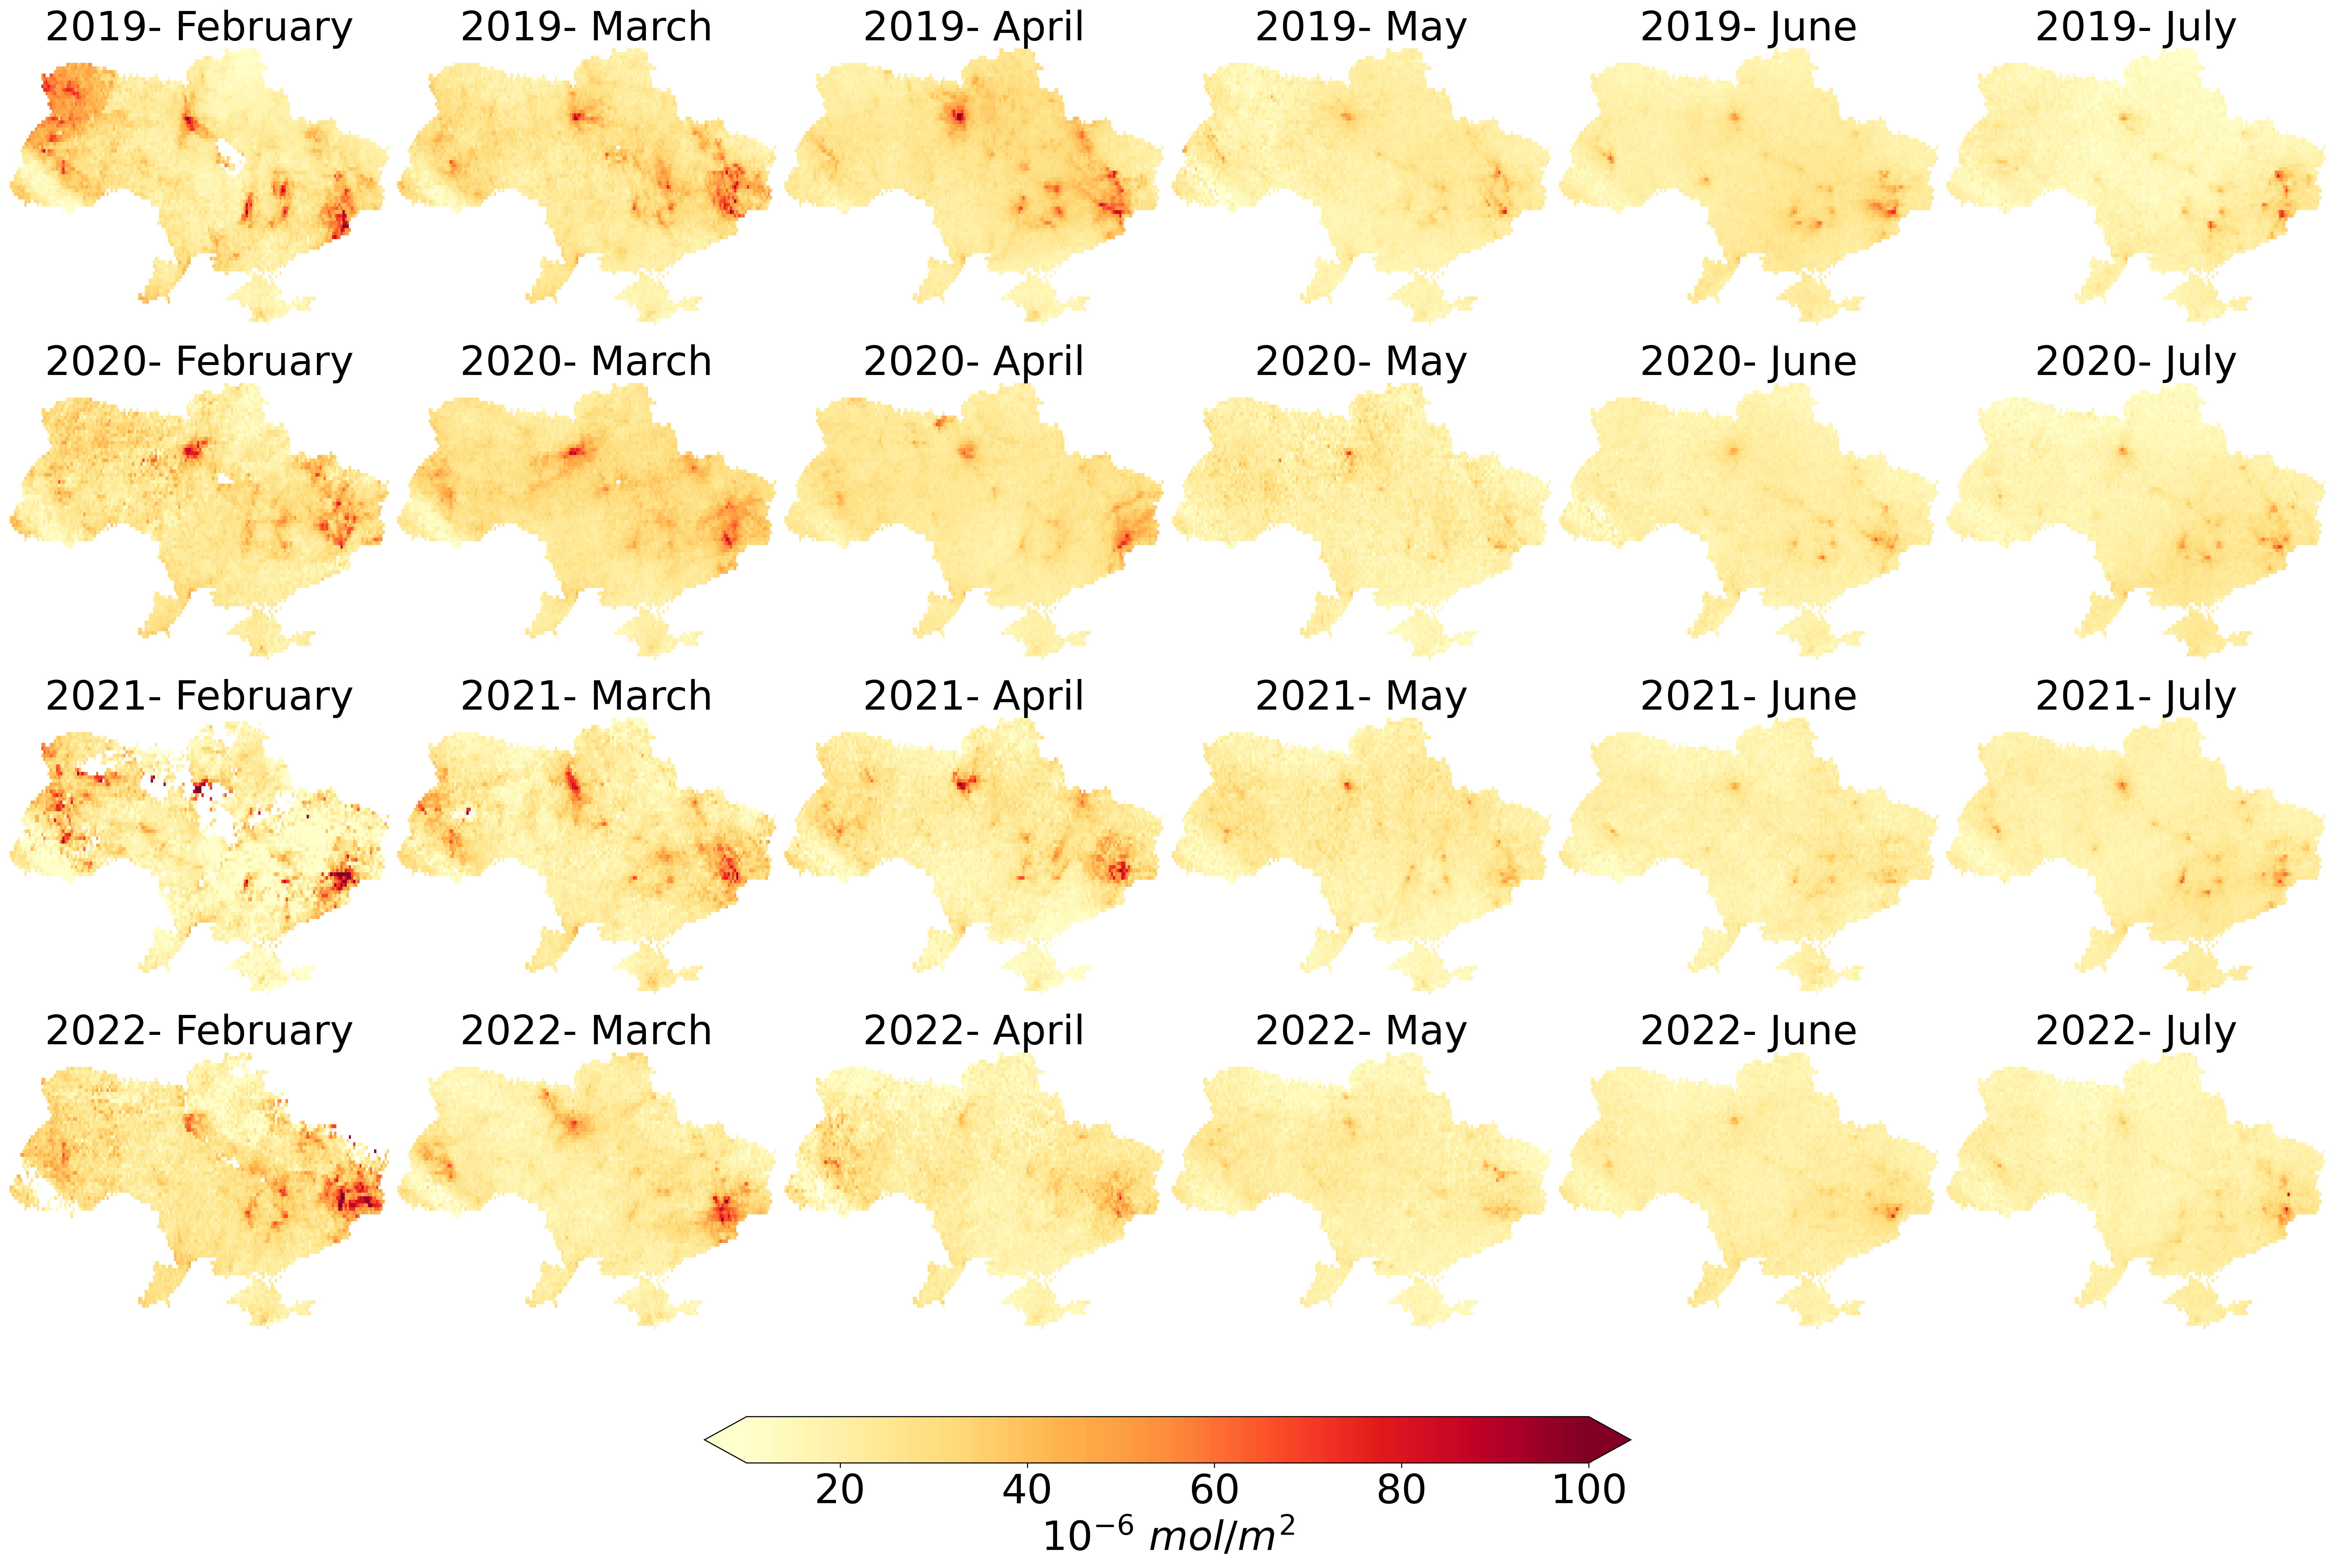
\includegraphics[width=\textwidth]{figs/chap3/fig1_a.png}
      \caption{ORG data}
      \label{fig:chap3_fig1a}
    \end{subfigure}

    \begin{subfigure}{\textwidth}
      \centering
      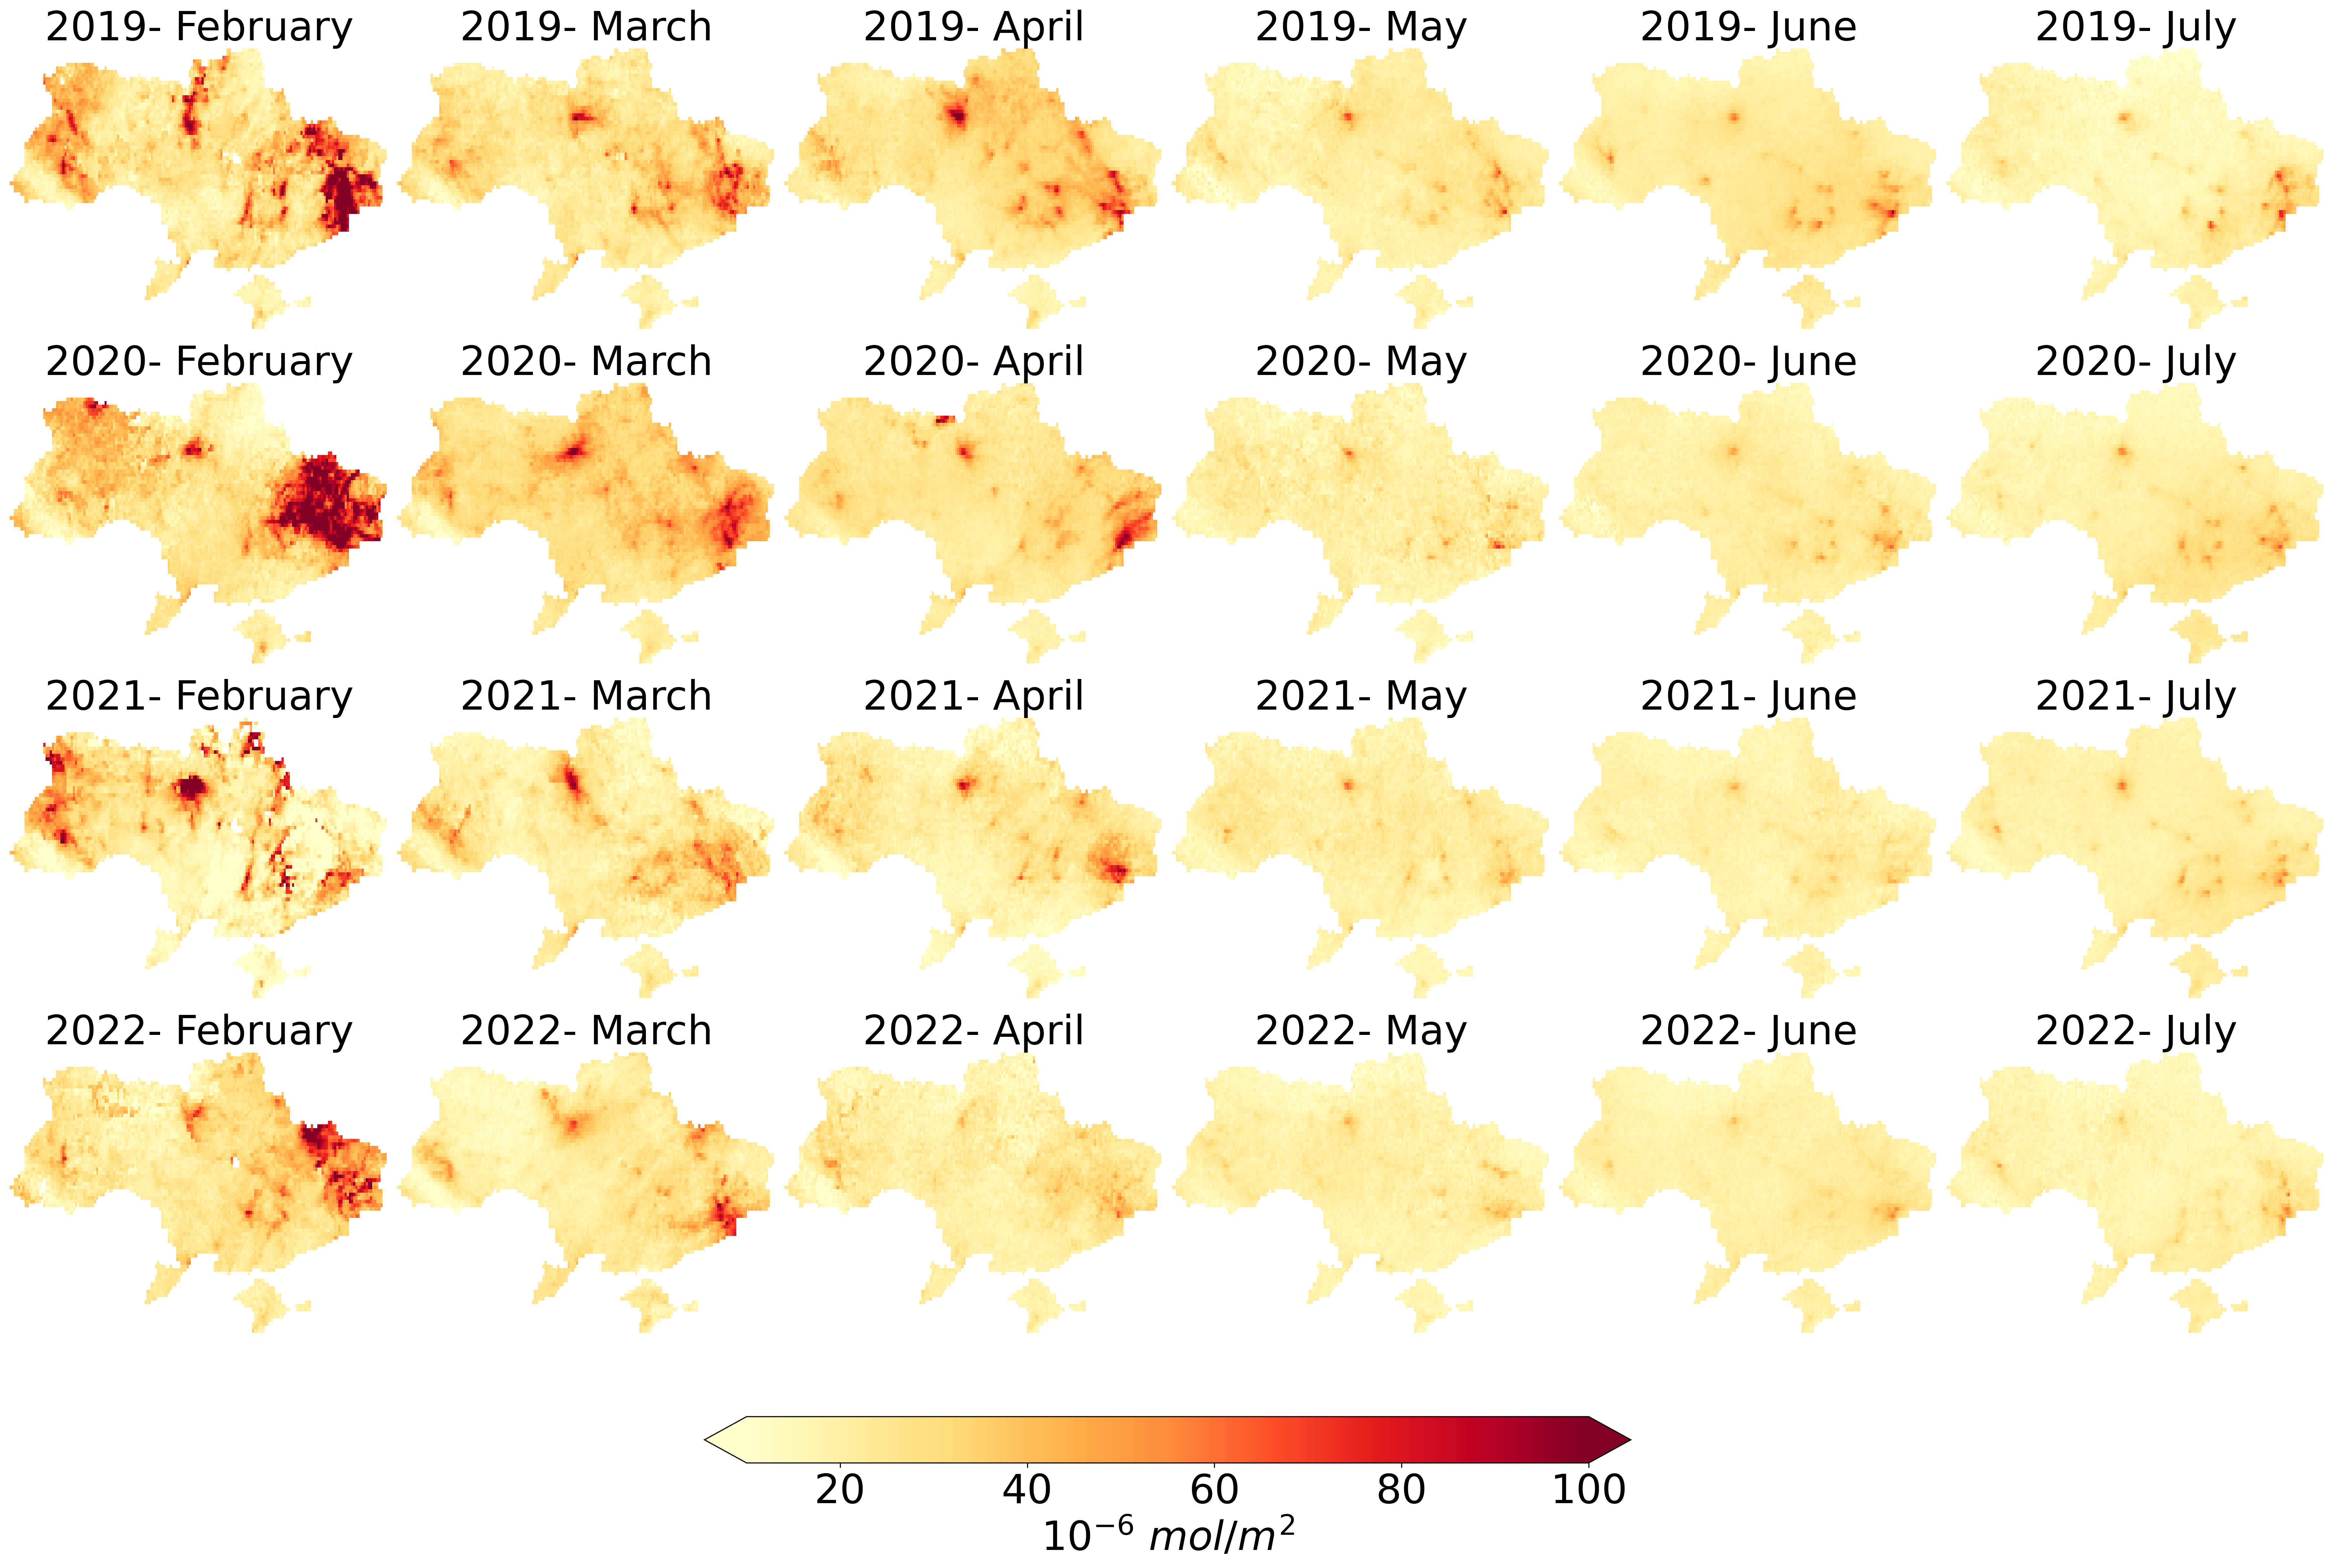
\includegraphics[width=\textwidth]{figs/chap3/fig1_b.png}
      \caption{RPRO data}
      \label{fig:chap3_fig1b}
    \end{subfigure}
    \caption[Monthly map of S5P NO2 in Ukraine]{Monthly (February to July) average map of TROPOMI S5P NO2 tropospheric columns for Ukraine from 2019 to 2022}
    \label{fig:chap3_fig1}
\end{figure}

\begin{figure}[p]
    \centering
    \begin{subfigure}{\textwidth}
      \centering
      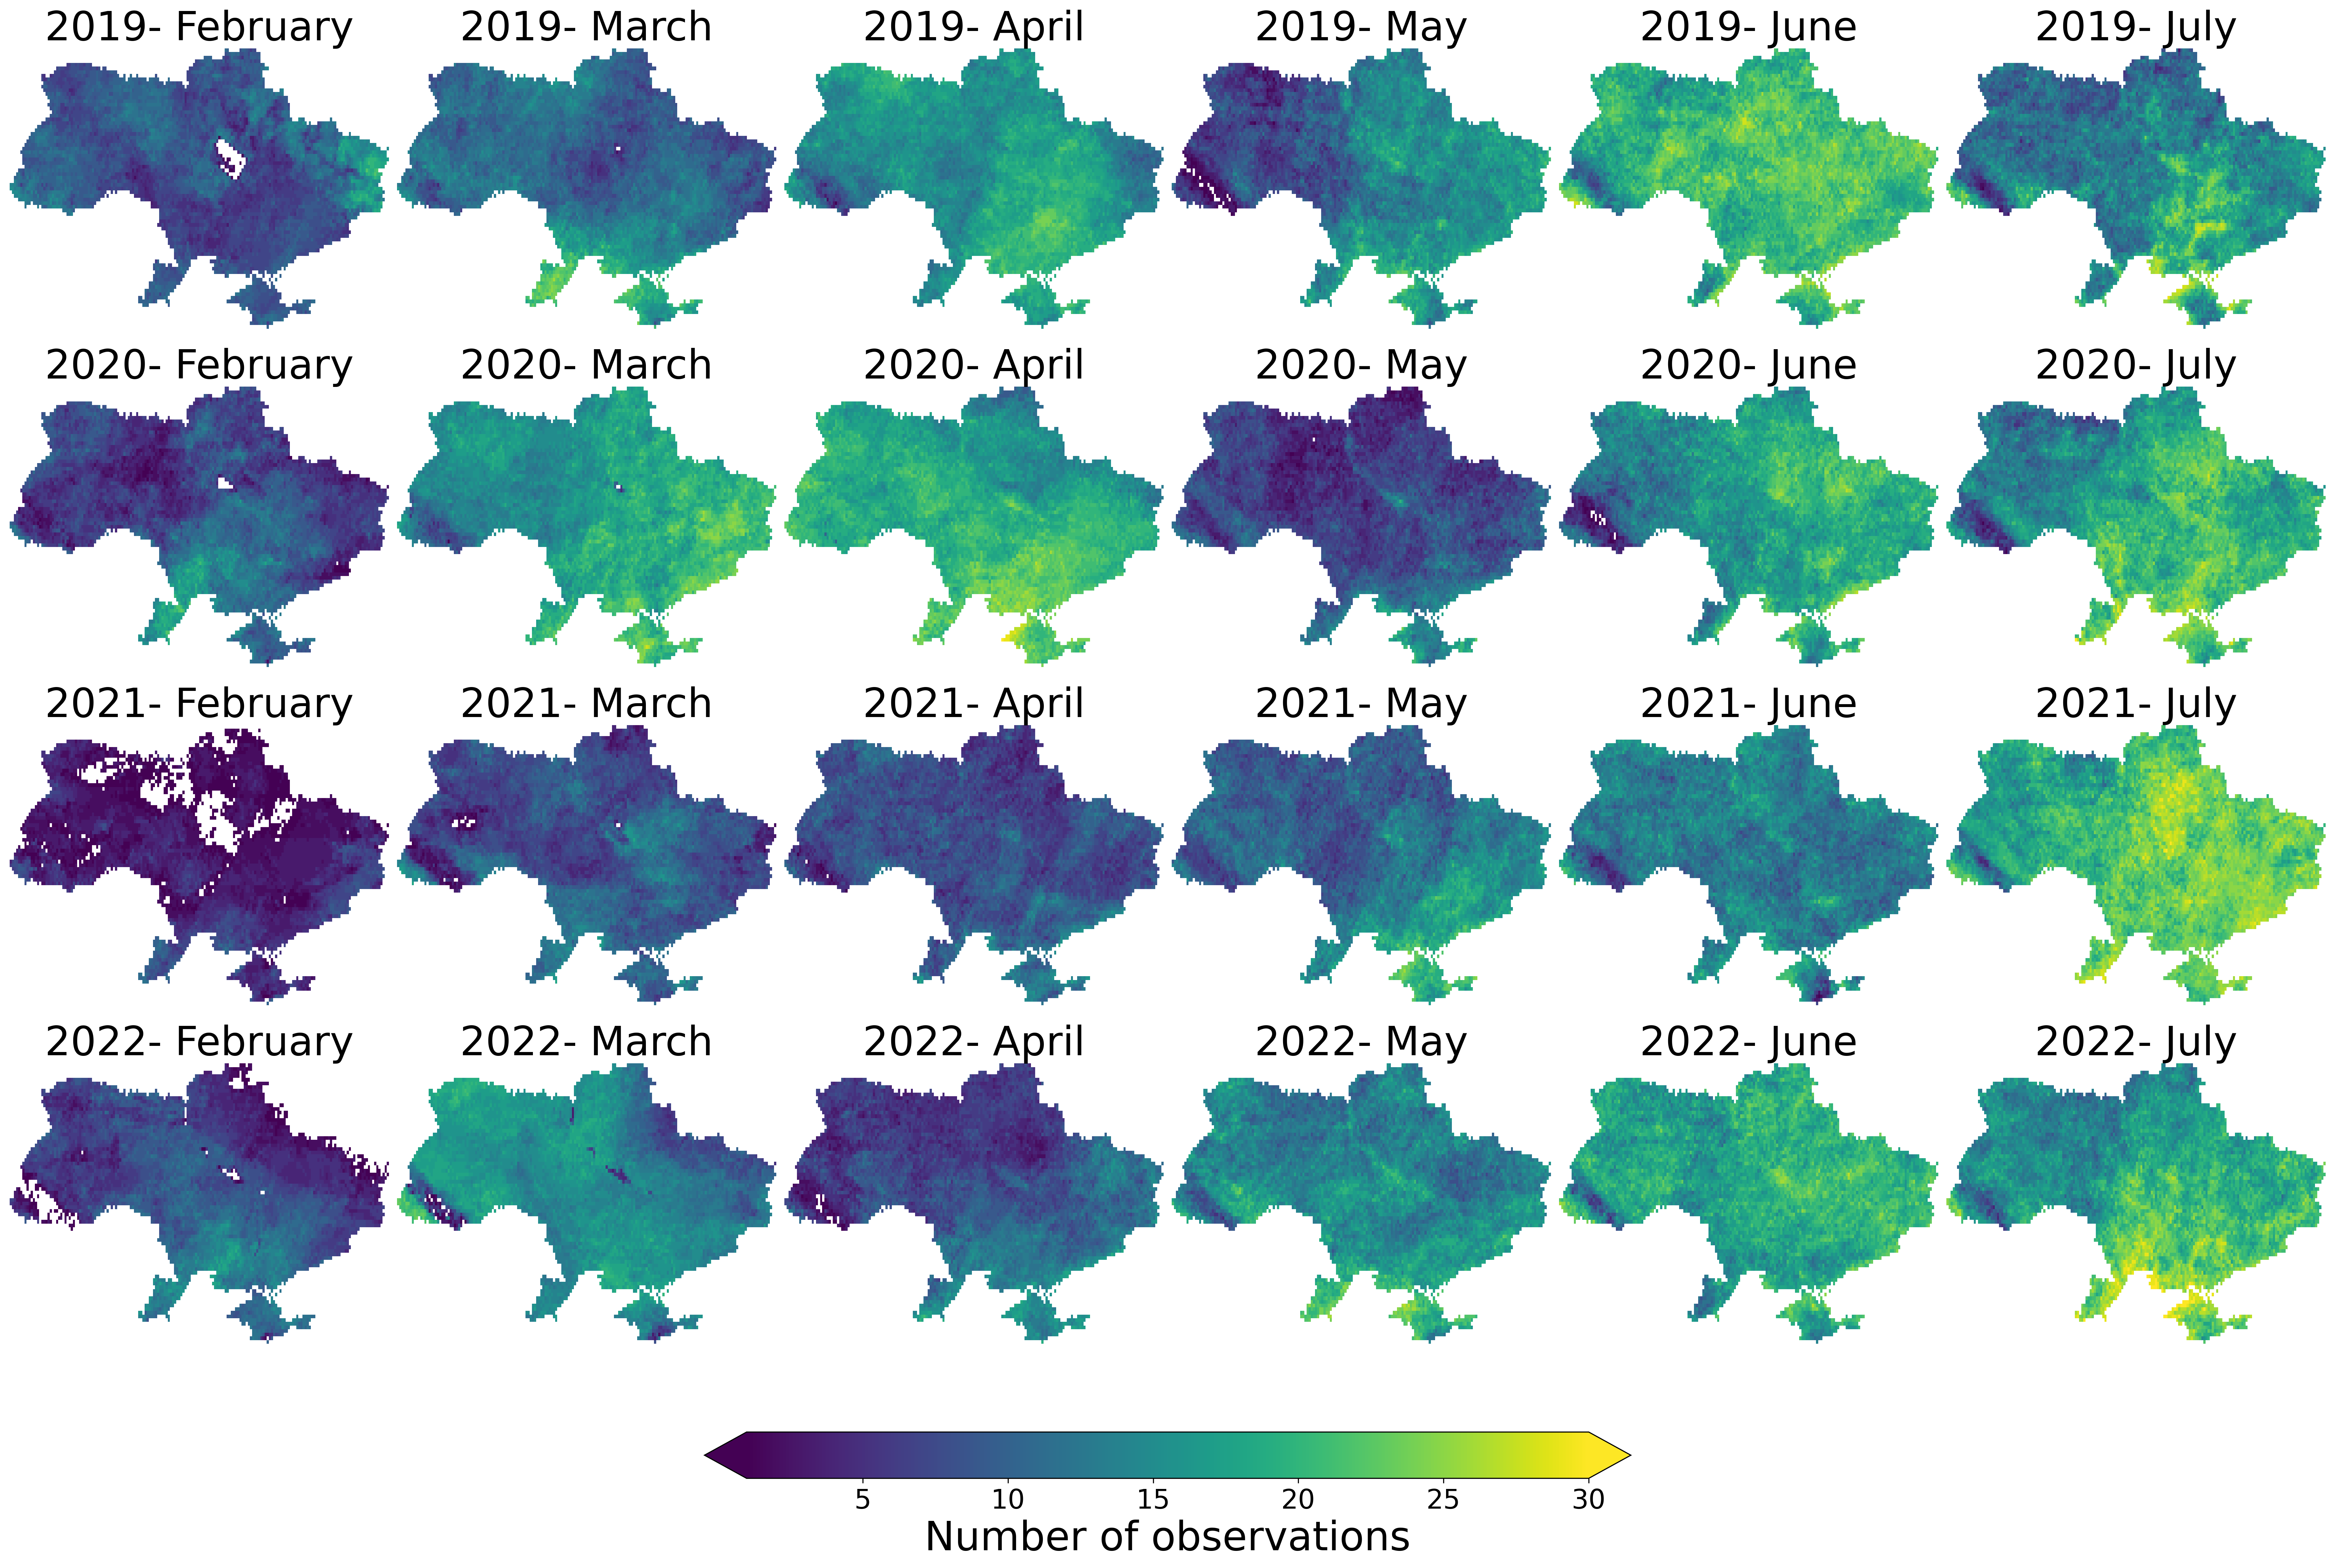
\includegraphics[width=\textwidth]{figs/chap3/fig2_a.png}
      \caption{ORG data}
    \label{fig:chap3_fig2a}
    \end{subfigure}

    \begin{subfigure}{\textwidth}
      \centering
      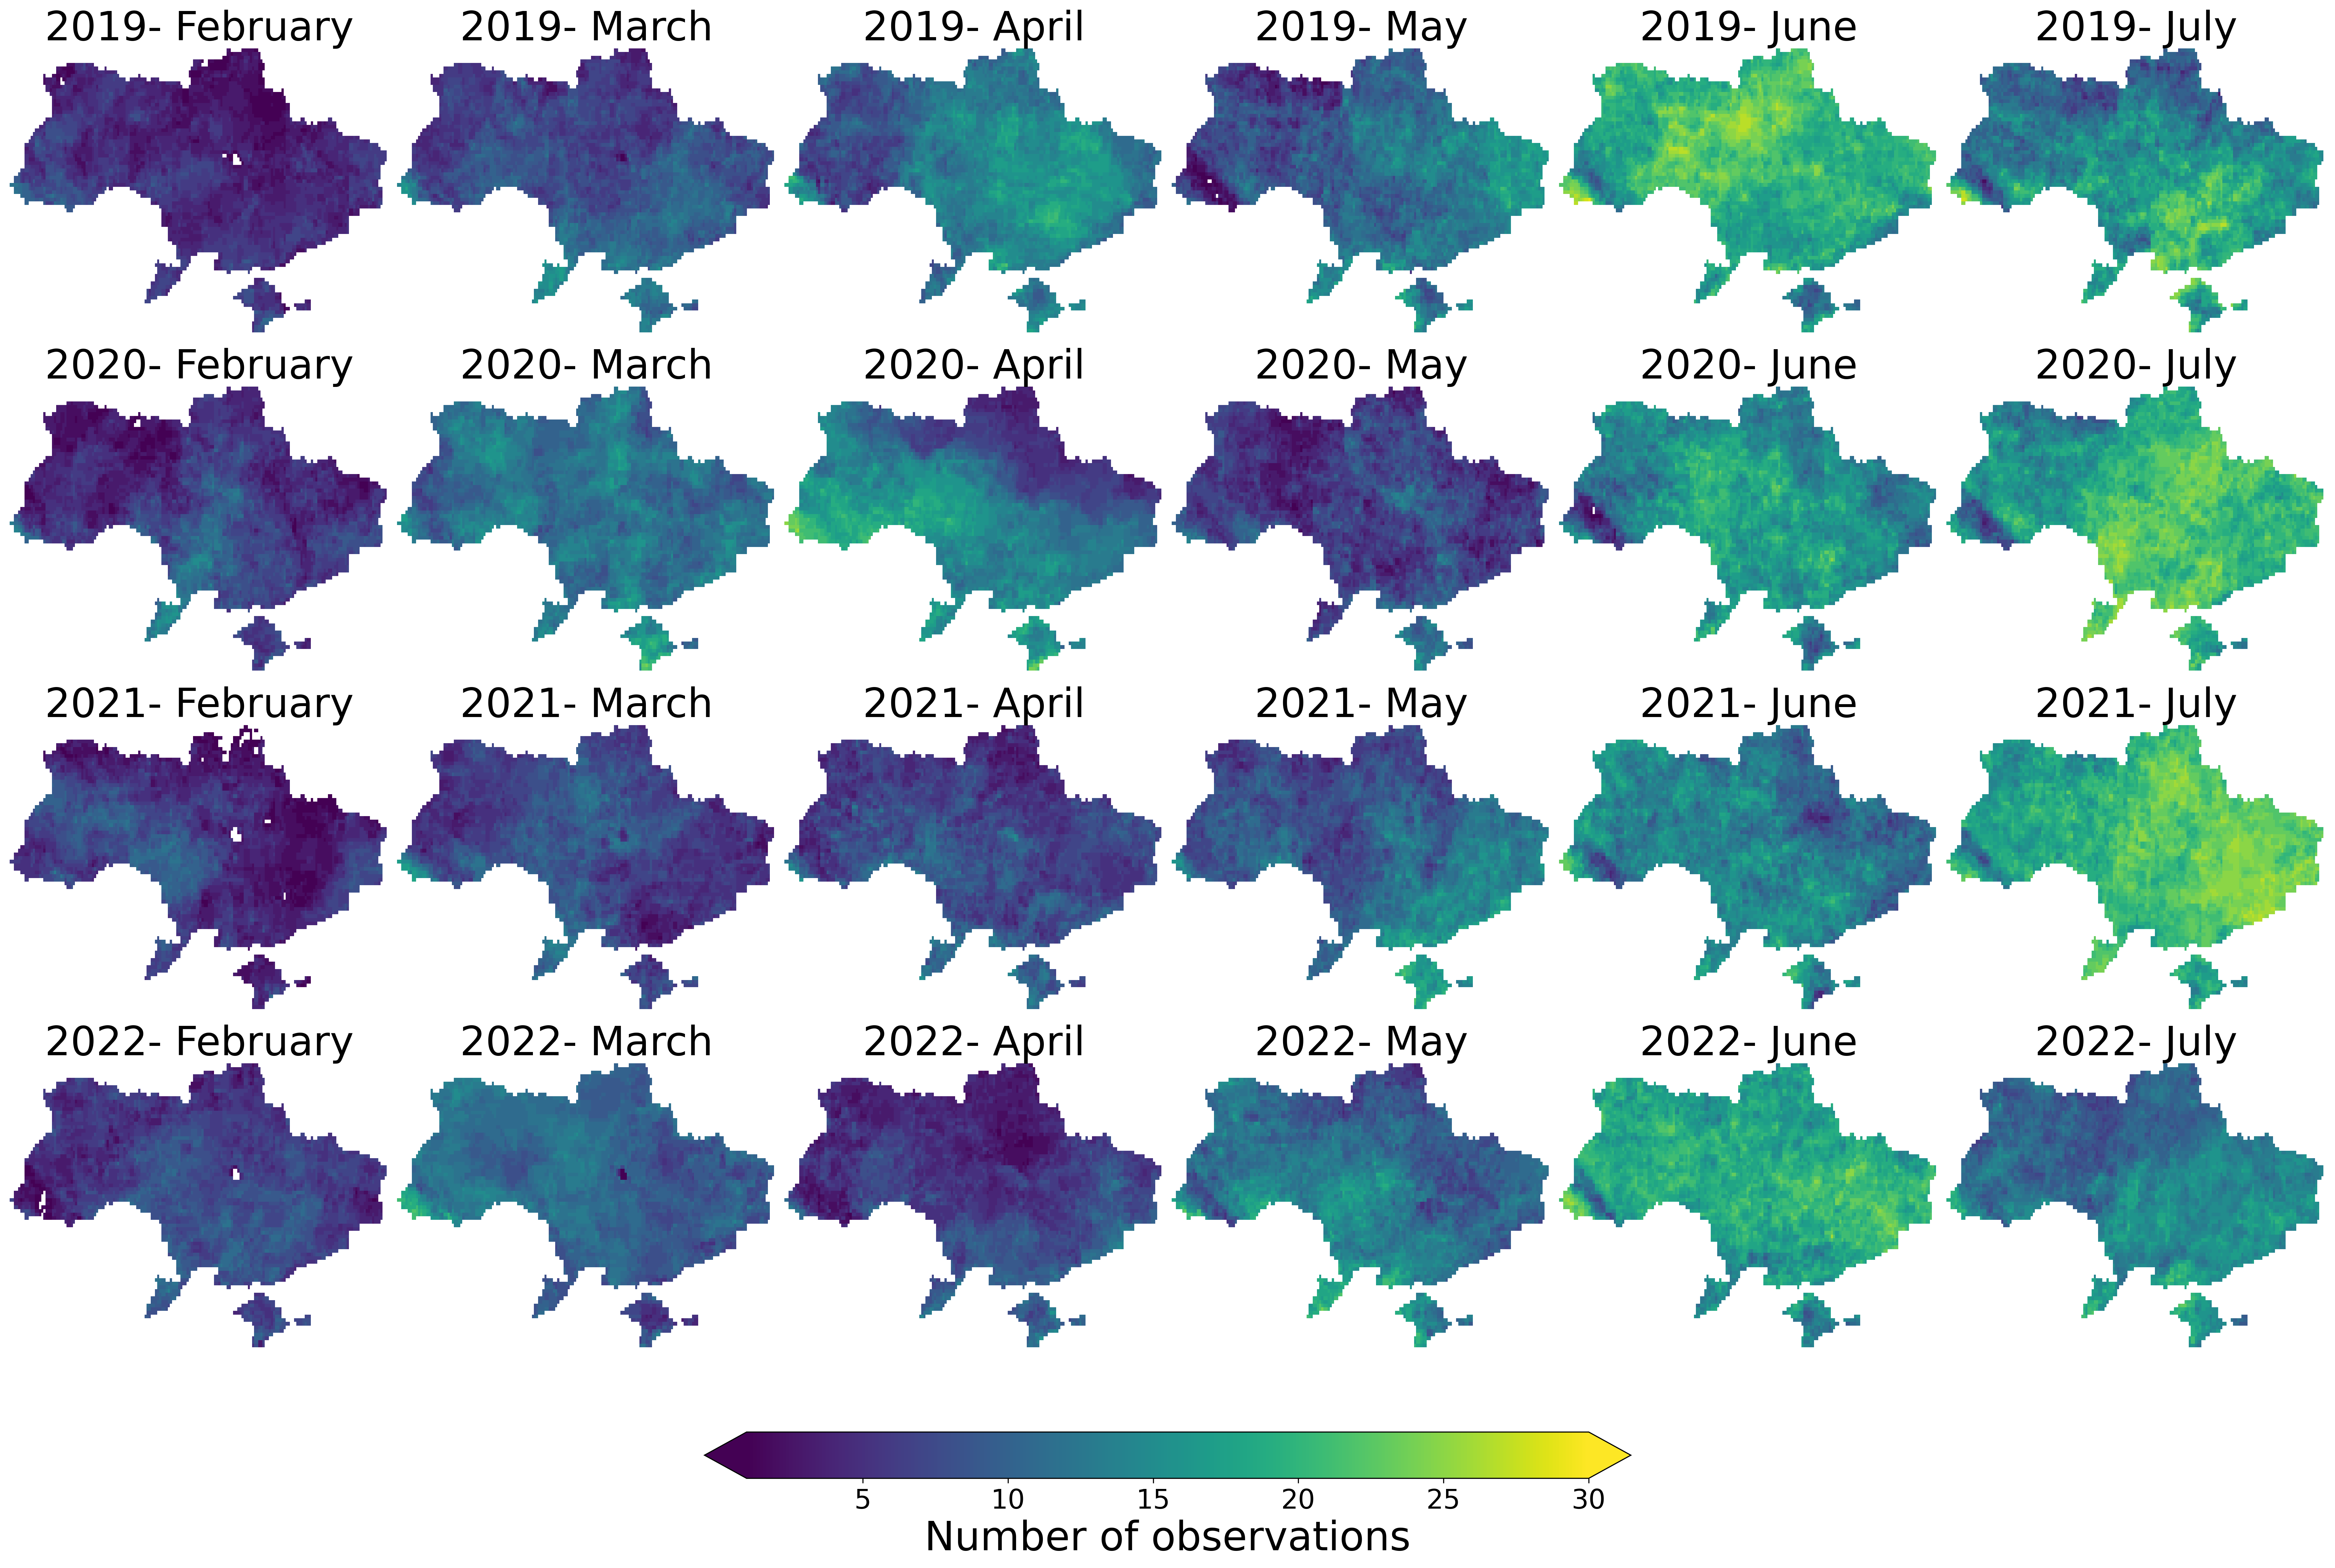
\includegraphics[width=\textwidth]{figs/chap3/fig2_b.png}
      \caption{RPRO data}
      \label{fig:chap3_fig2b}
    \end{subfigure}
    \caption[Monthly number of qualitfied S5P NO2 observations in Ukraine]{Monthly (from February to July) number of TROPOMI S5P NO2 tropospheric columns observations for Ukraine from 2019 to 2022}
    \label{fig:chap3_fig2}
\end{figure}

The S5P data has been distributed from 2018 to the present with two available options. The first is original data (ORG) processed with either of two versions of processor, v1.x (5/2018–6/2021) or v2.x (7/2021 onwards). The second is reprocessed datasets (RPRO) with the processor (v2.x) for the full mission. According to \citep{van2022sentinel}, the S5P NO2 v2.2 data has larger vertical column density (VCDs) than v1.x data, ranging from 10\% to 40\%, mostly found at mid and high latitudes in winter. Therefore, bias between S5P v1.x and v2.x could lead to overestimation and underestimation when comparing air pollution data in 2022 versus 2019, thereby affecting evaluations of the conflict’s impacts on S5P NO2 levels.\par

In this study, we conducted experiments using two versions of S5P NO2 data. The first dataset is ORG data which was collected through level 3 (L3) offline processing (OFF) of the S5P product available on Google Earth Engine \citep{gorelick2017google}. This dataset comprises processed data from different processor versions for each year from 2019 to 2022 (v1.3.1 in 2019, v1.3.2 in 2020, and v2.3.1 in 2022). The second dataset, denoted as the RPRO product, employs processor version v2.4.0 for the full mission duration. This dataset was acquired from the Sentinel-5P Pre-Operations Data Hub (s5phub.copernicus.eu) using the Sentinelsat API.\par

Regarding the RPRO data, we began by downloading the level 2 (L2) dataset. In order to generate the L3 NO2 dataset, each operational L2 product underwent mosaicking and filtering of low-quality pixels, which involved removing items with quality assurance (QA) values less than 75\% for the \enquote{tropospheric\_NO2\_column\_number\_density} band. The harpconvert tool was utilized to perform the conversion from L2 to L3 product. Subsequently, both datasets were linearly interpolated to a spatial resolution of 0.1$\times$0.1 degree. At the time of the experiment, the RPRO data was only accessible until July 2022.\par

Plots presented in Figure \ref{fig:chap3_fig1} display the average monthly TROPOMI NO2 tropospheric column over Ukraine from 2019 to 2022 (February to July) using the ORG data (Figure \ref{fig:chap3_fig1a}) and RPRO data (Figure \ref{fig:chap3_fig1b}), respectively. In 2020, a reduction of 4.8\% (ORG data) and 8.3\% (RPRO data) in mean NO2 levels over the Ukrainian territory was observed from April to May, compared to levels recorded in 2019. In 2022, a reduction of 2.4\% (ORG data) and 2.9\% (RPRO data) was seen from March to July, compared to levels recorded in 2021. Additionally, during the same period, a reduction of 10.3\% (ORG data) and 15\% (RPRO data) was observed, compared to the NO2 levels recorded in 2019. We observed that the reduction in NO2 levels was more significant in the RPRO data compared to the ORG data, both during the lockdown in 2020 and the first five months (March–July) of the conflict in 2022 in Ukraine.\par

We summarize the number of qualified observations available for each month from 2019 to 2022 (February to July) in Ukraine using the ORG data (Figure \ref{fig:chap3_fig2a}) and RPRO data (Figure \ref{fig:chap3_fig2b}). The quantification of seasonal NO2 levels can be challenging, particularly during the selected months in winter (February) and spring (March, April) of 2021 and 2022, due to the limited availability of qualified observations. This is further complicated when attempting to estimate changes before and after intervention events such as the lockdown and the armed conflict in Ukraine, as the before period falls within the winter months when observations are scarce.\par

\subsection{Meteorological and surface NO2 data}
In this study, the meteorological and surface NO2 data are utilized as the predictors for the estimation of NO2 under BAU conditions as suggested by \citep{barre2021estimating}. The meteorological data is ERA5 reanalysis data which is collected from the Climate Data Store of the Copernicus Climate Change Service \citep{hersbach2018era5}. We use the following weather variables: 10 m wind speed  (u and v component, m/s) and direction (degrees), 2m air temperature (K), 2m dewpoint temperature (K), relative humidity (\%), geopotential (m2/s2), and BLH (m). All the variables are downloaded at the original resolution of 0.25$\times$0.25 degree and then linearly interpolated to 0.1$\times$0.1 degree (about 10km$\times$10km) resolution. The utilized surface NO2 data is collected from CAMS European air quality forecast and reanalyses and forecast \citep{marecal2015regional} by using the Atmosphere Data Store of the CAMS (https://ads.atmosphere.copernicus.eu/). Since the forecast data is a 3-year rolling archive from the present, we utilized the analysis data for 2019. The surface NO2 forecast data served as the predictors under the BAU scenario for 2020 to 2022. As forecast predictions do not involve an assimilation process \citep{barre2021estimating}, we expect no effect of the pandemic lockdown, and the impact of the armed conflict related events on air pollution was included in the surface NO2 pollution level. Both forecast and analysis data are available at the resolution of 0.1$\times$0.1 degree. We calculated the mean values based on data from 13:00 and 14:00hours local time to represent the surface NO2 and meteorology value at the time the satellite S5P overpassed Ukraine. \par
\subsection{Fire spots database and Ukraine crisis hub}
In order to draw a detailed picture of the battle spots, we utilized data from Fire Information for Resource Management System (FIRMS) provided by National Aeronautics and Space Administration (NASA) and Ukraine Crisis Hub data from the Armed Conflict Location and Event Data Project (ACLED) \citep{raleigh2010introducing}. The NASA FIRMS portal provides active fire data at three-hour intervals based on satellite observations from products of the Moderate Resolution Imaging Spectroradiometer (MODIS) and Visible Infrared Imaging Radiometer Suite (VIIRS). For the study, data from the VIIRS product was employed to access the active fire spots due to its superior fire detection capabilities compared to the MODIS products \citep{csiszar2014active,schroeder2014new}. \par

Detailed data on conflict hotspot locations are extracted from the Ukraine Crisis Hub which is distributed by ACLED \citep{raleigh2010introducing}. Information regarding the conflict events is updated weekly and disaggregated to event type with time and location (latitude and longitude) in Ukraine and the Black Sea region available from 2018 until the present. As a result of the conflict, we expect to see and identify corresponding patterns between locations of active fire spots and the locations of conflict events. \par
\subsection{Population data}
As NO2 pollution levels are closely related to human socio-economic activities and frequently high in populous urban areas, we downloaded 2020 population data for Ukraine from the WorldPop Global Project (www.worldpop.org), available annually at the spatial resolution of 100m$\times$100m as one of the features for the BAU NO2 model. The population data was collected, clipped to the Ukrainian territory, and linearly interpolated to 0.1$\times$0.1 degree (about 10km$\times$10km).\par
\section{Business-as-usual (BAU) modelling} \label{chap3_bau}
When considering changes induced by the pandemic lockdown and the armed conflict, especially for before-after analysis, an important factor is the meteorology variations. In this study, we use a suggested list of predictors by \citep{barre2021estimating}, which consists of meteorological, spatial, and temporal features, population counts from WorldPop Global Project, and surface NO2 pollution levels from CAMS European analysis data for 2019 and forecast data for 2020 to 2022 for BAU model development. The spatial and temporal features contain latitude, longitude, Julian date (number of the day from January 1), and day of the week, respectively. However, unlike the study cited \citep{barre2021estimating}, for machine learning model selection, instead of GBM we utilized LightGBM \citep{ke2017lightgbm}, which is a gradient boosting decision tree, to build the BAU model. During the training process, other than in studies that used the grid search with an n-fold cross-validation approach to tune the model’s hyperparameters \citep{barre2021estimating,petetin2020meteorology}, we employed the Fast Library for Automated Machine Learning (FLAML) \citep{wang2021flaml}, which is a new lightweight library for quickly determining the accurate model, to find the optimum hyperparameters for the LightGBM model in our case. \par
\begin{table}[!ht]
    \centering
    \caption[Model performance evaluation]{The performance of the BAU model on the validation set described using the following metrics: mean bias (MB), normalized mean bias (nMB), root mean square error (RMSE), normalized root mean square error (nRMSE) and Pearson correlation coefficient (R). N represents the number of points in both the training set and validation set, where each point is associated with unique latitude and longitude values. There are no duplicate points shared between the training and validation sets.}
    \begin{tabular}{c c c c c c c}
    \hline
        ~ & MB  & nMB & RMSE & nRMSE & R & n \\ \hline
        \multicolumn{7}{c}{Performance with S5P data version 1.x\textminus ORG data} \\ \hline
        Training set & $\mathrm{3.68}\times10\textsuperscript{-5}$ & $\mathrm{1.53}\times10\textsuperscript{-4}$ & 7.80 & 7.40 & 0.87 & 5022  \\
        Validation set & 0.03 & 0.10 & 9.53 & 10.98 & 0.80 & 1269 \\ \hline
        \multicolumn{7}{c}{Performance with S5P data version 2.4\textminus RPRO data} \\ \hline
        Training set & $\mathrm{2.67}\times10\textsuperscript{-4}$ & $\mathrm{1.04}\times10\textsuperscript{-3}$ & 6.97 & 5.12 & 0.91 & 5051  \\
        Validation set & 0.07 & 0.26 & 8.47 & 7.75 & 0.86 & 1242 \\ \hline
    \end{tabular}
    \label{tab:chap3_tab1}
\end{table}

\begin{figure}[tbh!]
    \centering
    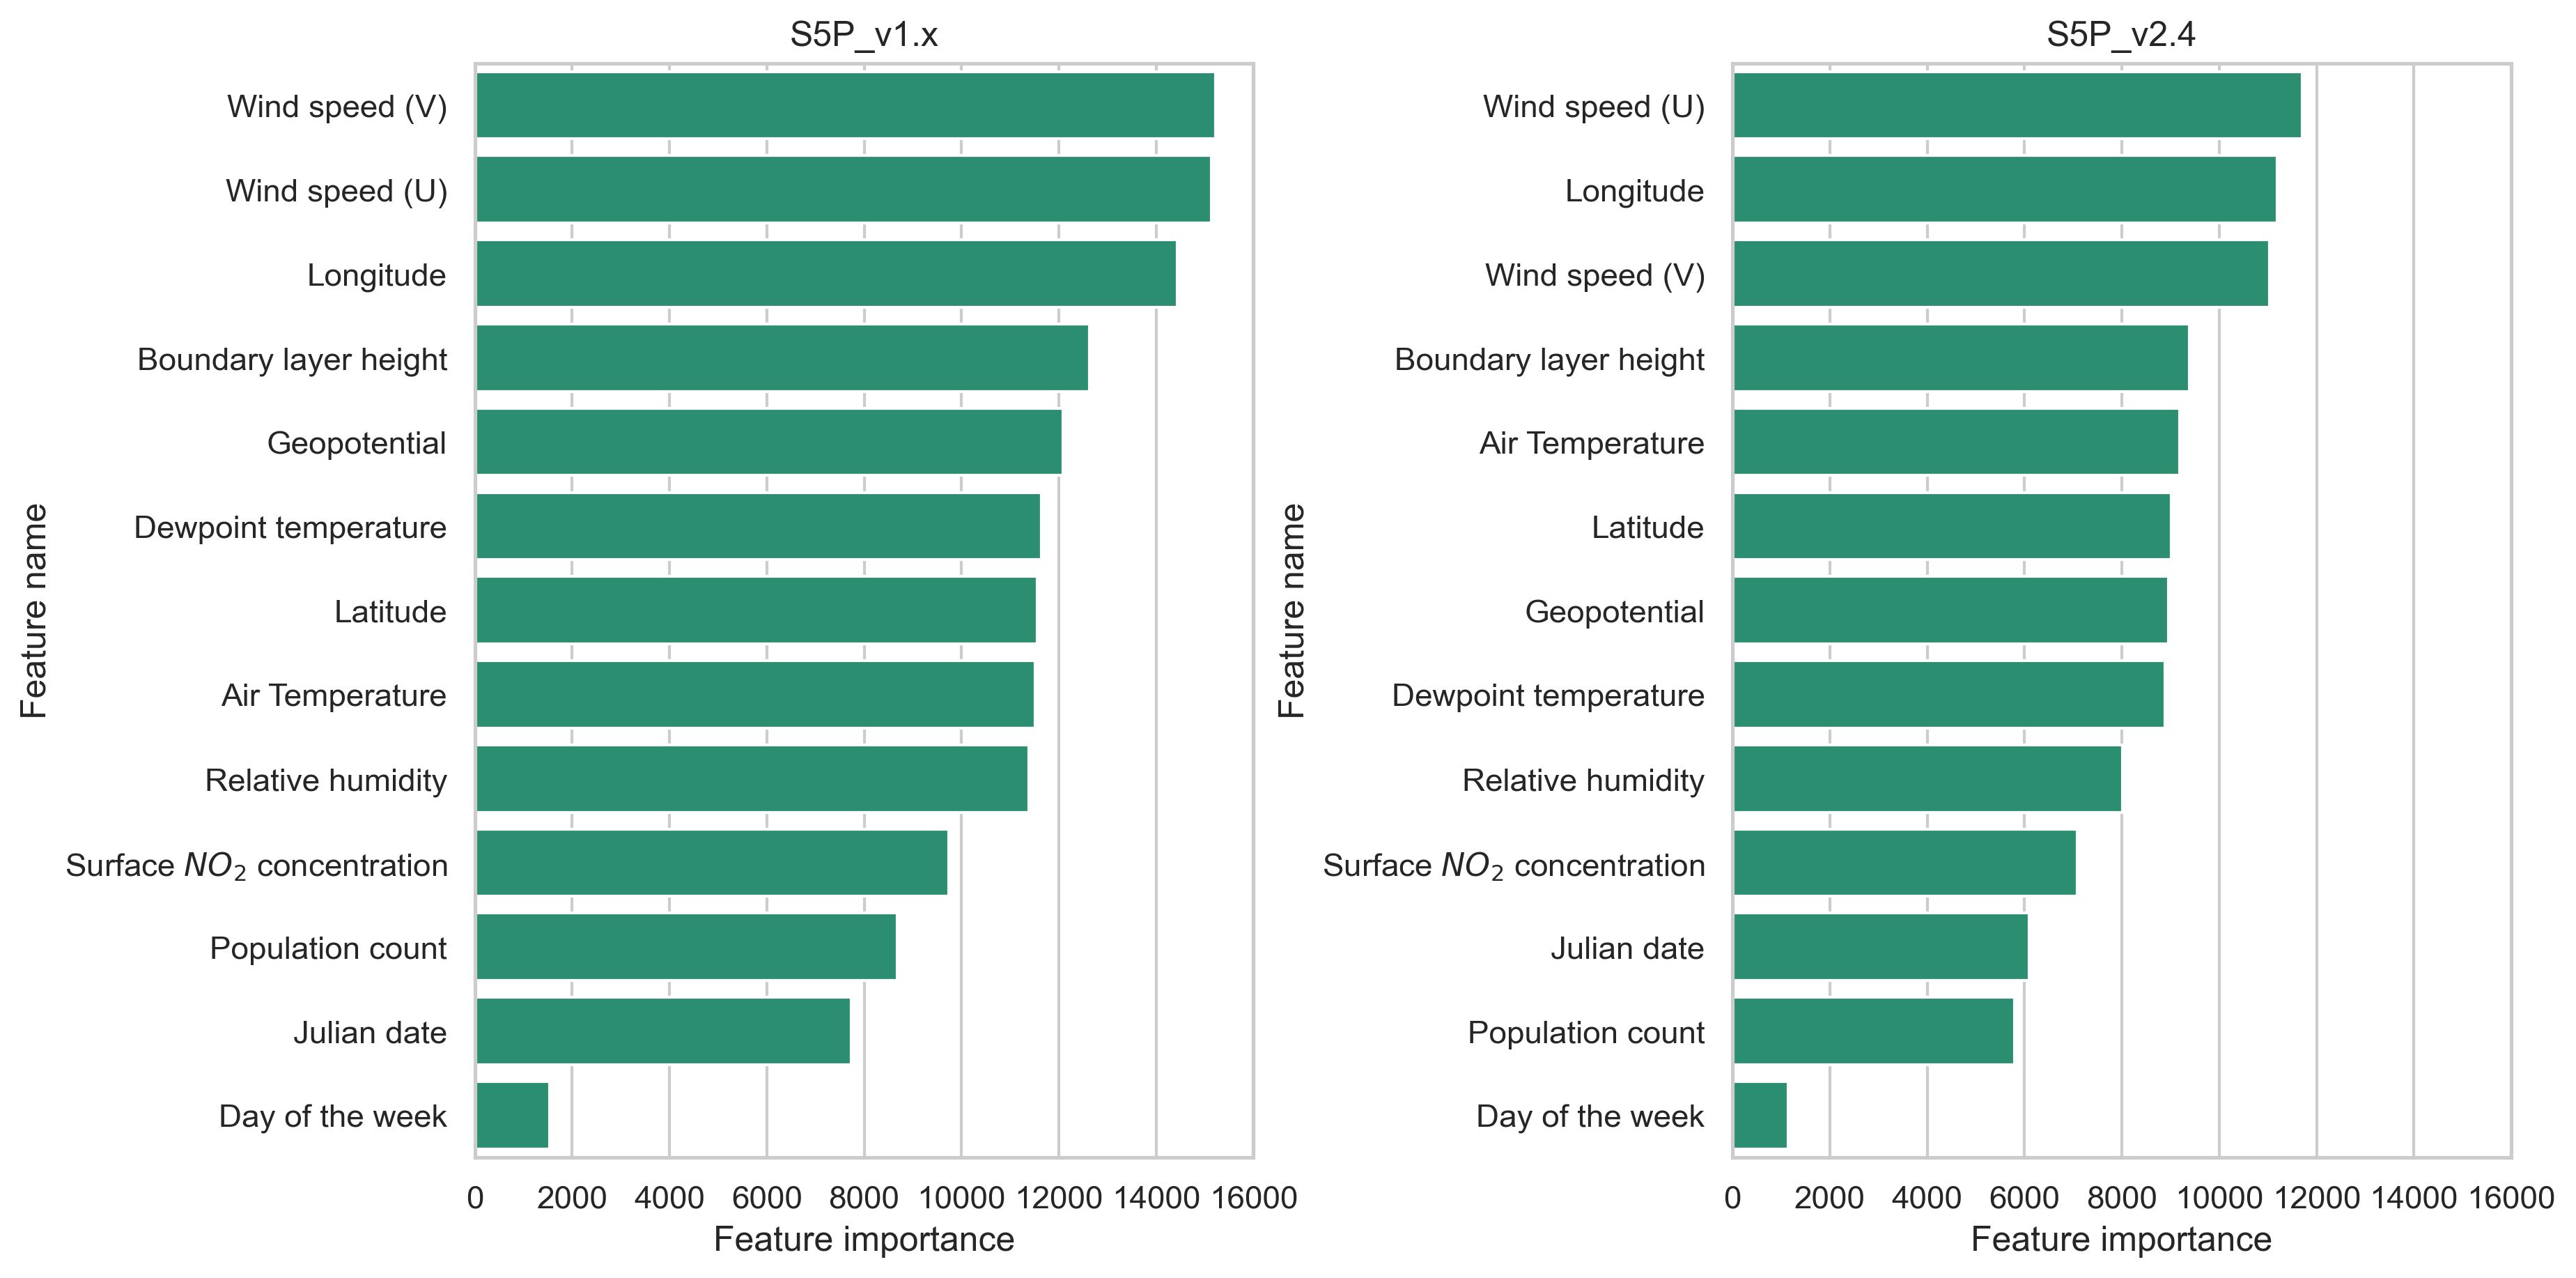
\includegraphics[width=\textwidth]{figs/chap3/figA1.png}
    \caption{Feature importance estimated using LightGBM split method.}
    \label{fig:chap3_figa1}
\end{figure}

\begin{figure}[tbh!]
    \centering
    \begin{subfigure}{\textwidth}
      \centering
      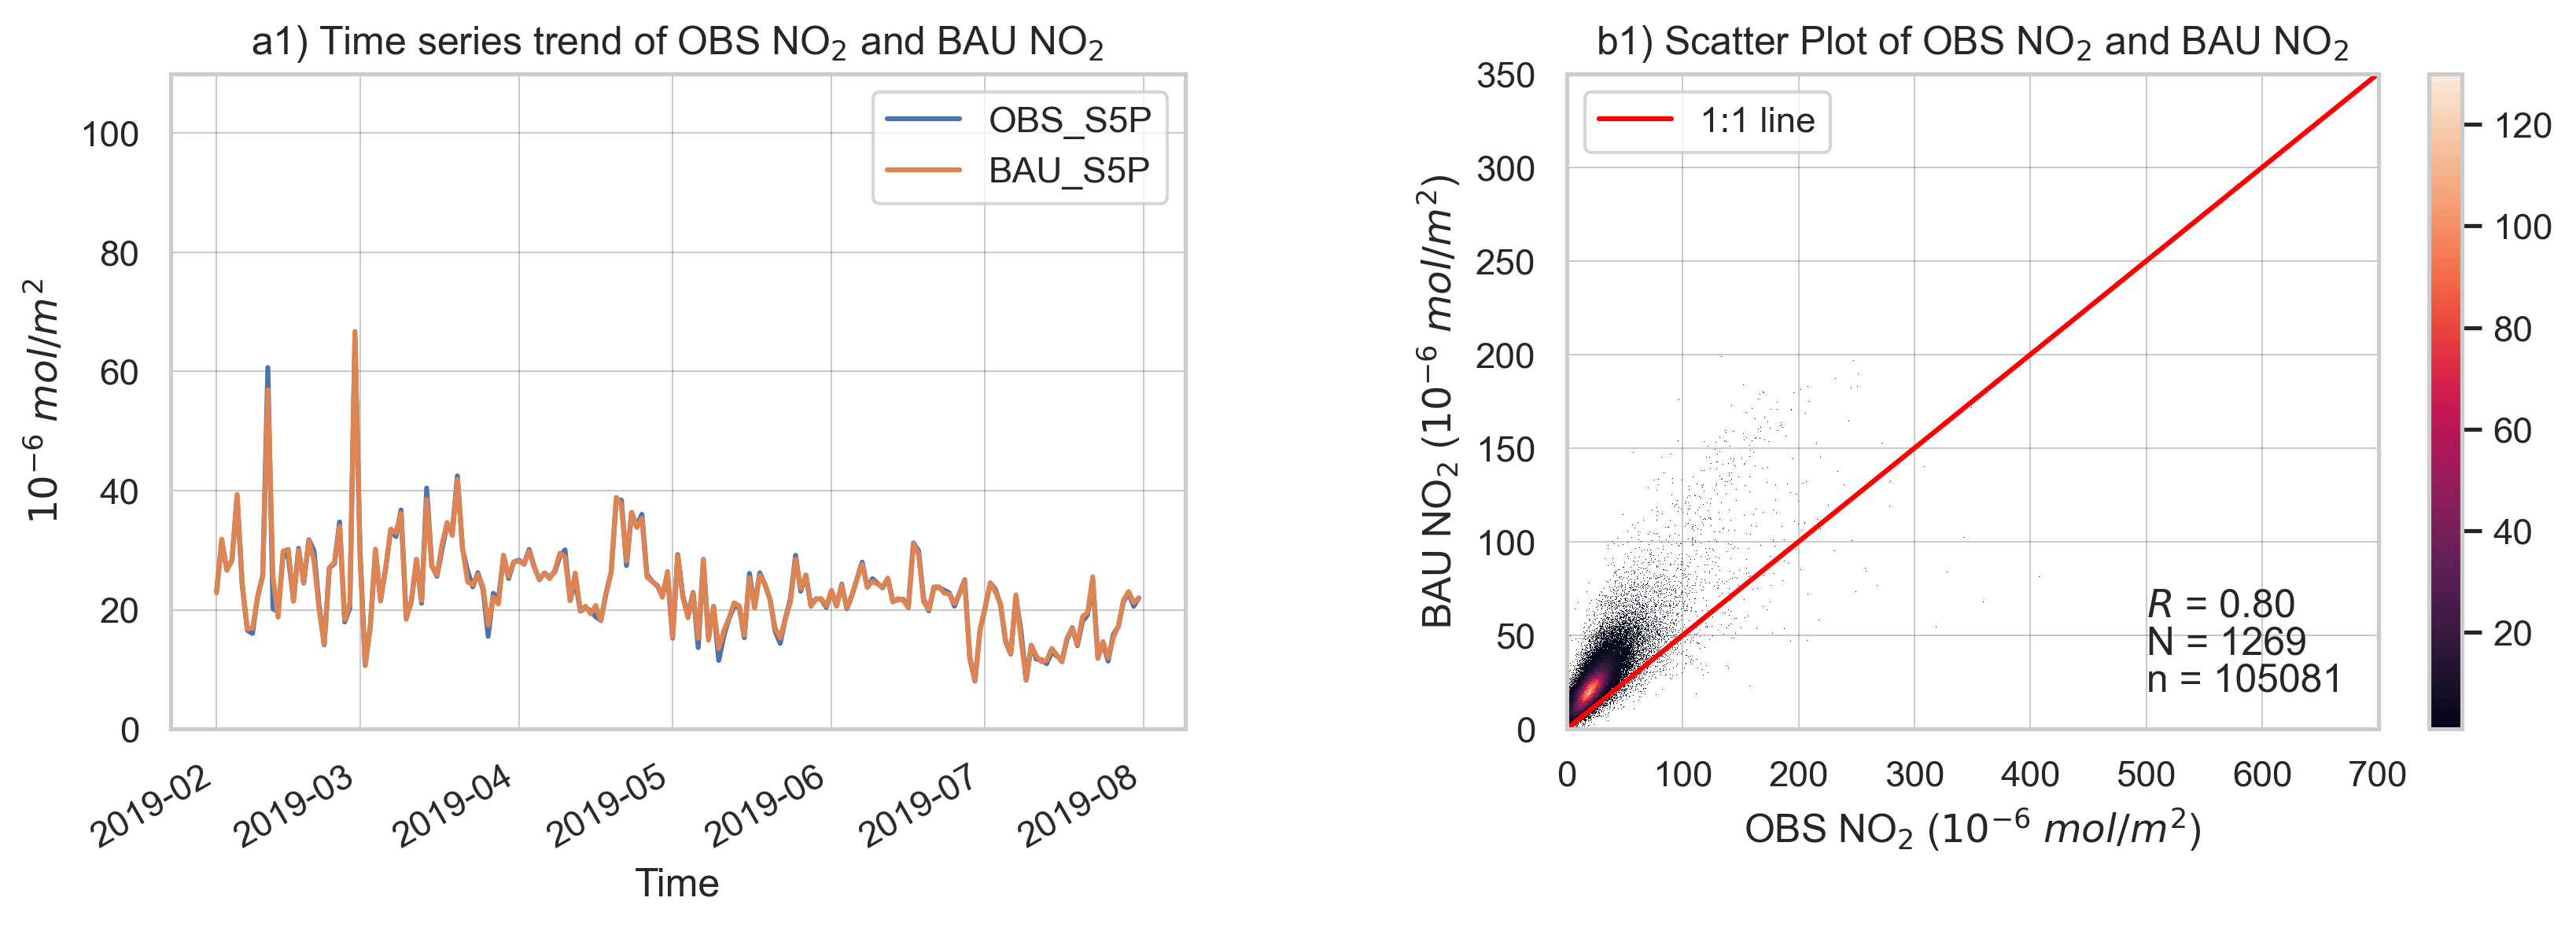
\includegraphics[width=\textwidth]{figs/chap3/figA2-a1b1.png}
    \end{subfigure}

    \begin{subfigure}{\textwidth}
      \centering
      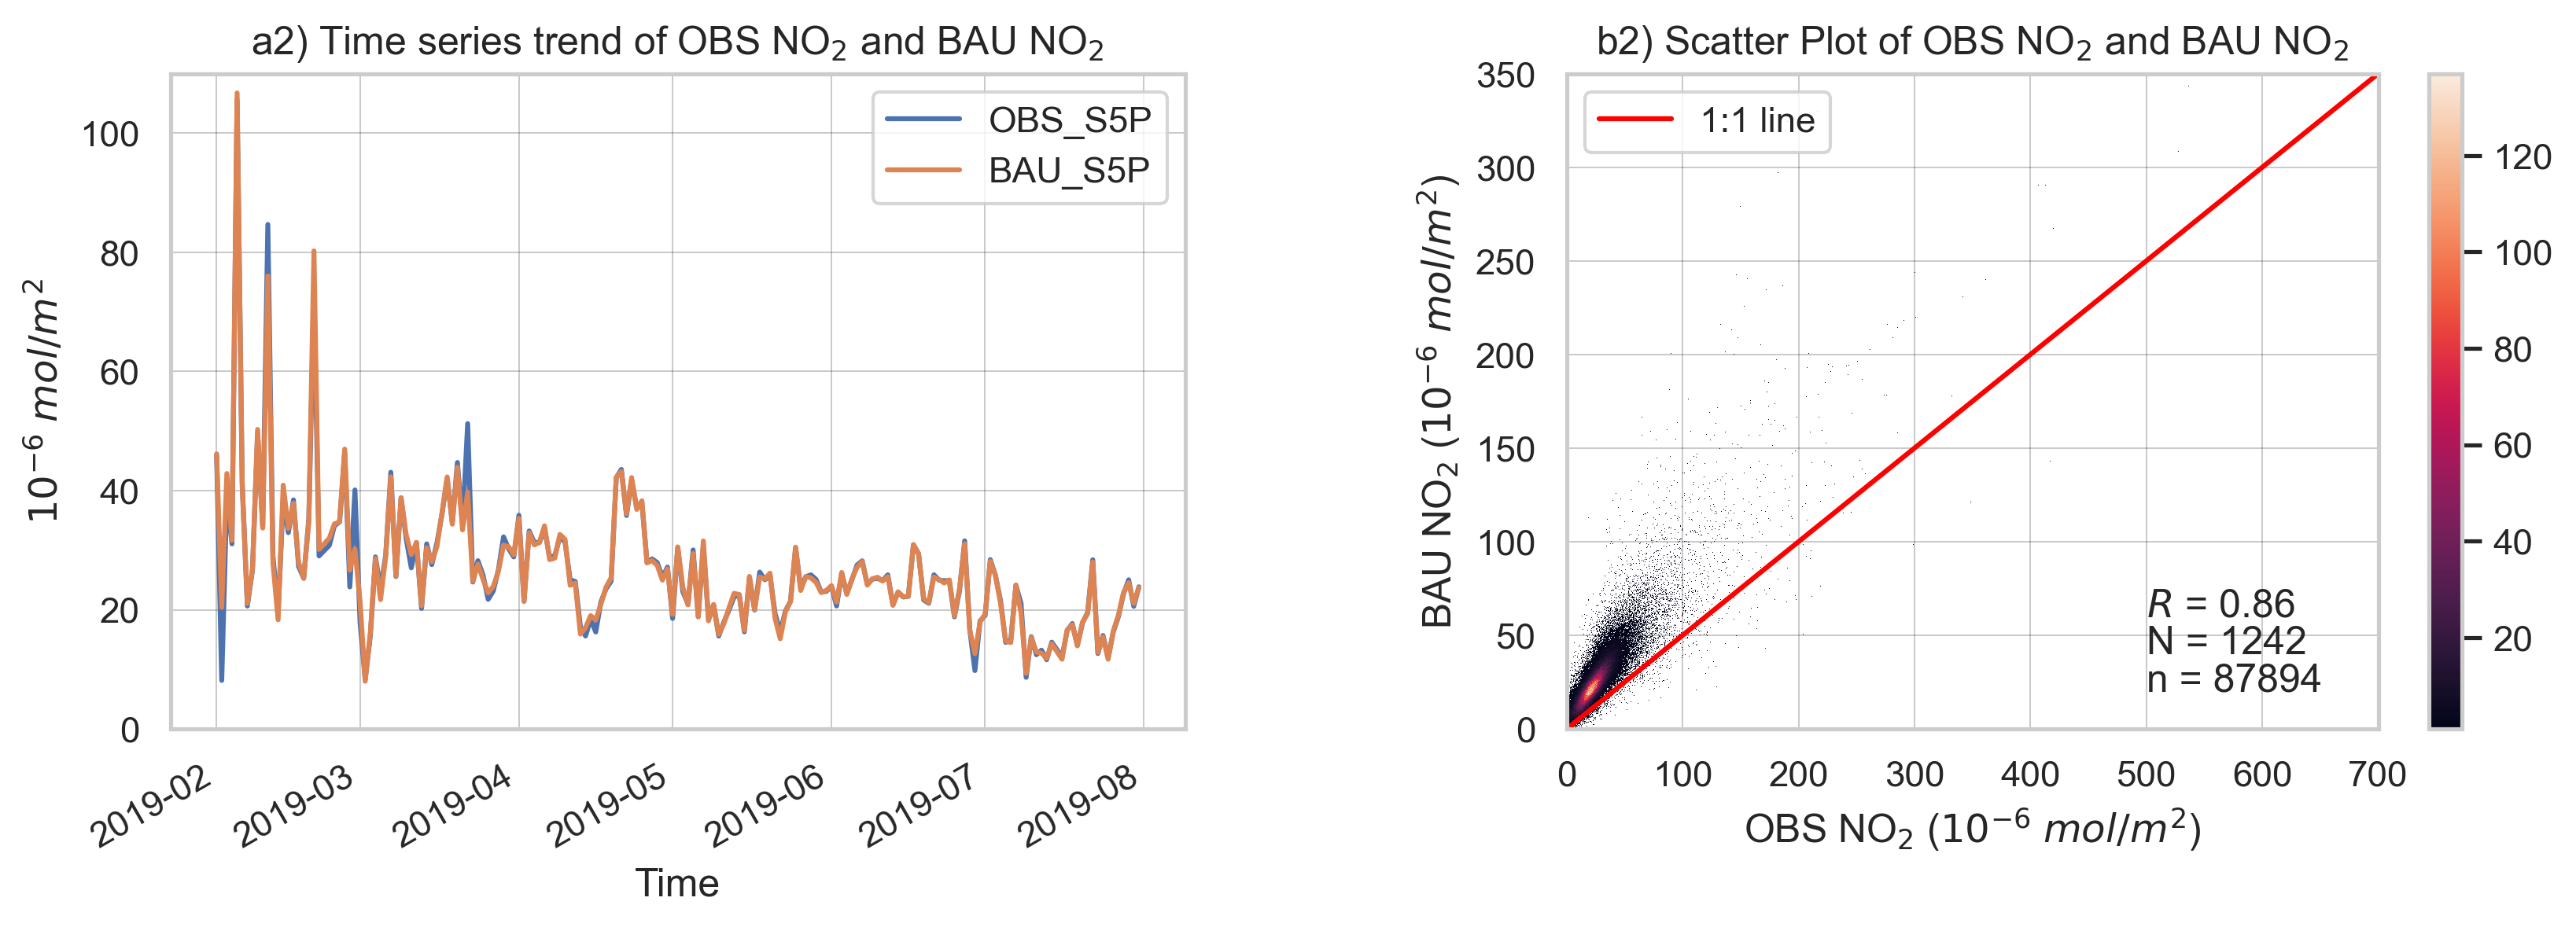
\includegraphics[width=\textwidth]{figs/chap3/figA2-a2b2.png}
    \end{subfigure}
    \caption[Model performance evaluation]{The timeseries trend lines (a1) and (a2) and scatter plots (b1) and (b2) depict the OBS NO2 and BAU NO2 on the validation set in 2019. Sub-figures (a1) and (b1) correspond tothe S5P version 1.x data, while sub-figures (a2) and (b2) represent the S5P version 2.4 data. Inthe scatter plot, we showed the 1:1 line, Pearson correlation coefficient (R), N represents thenumber of points in both the training set and validation set, where each point is associated withunique latitude and longitude values. At each point, we used the available daily data fromFebruary 1 to July 31, 2019, to make the training and validation set with total number samples isdenoted as  n. There are no duplicate points and samples shared between the training andvalidation sets.}
    \label{fig:chap3_figa2}
\end{figure}


\begin{figure}[p]
    \centering
    \begin{subfigure}{\textwidth}
      \centering
      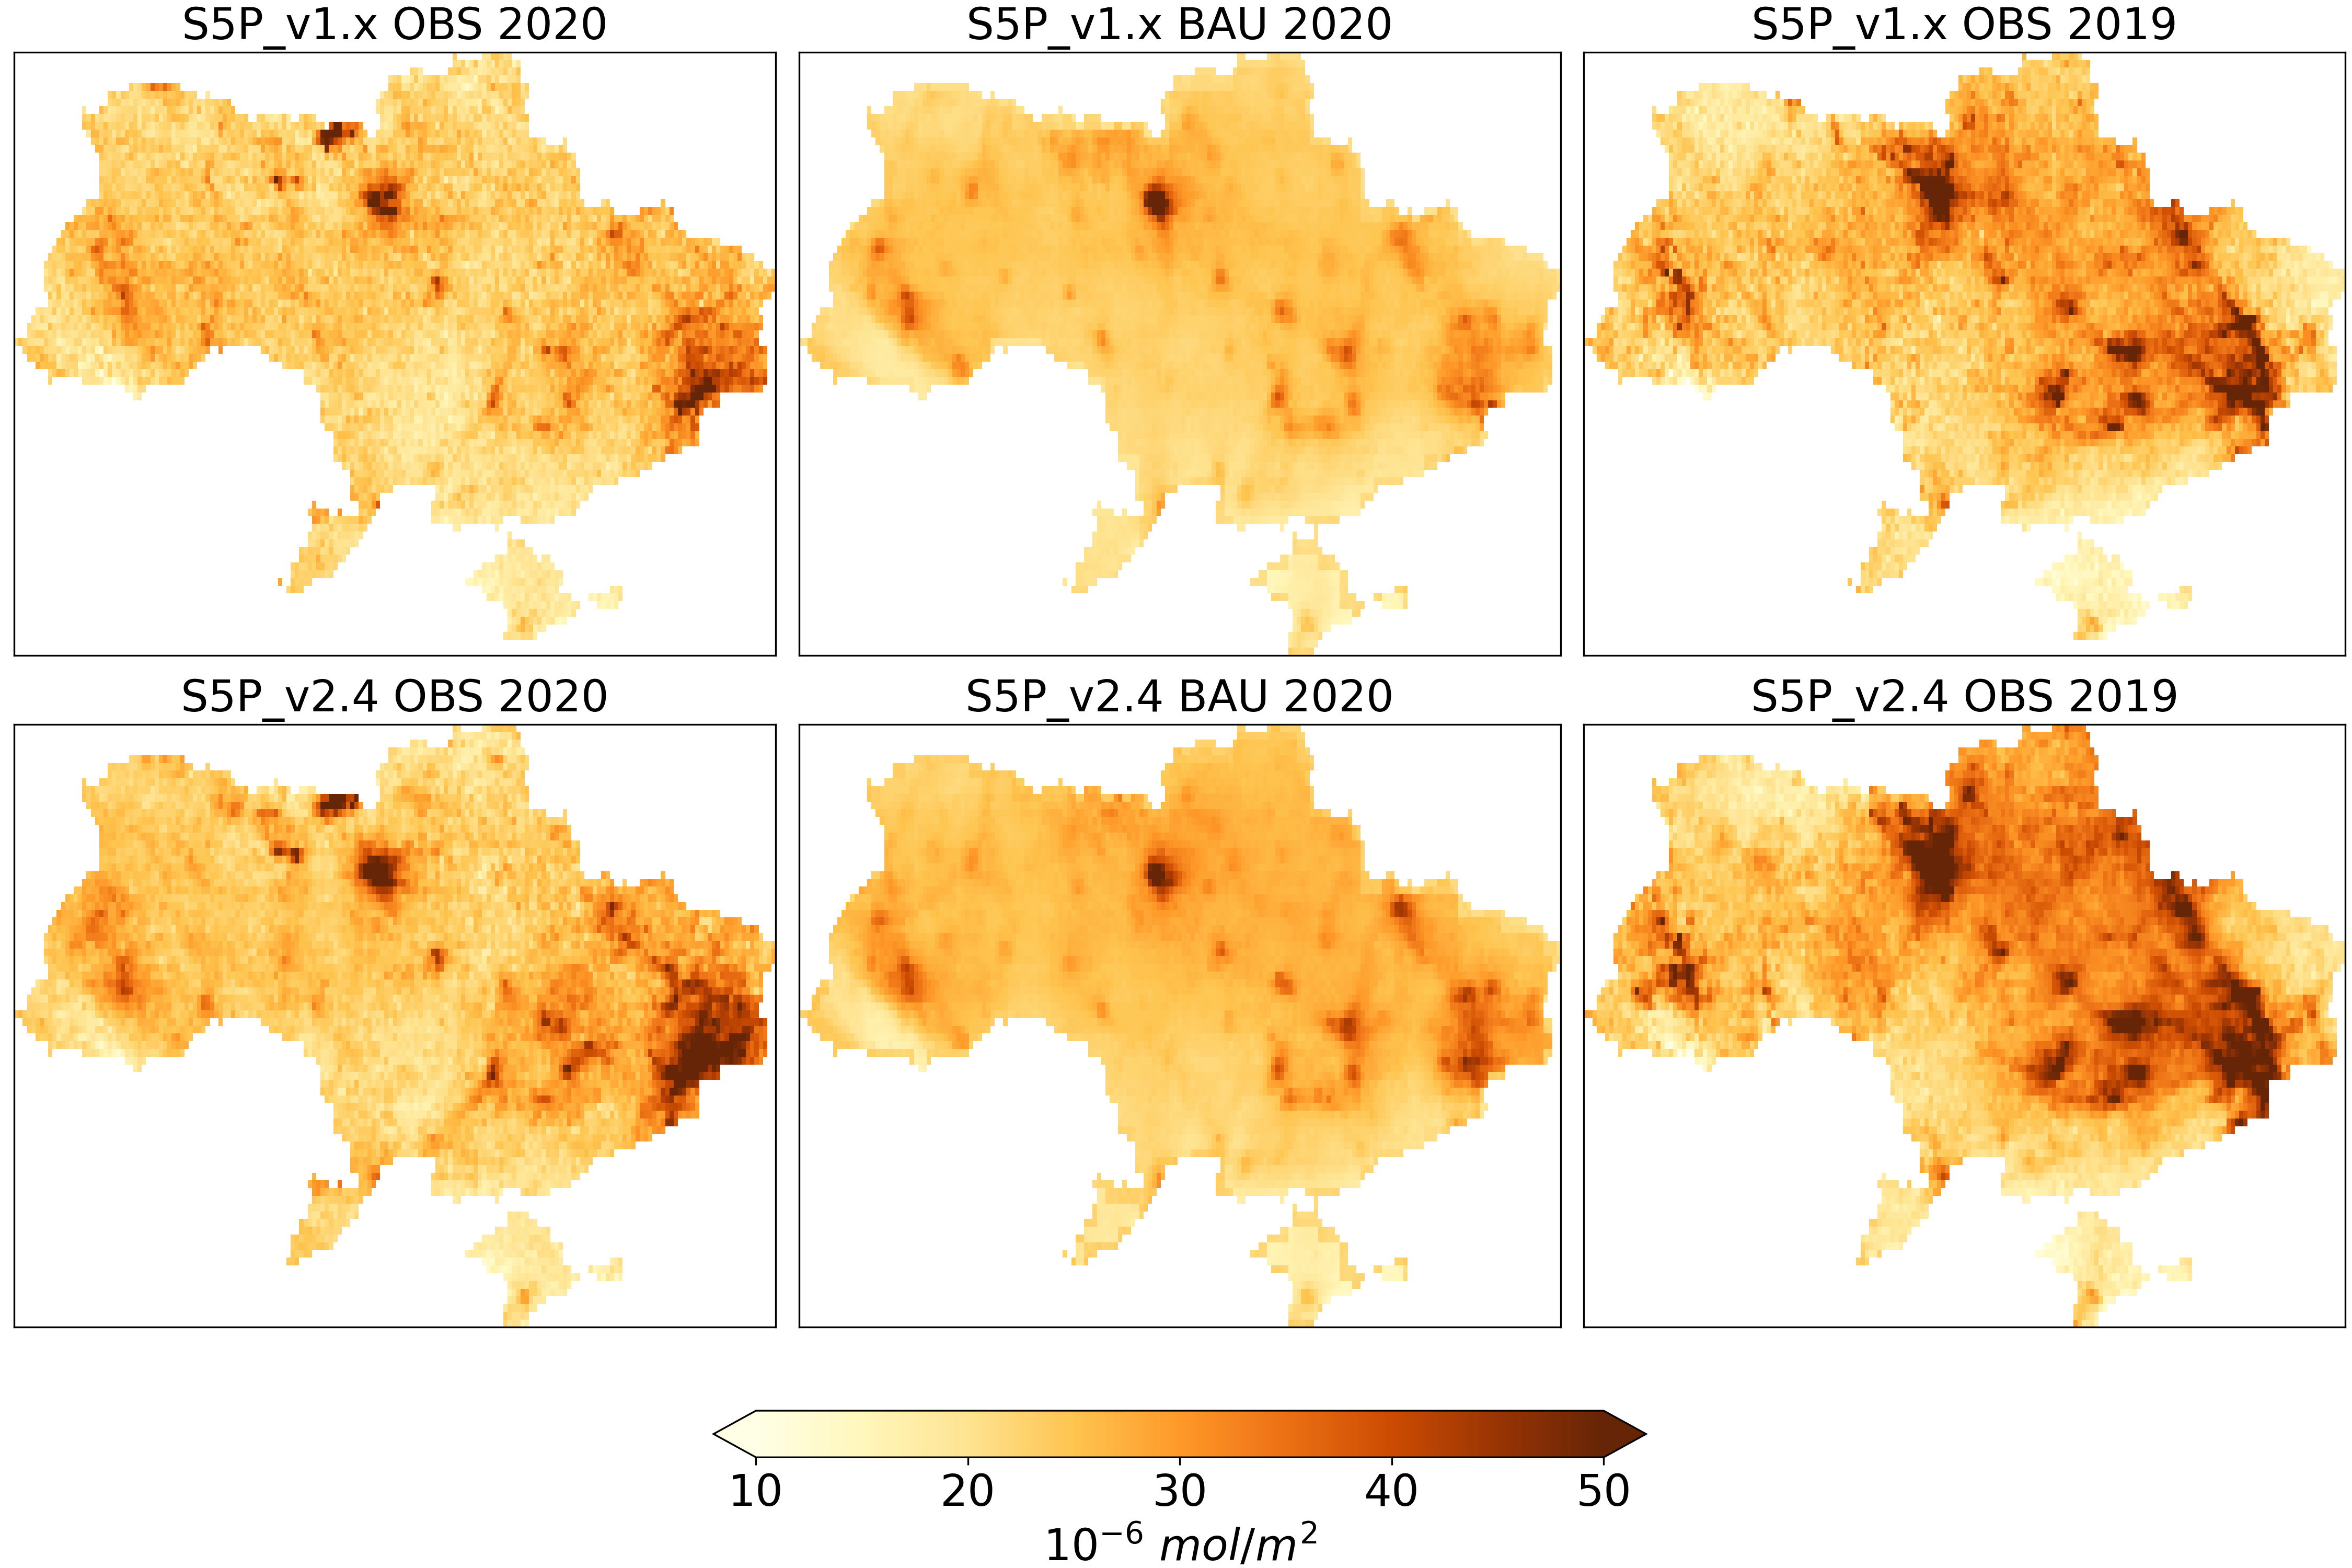
\includegraphics[width=\textwidth]{figs/chap3/figA3_a.png}
      \caption[Examples of OBS and BAU data in 2020]{The OBS, BAU data in 2020 (April 6 to May 10) with reference data in 2019}
    \end{subfigure}

    \begin{subfigure}{\textwidth}
      \centering
      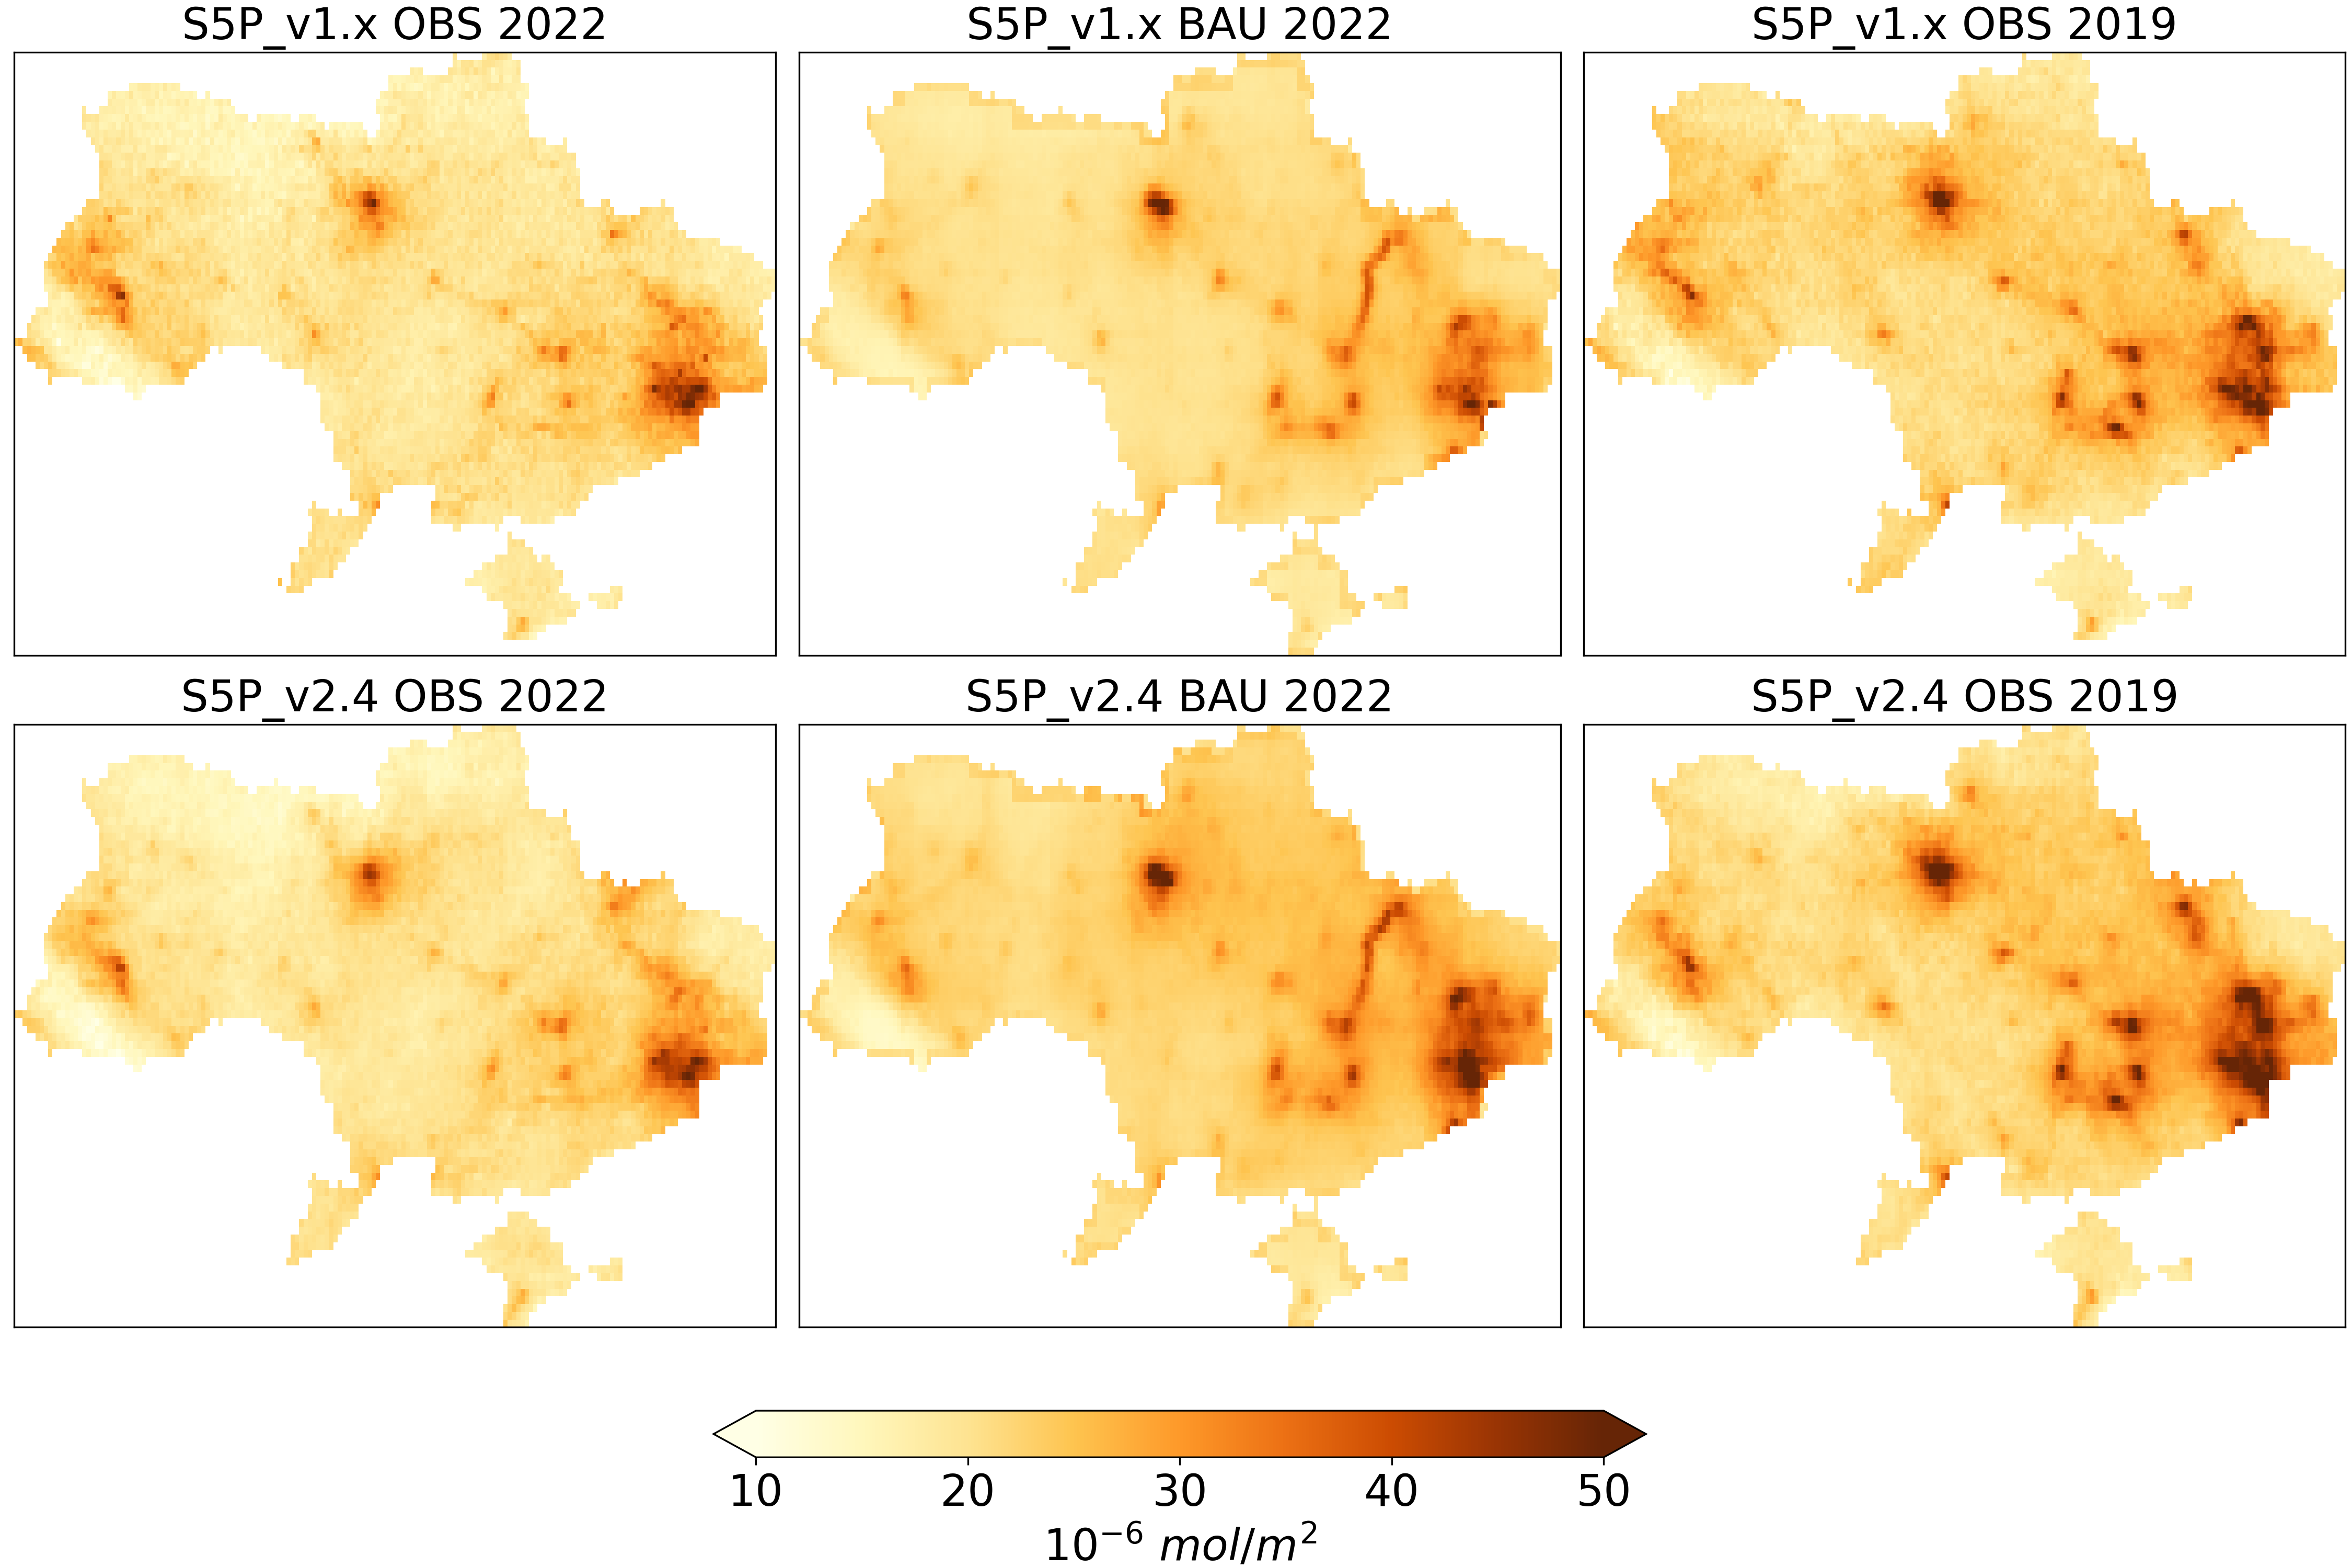
\includegraphics[width=\textwidth]{figs/chap3/figA3_b.png}
      \caption{The OBS, BAU data in 2022 (February 24 to July 31) with reference data in 2019}
    \end{subfigure}
    \caption[Examples of OBS and BAU data in 2022]{The OBS (1st column), BAU (2nd column) data from April 6 to May 10, 2020 (a)and from February 24 to July 31, 2022 (b) with the corresponding reference data in 2019 (3rdcolumn)}
    \label{fig:chap3_figa3}
\end{figure}

In order to assess the performance of the BAU simulation model, we randomly selected and used 80\% of the data for the training set and 20\% for the validation set. We used the following metrics: mean bias (MB), normalized mean bias (nMB), root mean square error (RMSE), normalized root mean square error (nRMSE) and Pearson correlation coefficient (R). As shown in the detailed results presented in Table \ref{tab:chap3_tab1}, the model achieved high R on the validation set (0.8 for ORG data, 0.86 for RPRO data), with low MB and RMSE indicating that the column NO2 levels are well represented by the input features. Based on the feature importance measure as shown in Figure \ref{fig:chap3_figa1}, we found that the most important predictors are wind speed and direction, and BLH, which is also consistent with our hypothesis about the impact of the meteorological parameters on column NO2 levels mentioned above. In Figure \ref{fig:chap3_figa2}, we present the performance of the BAU model on the validation set using trend lines and scatter plots to compare the predictions with the actual ground truth data. Furthermore, Figure \ref{fig:chap3_figa3} displays the OBS data, BAU model’s predictions during the lockdown period in 2020, and more than five months of the conflict (February 24–July 31) in 2022. This data is accompanied by the reference NO2 levels from 2019 which were utilized to train the BAU for corresponding periods. The hyperparameters used to develop the LightGBM model are listed in Table \ref{tab:chap3_taba1} for S5P data version 1.x and version 2.4. \par

\begin{table}[tbh!]
    \centering
    \caption[The hyperparameters used to develop the LightGBM model]{The hyperparameters used to develop the LightGBM model with S5P data version 1.x and version 2.4. We used FLAML library \citep{wang2021flaml} for tuning these following parameters: shrinkage rate (learning\_rate), minimal number of data in one leaf (min\_data\_in\_leaf), minimal sum hessian in one leaf (min\_sum\_hessian\_in\_leaf), number of boosting iterations (num\_iterations), max number of leaves in one tree (num\_leaves).}
    \begin{tabular}{c c c}
        \hline
            Parameter & S5P v1.x & S5P v2.4  \\ \hline
            learning\_rate & 0.30775042929674906 & 0.3858774543125185  \\
            min\_data\_in\_leaf & 11 & 5  \\
            min\_sum\_hessian\_in\_leaf & 0.001 & 0.001  \\
            num\_iterations & 907 & 3451  \\
            num\_leaves & 8604 & 4342  \\ \hline
    \end{tabular}
    \label{tab:chap3_taba1}

\end{table}

The main shortcoming of this method is the lack of qualified reference data to develop the weather normalization model under BAU conditions, as the S5P TROPOMI data has been only available since mid-2018. Only one year of training data in 2019 is considered relatively small, thus resulting in large errors in BAU simulations in winter months as during this time, limited qualified S5P observations are available and NO2 pollution levels are quite unpredictable due to the inconsistency in heating activities and NO2 intake from Poland.\par
\section{COVID-19 induced NO2 changes} \label{chap3_covid}
The purpose of this section is to examine the effect of the lockdown on changes in NO2 column levels in populous urban areas, namely the nine cities Kyiv, Kharkiv, Odessa, Dnipro, Donetsk, Zaporizhzhia, Lviv, Kryvyi Rih, and Mykolaiv (listed in declining order of population). To begin, we analyse the meteorological patterns during the pre-lockdown and lockdown periods and discuss how these might influence the NO2 levels, apart from the impacts of the lockdown measures. Next, we utilize two methods to estimate changes in NO2 levels. The first method, known as the year-to-year approach suggested by \citep{barre2021estimating}, involves calculating the median value of the actual S5P observation data in 2020 and subtracting the observation data from 2019. The second method, OBS-BAU, utilizes the median value of the actual observation data (OBS) in 2020 and subtracts the simulated NO2 levels that represent the BAU scenario, which are predicted by the S5P tropospheric NO2 column levels without any lockdown measures. The BAU simulations are based on the representation of meteorological, spatial, and temporal parameters. \par
\subsection{Lockdown and pre-lockdown meteorological patterns}
Figure \ref{fig:chap3_fig3a} and \ref{fig:chap3_fig3b} display the probability density functions of the BLH, and Figure \ref{fig:chap3_fig4a} and \ref{fig:chap3_fig4b} display wind speed and direction during the pre-lockdown and lockdown periods of 2019 and 2020 based on data from the nine selected cities. In 2020, the BLH exhibited a similar distribution to that of 2019 during the pre-lockdown period, but with lower values. This decrease in BLH would have resulted in an increase in NO2 levels in 2020 compared to 2019, as the reduced BLH restricts the dispersion of NO2 emissions, leading to an increase in NO2 concentration levels (see Figure \ref{fig:chap3_fig3a}). \par

\begin{figure}[tbh!]
    \centering
    \begin{subfigure}{.5\textwidth}
      \centering
      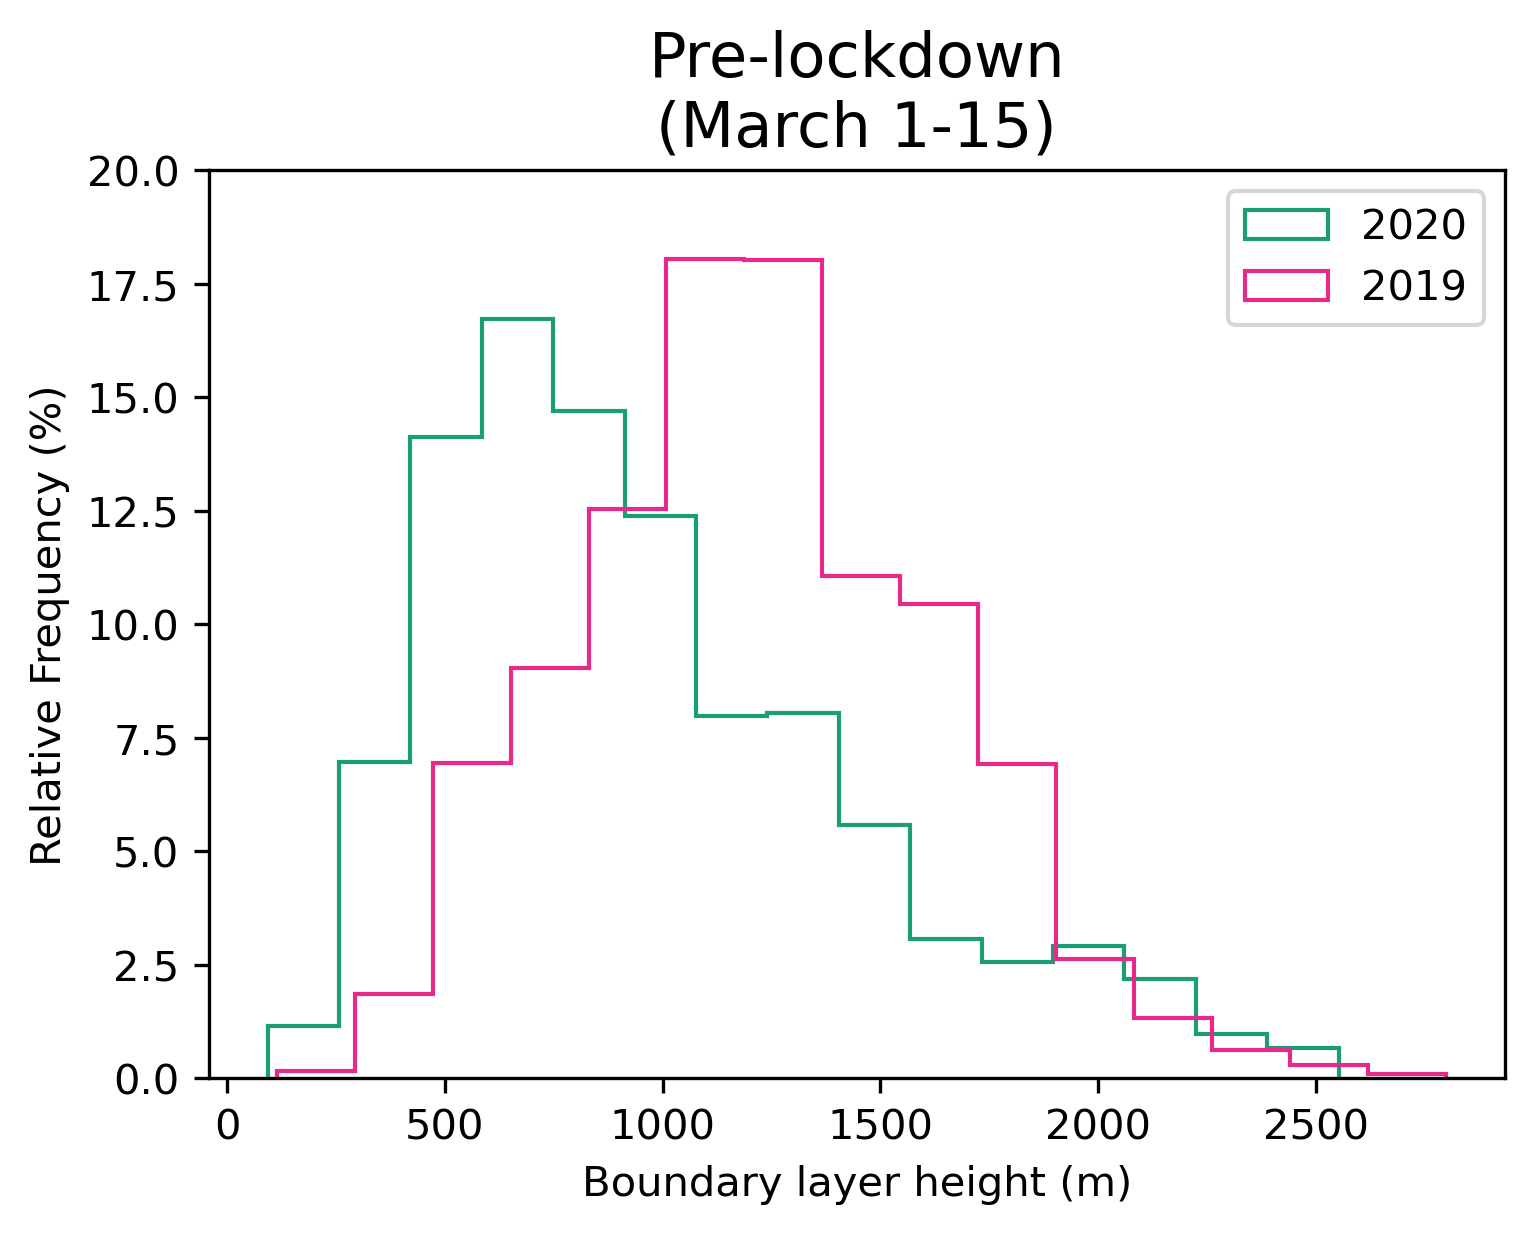
\includegraphics[width=\textwidth]{figs/chap3/fig3_a.png}
      \caption{}
      \label{fig:chap3_fig3a}
    \end{subfigure}%
    \begin{subfigure}{.5\textwidth}
      \centering
      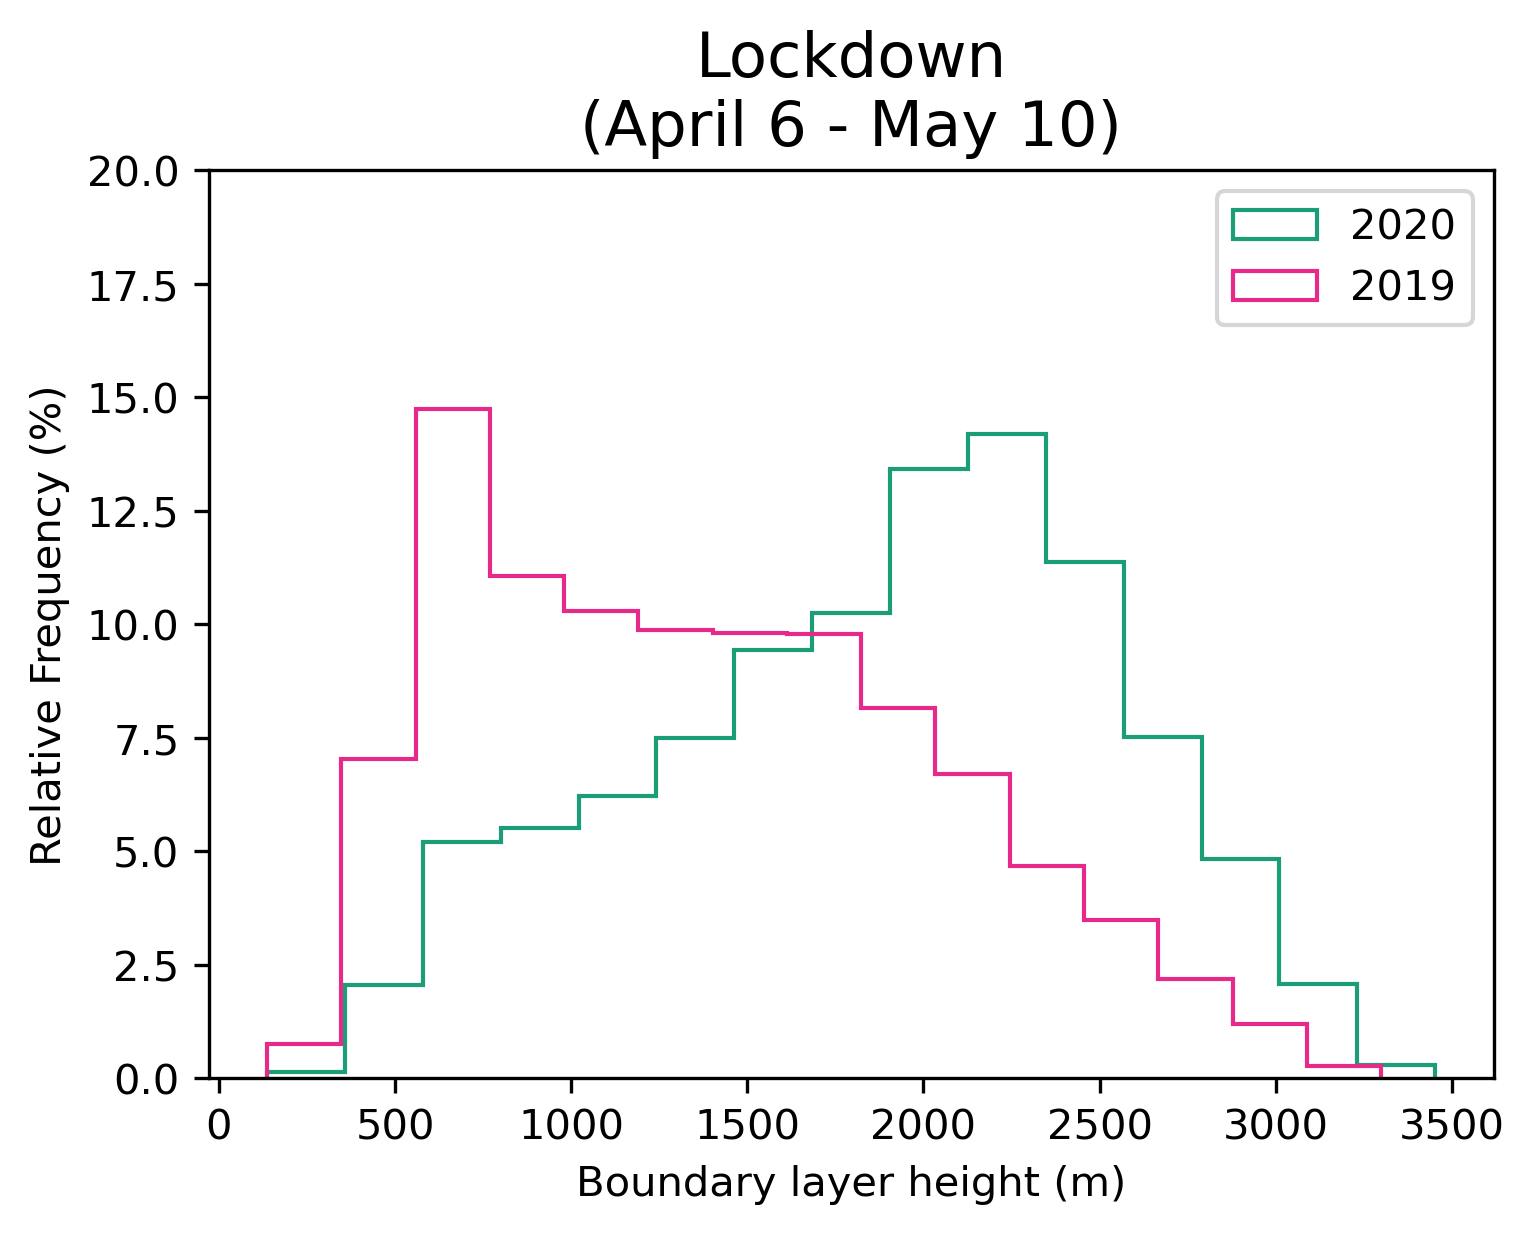
\includegraphics[width=\textwidth]{figs/chap3/fig3_b.png}
      \caption{}
      \label{fig:chap3_fig3b}
    \end{subfigure}
    \begin{subfigure}{.5\textwidth}
        \centering
        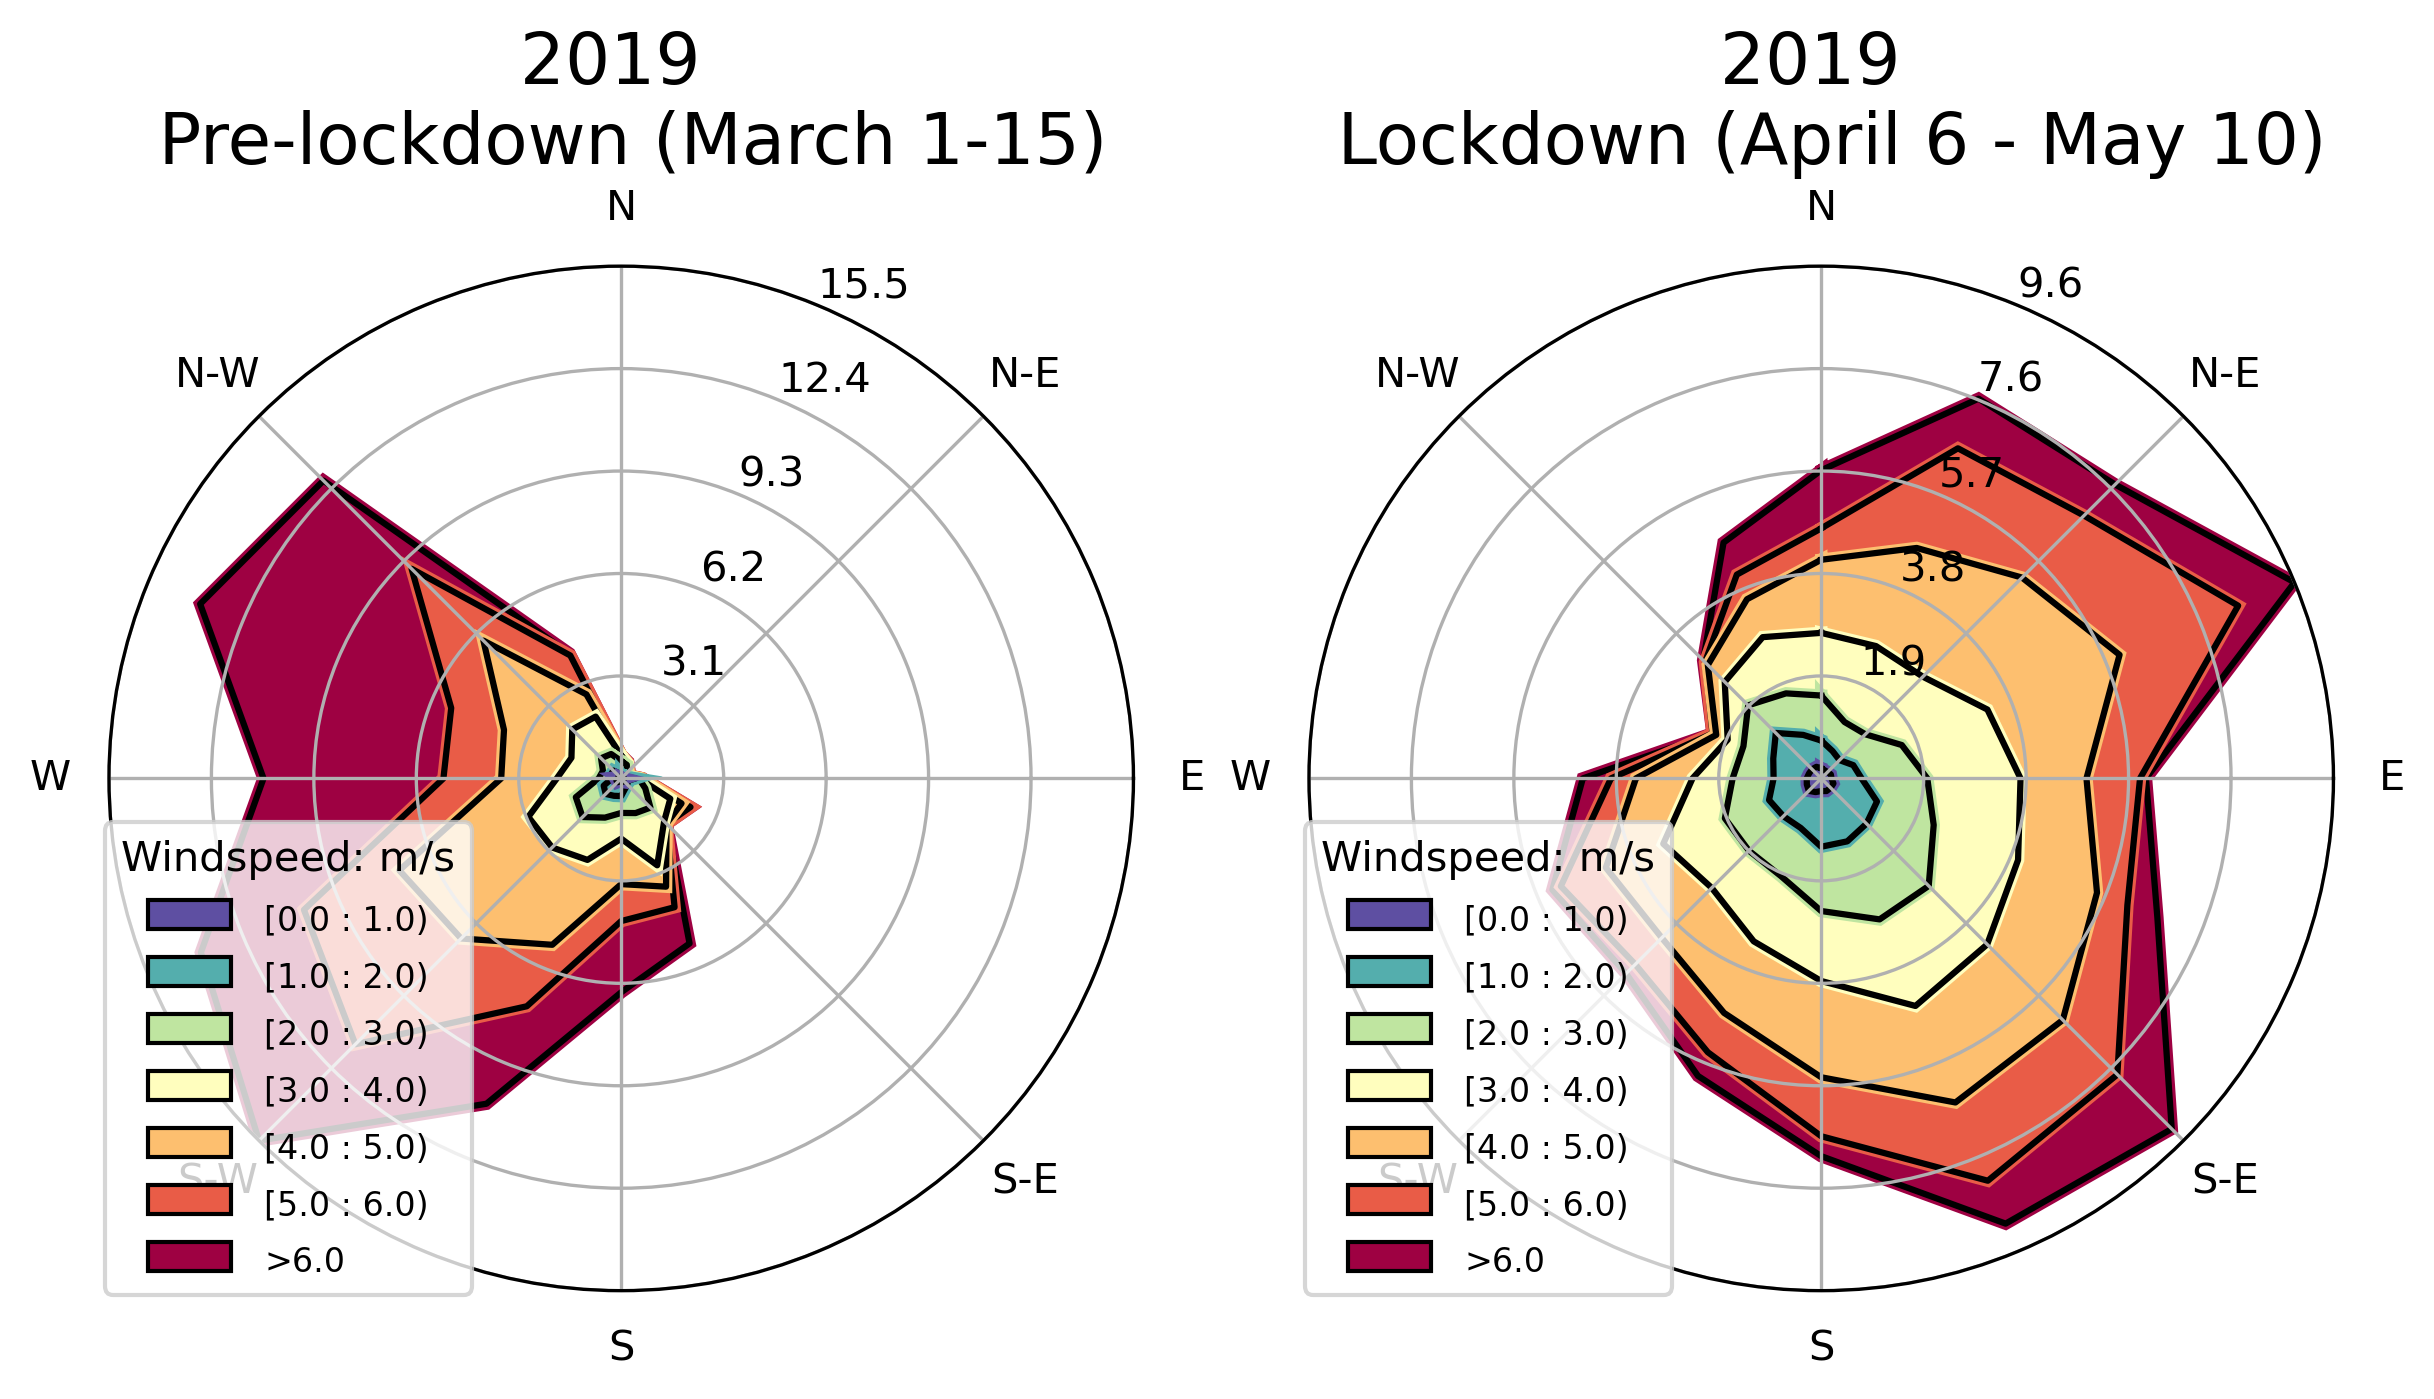
\includegraphics[width=\textwidth]{figs/chap3/fig4_a_2019.png}
        \caption{}
        \label{fig:chap3_fig4a}
    \end{subfigure}%
    \begin{subfigure}{.5\textwidth}
        \centering
        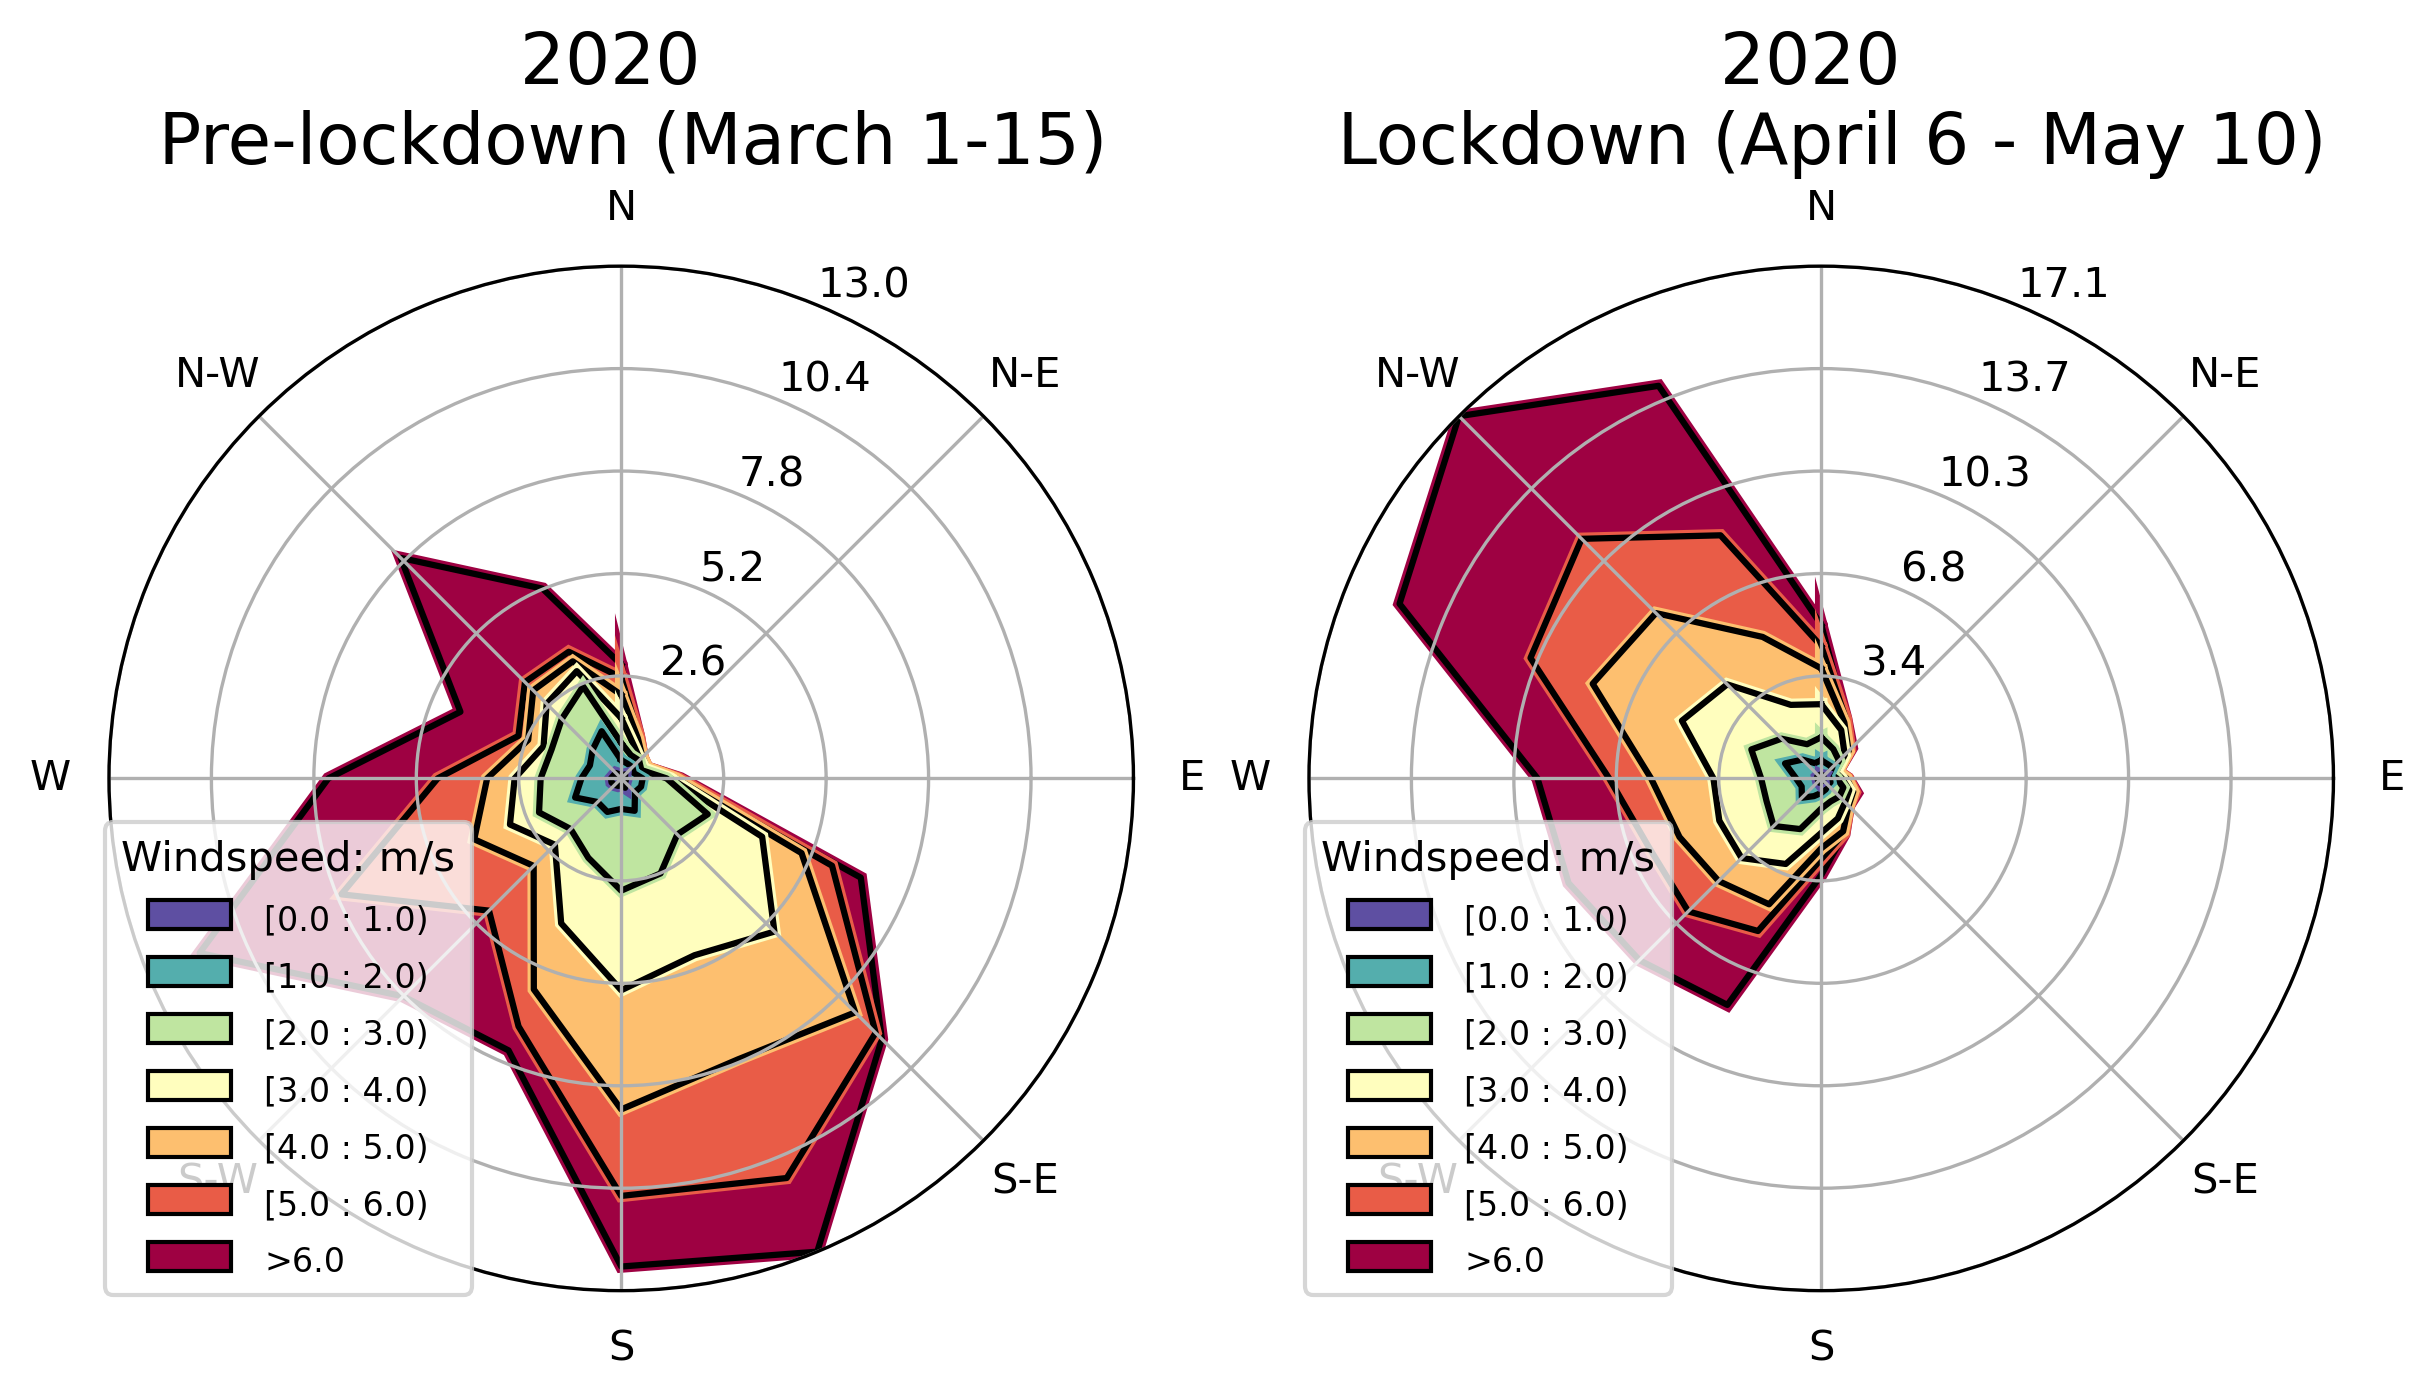
\includegraphics[width=\textwidth]{figs/chap3/fig4_b_2020.png}
        \caption{}
        \label{fig:chap3_fig4b}
    \end{subfigure}
    \caption[Meteorological variations during pre-lockdown and lockdown]{Probability density functions of BLH during (a) the pre-lockdown (March 1–15) and (b) the lockdown period (April 6–May 10) between 2019 and 2020 based on data from the nine most populous cities of Ukraine. Wind rose plots for wind speed and direction for pre-lockdown (March 1–15) and lockdown (April 6–May 10) periods in (c) 2019 and (d) 2020 based on data from the nine most populous cities of Ukraine}
    \label{fig:chap3_fig34}
\end{figure}

Conversely, during the lockdown period (see Figure \ref{fig:chap3_fig3b}), we observed higher values of BLH in 2020 compared to 2019. This increase in BLH could have contributed to the dispersion of NO2 concentration, resulting in a reduction of NO2 levels during the lockdown in 2020. This phenomenon, in addition to the effects of the lockdown restrictions, may have also contributed to minimizing the NO2 levels over major cities in Ukraine. Therefore, it is essential to consider the impacts of meteorological variables on NO2 level variability analysis.\par


\subsection{NO2 changes in populous Ukrainian cities}
In Figures (\ref{fig:chap3_fig5a}, \ref{fig:chap3_fig5b}), and Table \ref{tab:chap3_tab2}, we present the result of the year-to-year approach. We assumed that there would be a minimal change in NO2 pollution levels during the pre-lockdown period, but a significant reduction during the lockdown when comparing the same time frame in 2019 and 2020 due to the implemented lockdown measures and social distancing practices. In Figure \ref{fig:chap3_fig5}, two different methods, namely the OBS-BAU and year-to-year approaches, were used for the analysis. The circle size in the figures corresponds to the population of each city. For each sub-figure (a) and (b), the first row (a1, a2, b1, b2) contains two plots showing the results based on the ORG data (S5P v1.x), while the second row (a3, a4, b3, b4) includes two plots presenting the results based on the RPRO data (S5P v2.4). The left column plots (a1, a3, b1, b3) of Figures (\ref{fig:chap3_fig5a}, \ref{fig:chap3_fig5b}) display the year-to-year estimates, while the right column plots (a2, a4, b2, b4) display the OBS-BAU estimates. Figure \ref{fig:chap3_fig5a} illustrates that the prevailing trend in the nine selected cities during the pre-lockdown period showed an increase, with an average of 5.2\% (ORG data) and 13.9\% (RPRO data) in NO2 levels, while during the lockdown period (Figure \ref{fig:chap3_fig5b}), a general reduction was observed in most cities with an average of 15.6\% (ORG data) and 11.1\% (RPRO data). This confirms that the lockdown measures reduced the NO2 column concentrations in major urban areas of Ukraine, as we anticipated. It is worth noting that the year-to-year approach using the original satellite observations has been widely used in many studies and online resources. However, as mentioned in \citep{barre2021estimating,grange2021covid}, it is heavily influenced by meteorological variables such as wind speed and direction, and BLH \citep{wallace2009effect}.\par

\begin{figure}[p]
    \centering
    \begin{subfigure}{\textwidth}
      \centering
      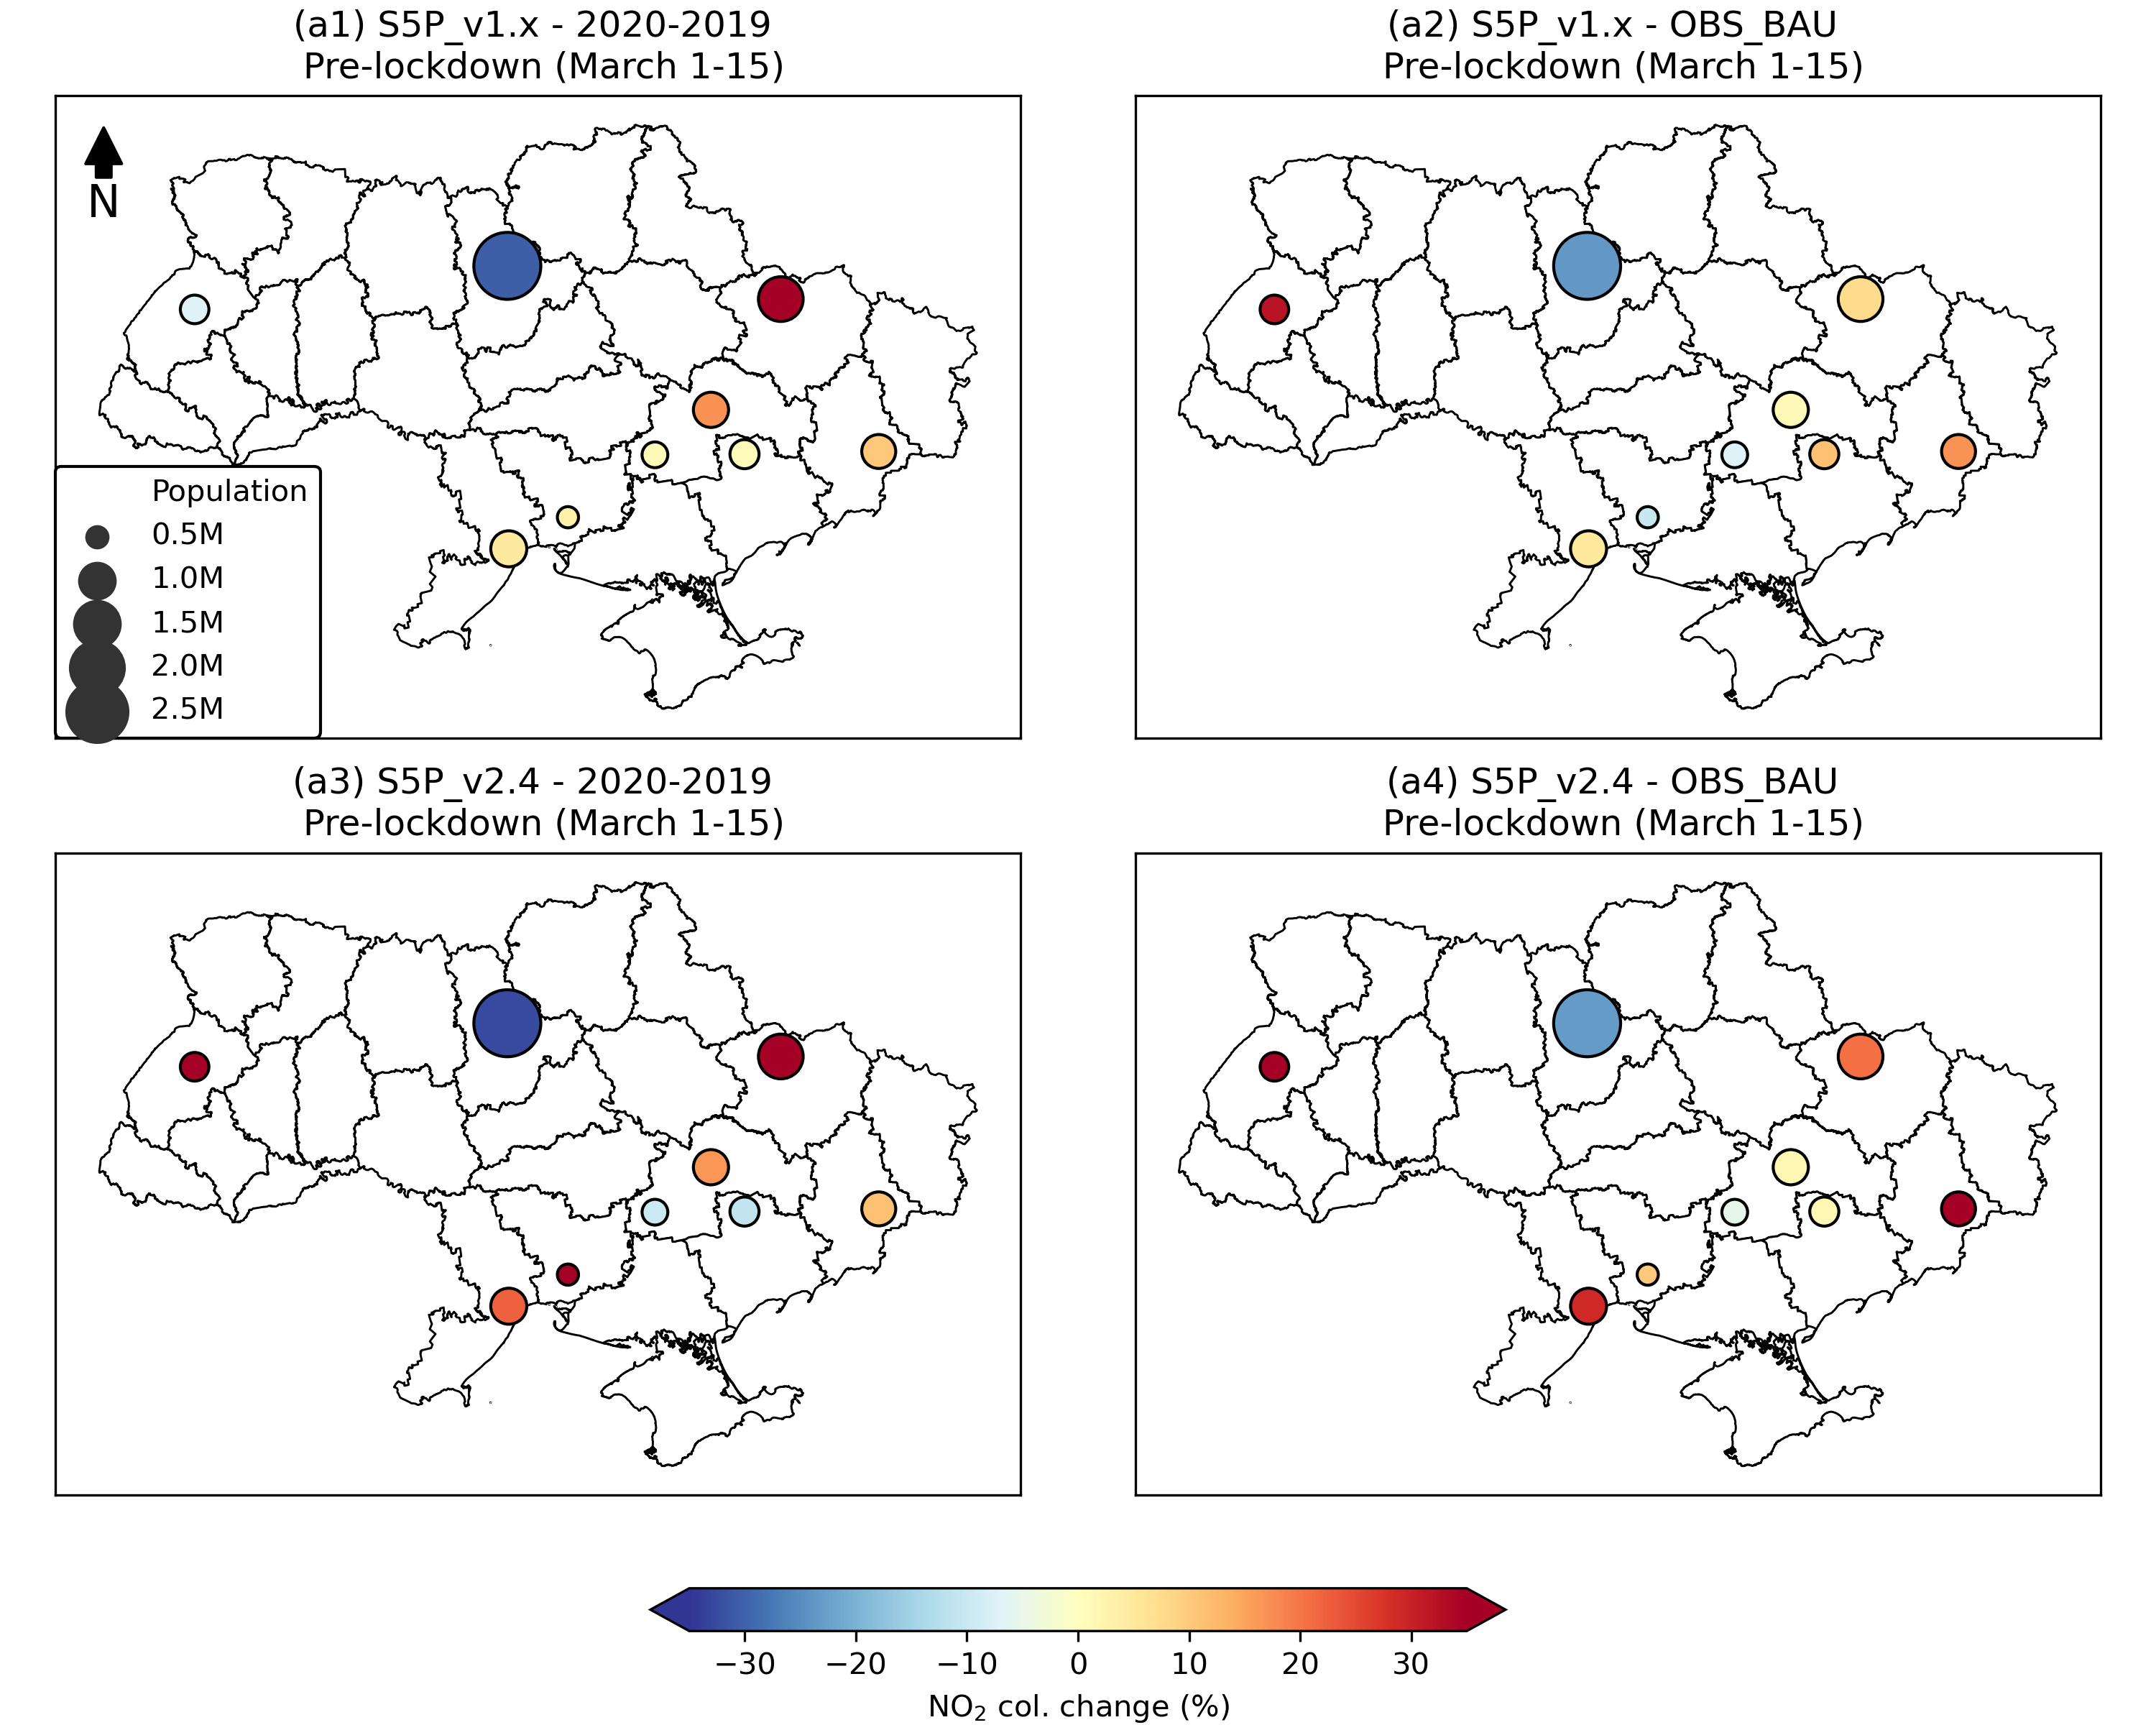
\includegraphics[width=.8\textwidth]{figs/chap3/fig5_a.png}
      \caption{Pre-lockdown period}
      \label{fig:chap3_fig5a}
    \end{subfigure}

    \begin{subfigure}{\textwidth}
      \centering
      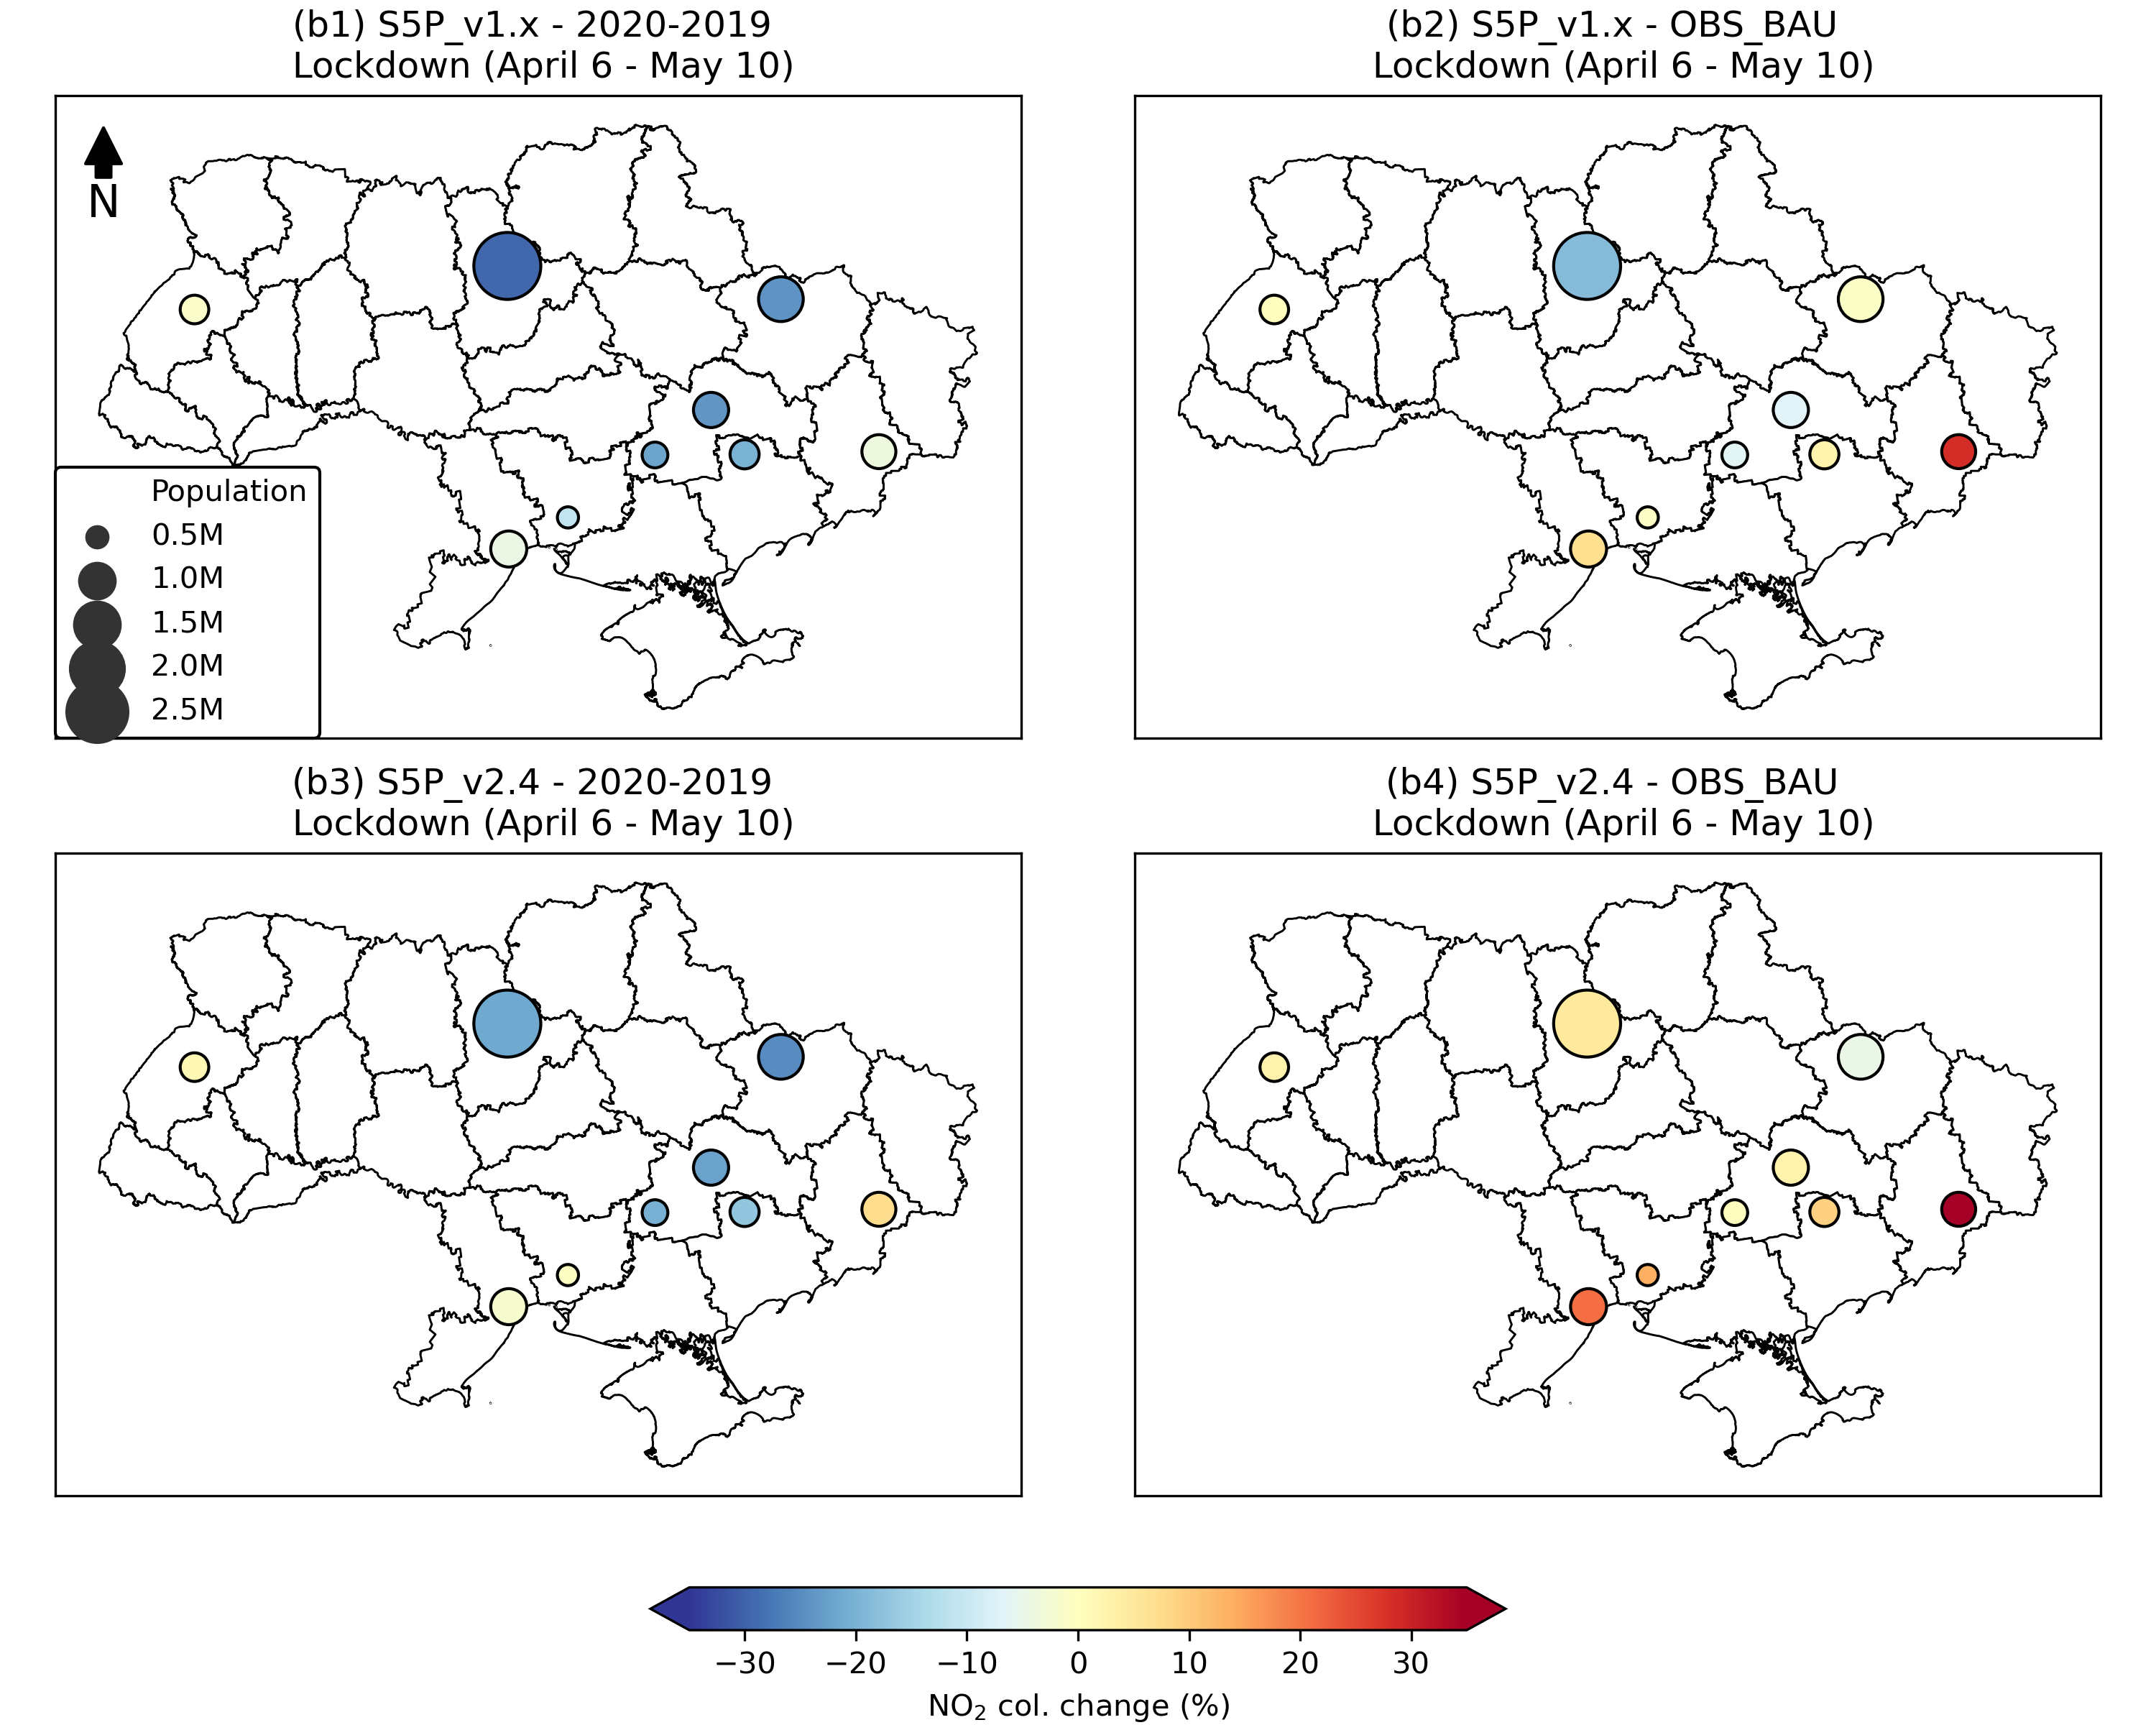
\includegraphics[width=.8\textwidth]{figs/chap3/fig5_b.png}
      \caption{Lockdown period}
      \label{fig:chap3_fig5b}
    \end{subfigure}
    \caption[S5P NO2 level changes for most populous cities]{Estimates of S5P NO2 column changes for the nine most populous cities in Ukraine during the (a) pre-lockdown and (b) lockdown periods.}
    \label{fig:chap3_fig5}
\end{figure}

\begin{table}[!ht]
    \centering
    \caption[S5P NO2 level changes estimates for most populous cities]{The OBS-BAU and year-to-year (2020–2019) estimates (in percentage) during pre-lockdown and lockdown periods in the nine most populous cities in Ukraine. The values are represented as mean, while standard deviation is not presented here due to lack of space.}
    \begin{adjustbox}{width=\textwidth}
      \begin{tabular}{l c c c c c c c c}
      \hline
          \multirow{3}{*}{City} & \multicolumn{4}{c}{Pre-lockdown (March 1 \textminus 15)} & \multicolumn{4}{c}{Lockdown (April 6 \textminus May 10)} \\ \cline{2-9}
              ~& \multicolumn{2}{c}{OBS-BAU} & \multicolumn{2}{c}{2020\textminus2019} & \multicolumn{2}{c}{OBS-BAU} & \multicolumn{2}{c}{2020\textminus2019} \\ \cline{2-9}
              ~& ORG & RPRO & ORG & RPRO & ORG & RPRO & ORG & RPRO \\ \hline
          Kyiv & \textminus23.7 & \textminus23.1 & \textminus30.6 & \textminus32.8 & \textminus18.8 & 4.9 & \textminus29.4 & \textminus21.4  \\
          Kharkiv & 7.6 & 20.8 & 47.9 & 49.1 & \textminus0.9 & \textminus4.9 & \textminus24.1 & \textminus24.9  \\
          Odessa & 5.1 & 29.0 & 4.8 & 22.4 & 6.9 & 21.0 & \textminus4.4 & \textminus1.9  \\
          Dnipro & 1.3 & 1.5 & 17.0 & 16.7 & \textminus6.6 & 2.8 & \textminus23.9 & \textminus22.3  \\
          Donetsk & 16.8 & 41.9 & 10.3 & 11.2 & 28.2 & 42.0 & \textminus4.0 & 7.2  \\
          Zaporizhzhia & 11.5 & 1.9 & 0.6 & \textminus11.1 & 2.5 & 9.1 & \textminus20.1 & \textminus17.2  \\
          Lviv & 32.2 & 35.7 & \textminus7.3 & 37.7 & 0.0 & 3.0 & \textminus1.2 & 1.4  \\
          Kryvyi Rih & \textminus7.3 & \textminus5.3 & 1.2 & \textminus9.8 & \textminus6.4 & 0.1 & \textminus21.9 & \textminus20.5  \\
          Mykolaiv & \textminus10.2 & 10.1 & 3.3 & 41.5 & \textminus0.6 & 13.8 & \textminus11.1 & \textminus0.4  \\
          Mean & 3.7 & 12.5 & 5.2 & 13.9 & 0.5 & 10.2 & \textminus15.6 & \textminus11.1 \\ \hline
      \end{tabular}
    \end{adjustbox}
    \label{tab:chap3_tab2}
\end{table}

In order to quantify the true improvement in air quality with respect to column NO2 levels due to the lockdown restrictions, we calculated the difference between the actual observation data and the simulated data under BAU conditions with the meteorological effects decoupled. Like the year-to-year approach, we anticipate a slight variation between the OBS NO2 levels and the BAU NO2 levels during the pre-lockdown period. Furthermore, we expect to observe an overall reduction in the OBS data compared to the BAU data, or at least, a lesser increase during the lockdown when compared to the pre-lockdown levels, due to the impact of the lockdown measures. Figure \ref{fig:chap3_fig5}((a2, a4) and (b2, b4)) shows the OBS-BAU estimates for pre-lockdown and lockdown in 2020. During the pre-lockdown (Figure \ref{fig:chap3_fig5}(a2, a4)), we observed an average increase of 3.7\% (ORG data) and 12.5\% (RPRO data), which is smaller than the year-to-year estimate. However, during the lockdown period (Figure \ref{fig:chap3_fig5}(b2, b4)) a smaller increase trend was observed, with an average of 0.5\% (ORG data) and 10.2\% (RPRO data). This indicates that while the OBS NO2 levels in 2020 were higher than those predicted under the BAU scenario during the lockdown period, the measures implemented during the lockdown effectively curbed the increase in NO2 column concentrations in major urban areas of Ukraine when compared to the pre-lockdown levels, aligning with our initial expectations. By using the OBS-BAU estimate based on the ORG data, the most significant reduction was observed in Kyiv (18.8\%), with Dnipro and Kryvyi Rih experiencing smaller reductions of 6.6\% and 6.4\%, respectively. However, when using RPRO data, a reduction was only seen in Kharkiv (4.9\%).\par

In comparison with the year-to-year approach with respect to the pre-lockdown (see Table \ref{tab:chap3_tab2}), the OBS-BAU estimates (3.7\% for ORG data, 12.5\% for RPRO data) show a smaller change than in year-to-year estimates (5.2\% for ORG data, 13.9\% for RPRO data). We consider the OBS-BAU estimate to be more reasonable as mentioned above, and the lower values in BLH in 2020 could result in higher year-to-year estimates during the pre-lockdown period between 2020 and 2019. Therefore, we anticipate a lower estimate, which is a smaller increase, after the weather effects are decoupled. Similar findings are seen during the lockdown for OBS-BAU and year-to-year estimates. The contribution from the lower BLH in 2019 could overestimate the reduction of NO2 concentrations by 15.6\% (ORG data) and 11.1\% (RPRO data) in the year-to-year lockdown estimates. By normalizing the weather effects, a lower reduction in the increase is anticipated and estimated from the OBS-BAU approach (0.5\% for ORG data, 10.2\% for RPRO data). Additionally, the year-to-year approaches mostly present a larger standard deviation than the OBS-BAU approach, which could be attributed to local biases caused by meteorological variabilities \citep{barre2021estimating}. Using weather-normalization techniques, we observed that much of the reduction in NO2 levels between 2020 and 2019 can be attributed to weather variability. This suggests that stricter measures may need to be considered in the future to achieve significant NO2 reductions in densely populated areas of Ukraine.\par

\section{NO2 changes induced by the armed conflict} \label{chap3_war}
In the previous section, we discussed the influence of meteorological factors on the concentration of NO2 and how using OBS-BAU estimates can mitigate overestimation or underestimation in the year-to-year approach. In this section, we shift our focus solely to the OBS-BAU estimates to explore the impacts of the armed conflict on NO2 column concentration. The year-to-year estimates are displayed together for the purpose of comparison.\par

During the lockdown, one might reasonably assume that pollution levels were likely to decrease as the result of an anticipated reduction in socio-economic activities in major urban areas. However, trends in NO2 levels during the conflict are likely to be unpredictable in the chaos of armed conflict actions and regionally attributed to various type of emissions at multiple locations, especially at the beginning of the conflict. On one hand, the NO2 levels should be expected to decline as anthropogenic emissions would be expected to decline due to minimized activities in transportation, industry and other socio-economic activities. On the other hand, surges in conflict activities – such as attacks with missiles, artillery shelling, bomb and mine explosions, etc., as well as the constant usage of military vehicles and the transportation of civilian populations from conflict zones in such a short time – could result in a rise in air pollution levels. Therefore, we extend our study beyond the most populous cities and include other territories in Ukraine affected by the conflict. To accomplish this, we begin by locating the conflict hotspots where military actions and battles took place, and then analyse the changes in NO2 concentrations in the hotspots, which are highly contested zones. We estimated the changes in pollution levels from individual conflict points, and the results are presented in Section 5.1. In Section 5.2, we analyse the impacts of the conflict on NO2 levels in other affected regions, such as major cities with populations exceeding 0.5 million, and the areas surrounding CPPs.\par
\subsection{S5P NO2 level changes in conflict hotspots}
\subsubsection*{Satellite-captured fire spots and statistics in conflict hotspots}
To understand the distribution of conflict hotspots, we utilized both the satellite-capture fire data from the NASA FIRMS portal, and in particular, the locations of battles provided by ACLED \citep{raleigh2010introducing}. First, we inspect the fire data from the VIIRS fire product for two consecutive years (2021 and 2022), searching for patterns representing the appearance of conflict hotspots. Then, we visually compare the pattern of fire spots captured by satellite with the reported battle locations.\par

\begin{figure}[tbh!]
    \centering
    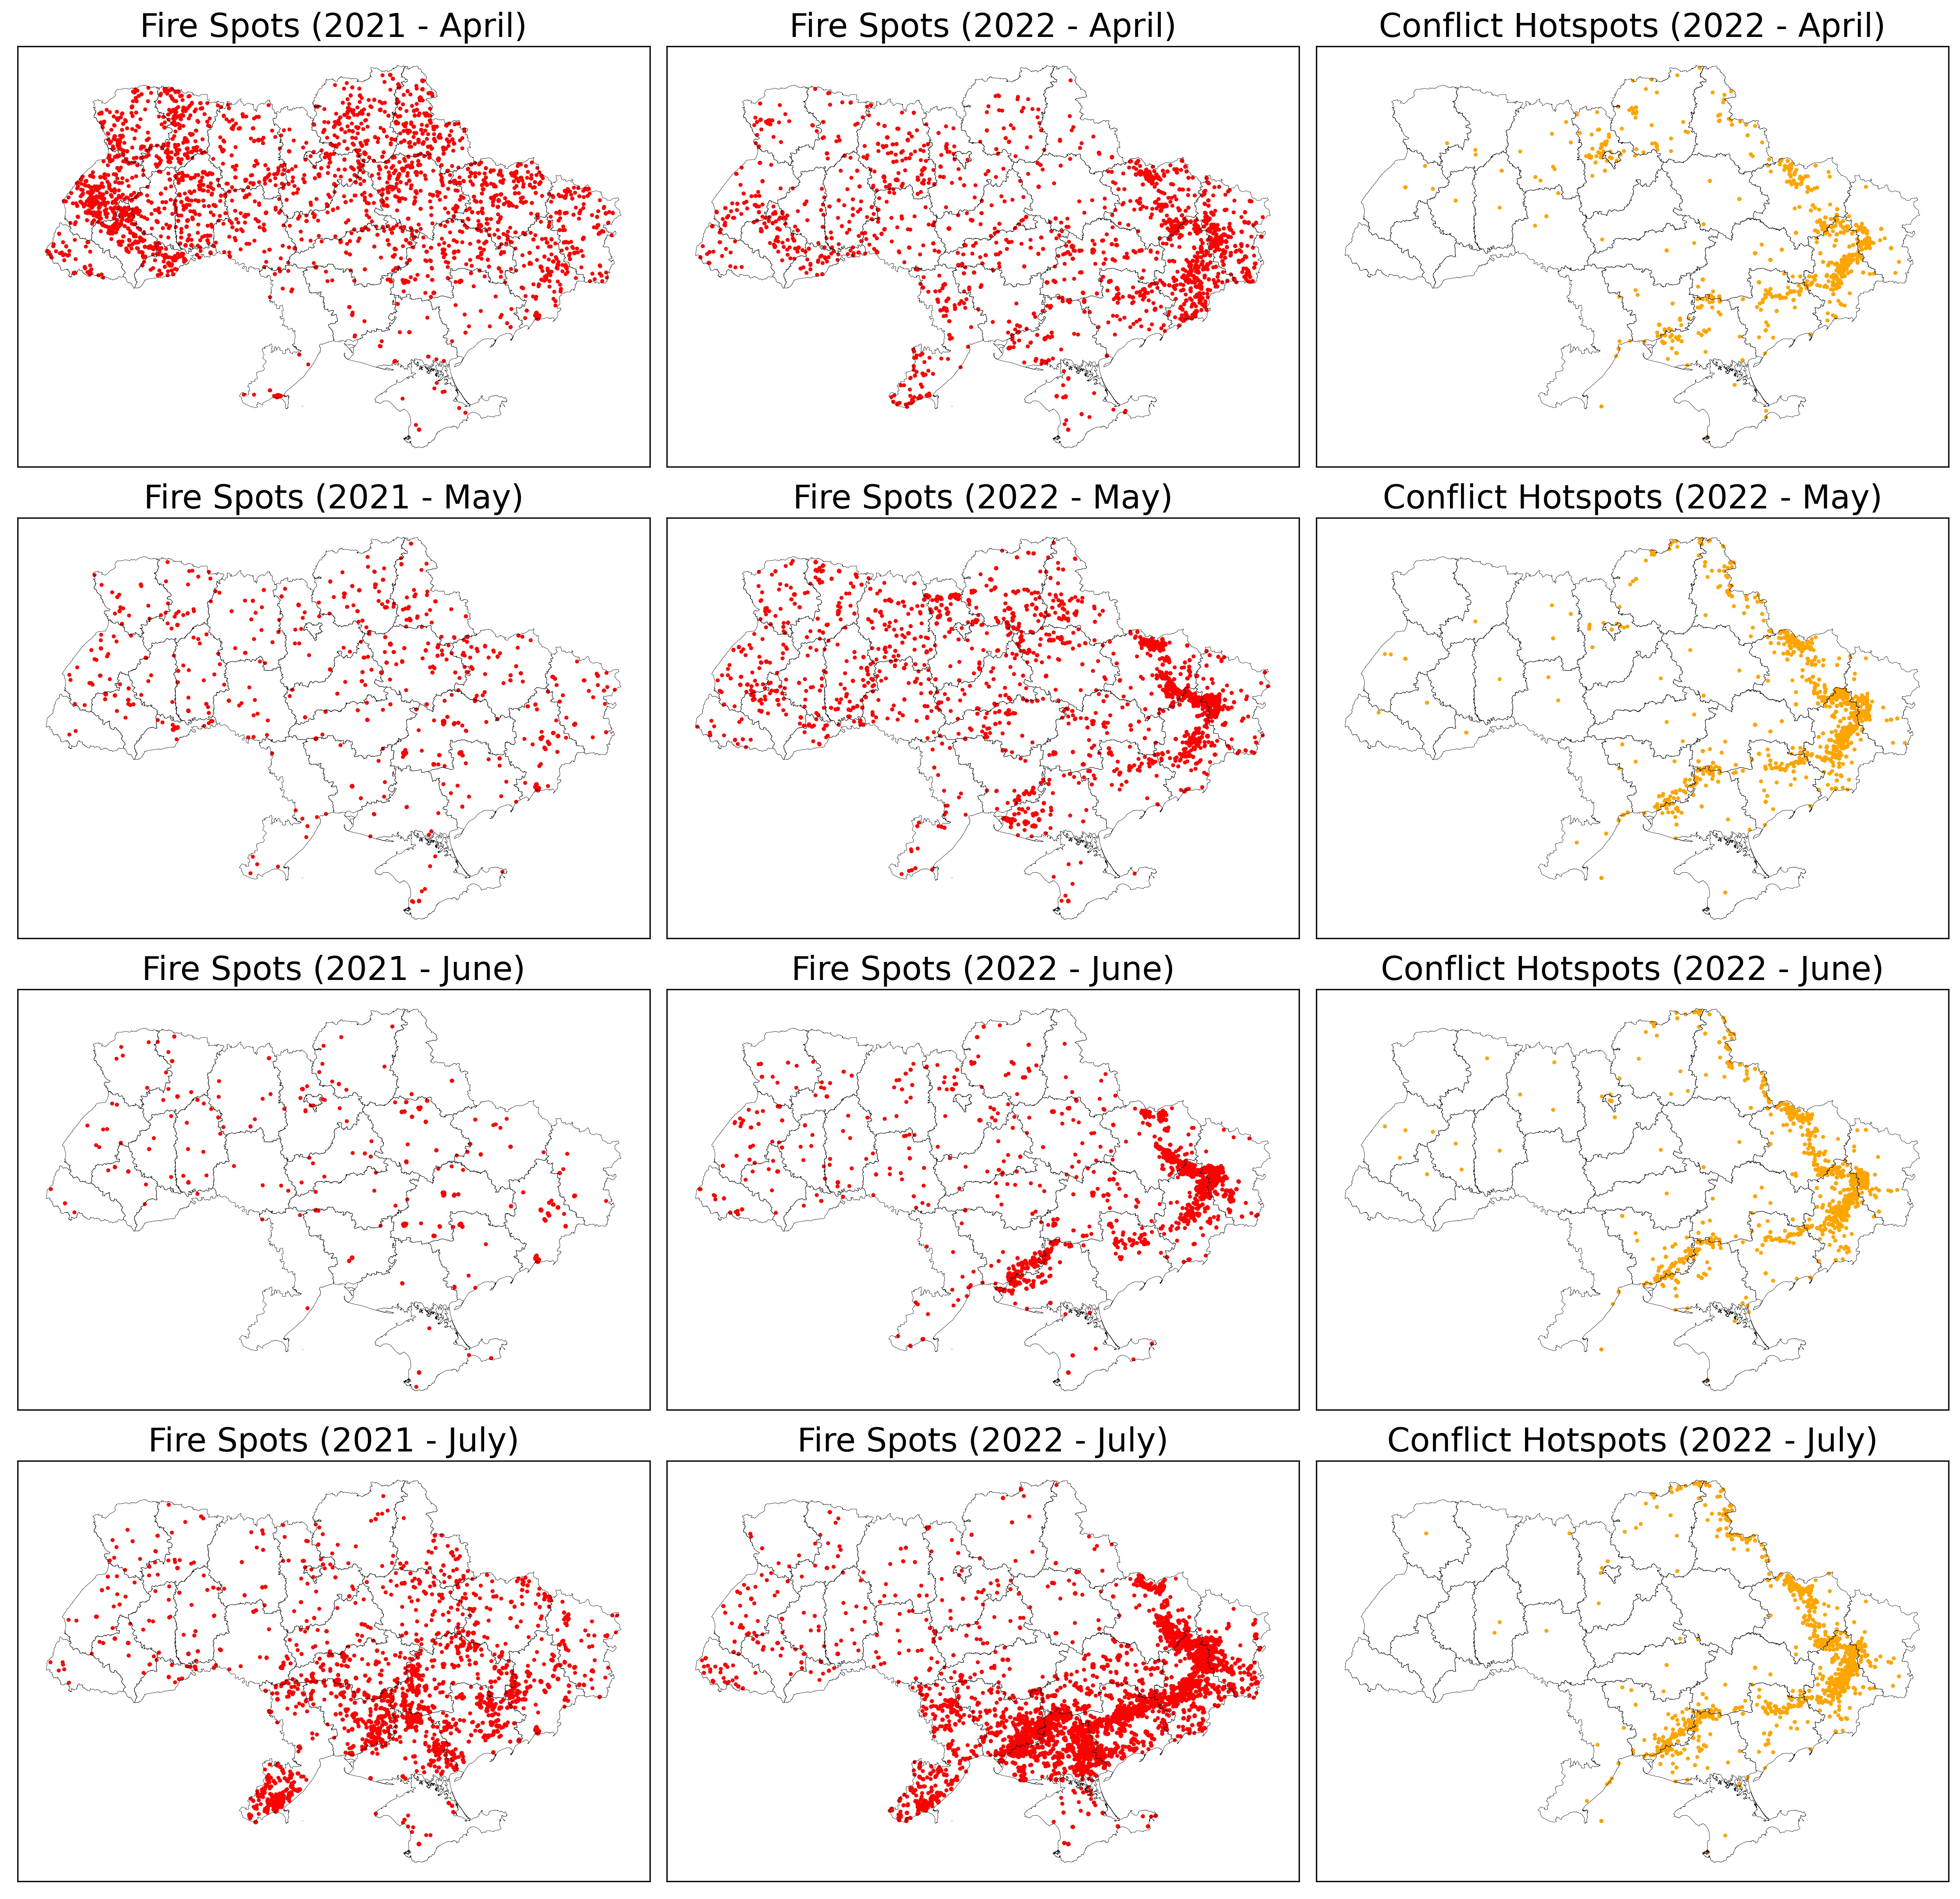
\includegraphics[width=\textwidth]{figs/chap3/fig6.png}
    \caption[Analyzed conflict hotspots using satellite and ACLED data]{Satellite-captured fire spots for 2021 (1st column), 2022 (2nd column) and conflict hotspots (3rd column) in April, May, June and July. The patterns of conflict hotspots are clearly recognizable in the satellite-capture fire product from NASA FIRMS}
    \label{fig:chap3_fig6}
\end{figure}

Figure \ref{fig:chap3_fig6} displays the satellite-captured fire spots for 2021 (1st column), 2022 (2nd column) and locations of conflict hotspots (3rd column). We only show the similar patterns captured from the monthly NASA FIRMS product and the reported conflict hotspot locations from Ukraine Crisis Hub, to avoid the overwhelming plots of 12 months. We observe that from February 24 until the end of March, the distribution of the detected fire spots forms no certain pattern and is scattered over the Ukrainian territory. From April to July 2022 the fire pattern starts to form and gradually be identifiable as similar to the conflict spots in the eastern part of the Ukrainian territory, while no special pattern is found in the 2021 figures for the corresponding periods. It is notable that the eastern region comprising of five oblasts (typically translated as regions or provinces, namely Dnipropetrovsk, Donetsk, Kharkiv, Luhansk, and Zaporizhzhia) has been at the frontline of the armed conflict and subject to intense conflict hotspots since the conflict began. Given our understanding that the ongoing armed conflict is the source of explosions and smoke, it is reasonable to assume that the conflict has resulted in a significant increase in air pollution \citep{pereira2022russian}, particularly in the areas directly affected by the conflict events that are detectable via VIIRS satellite products, so we would expect that S5P observations have the capability to show the resulting impacts on both overall air quality and concentrations of NO2 in the affected areas.\par
\subsubsection*{Changes of S5P NO2 column levels}
Until March 2023, as reported by \citep{nichita2023}, nearly 40,000 events related to the conflict were recorded across the Ukrainian territory by the ACLED project \citep{raleigh2010introducing}. The five oblasts Dnipropetrovsk, Donetsk, Kharkiv, Luhansk and Zaporizhzhia have been on the frontline of the Russia-Ukraine armed conflict since February 24, 2022. In these areas, shelling, artillery, and missile attacks accounted for 71\% of conflict events recorded between February 24 and July 31, 2022 \citep{nichita2023}. In order to evaluate the impacts of conflict events at the smallest level, we quantify changes in NO2 column levels directly at the reported event location using OBS-BAU and year-to-year estimates for the corresponding pixel from S5P data, which is equivalent a 10 km2-area containing the event location (Figure \ref{fig:chap3_fig7}). \par

\begin{figure}[tbh!]
    \centering
    \begin{subfigure}{.5\textwidth}
      \centering
      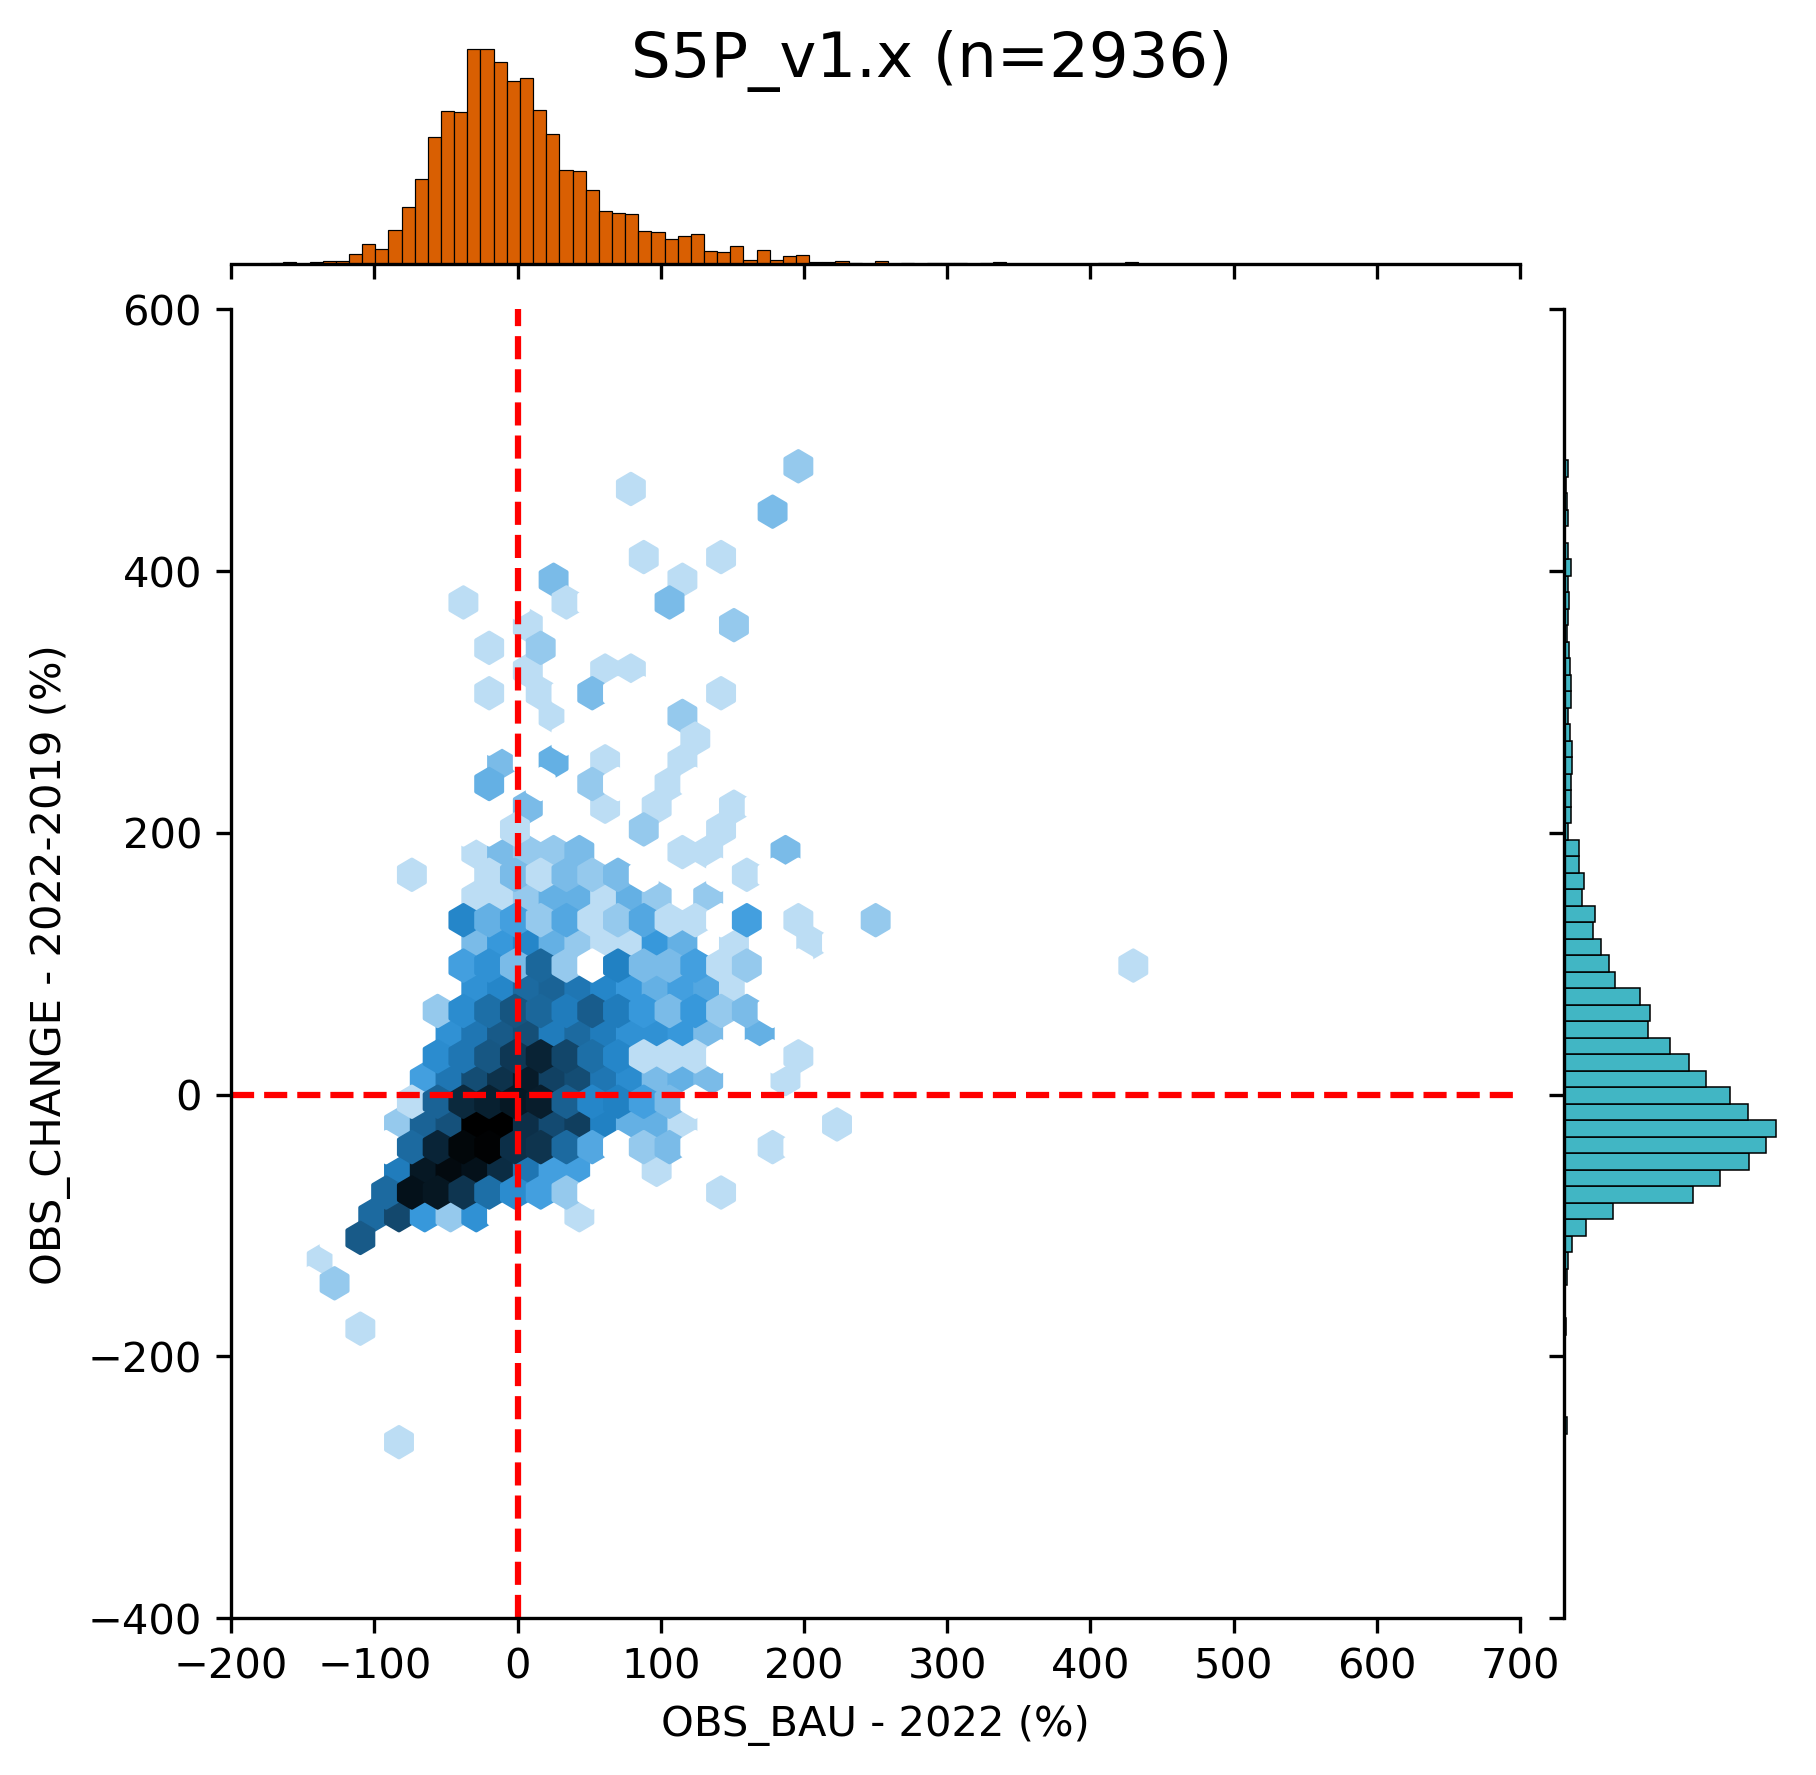
\includegraphics[width=\textwidth]{figs/chap3/fig7_a.png}
      \caption{}
      \label{fig:fig7a}
    \end{subfigure}%
    \begin{subfigure}{.5\textwidth}
      \centering
      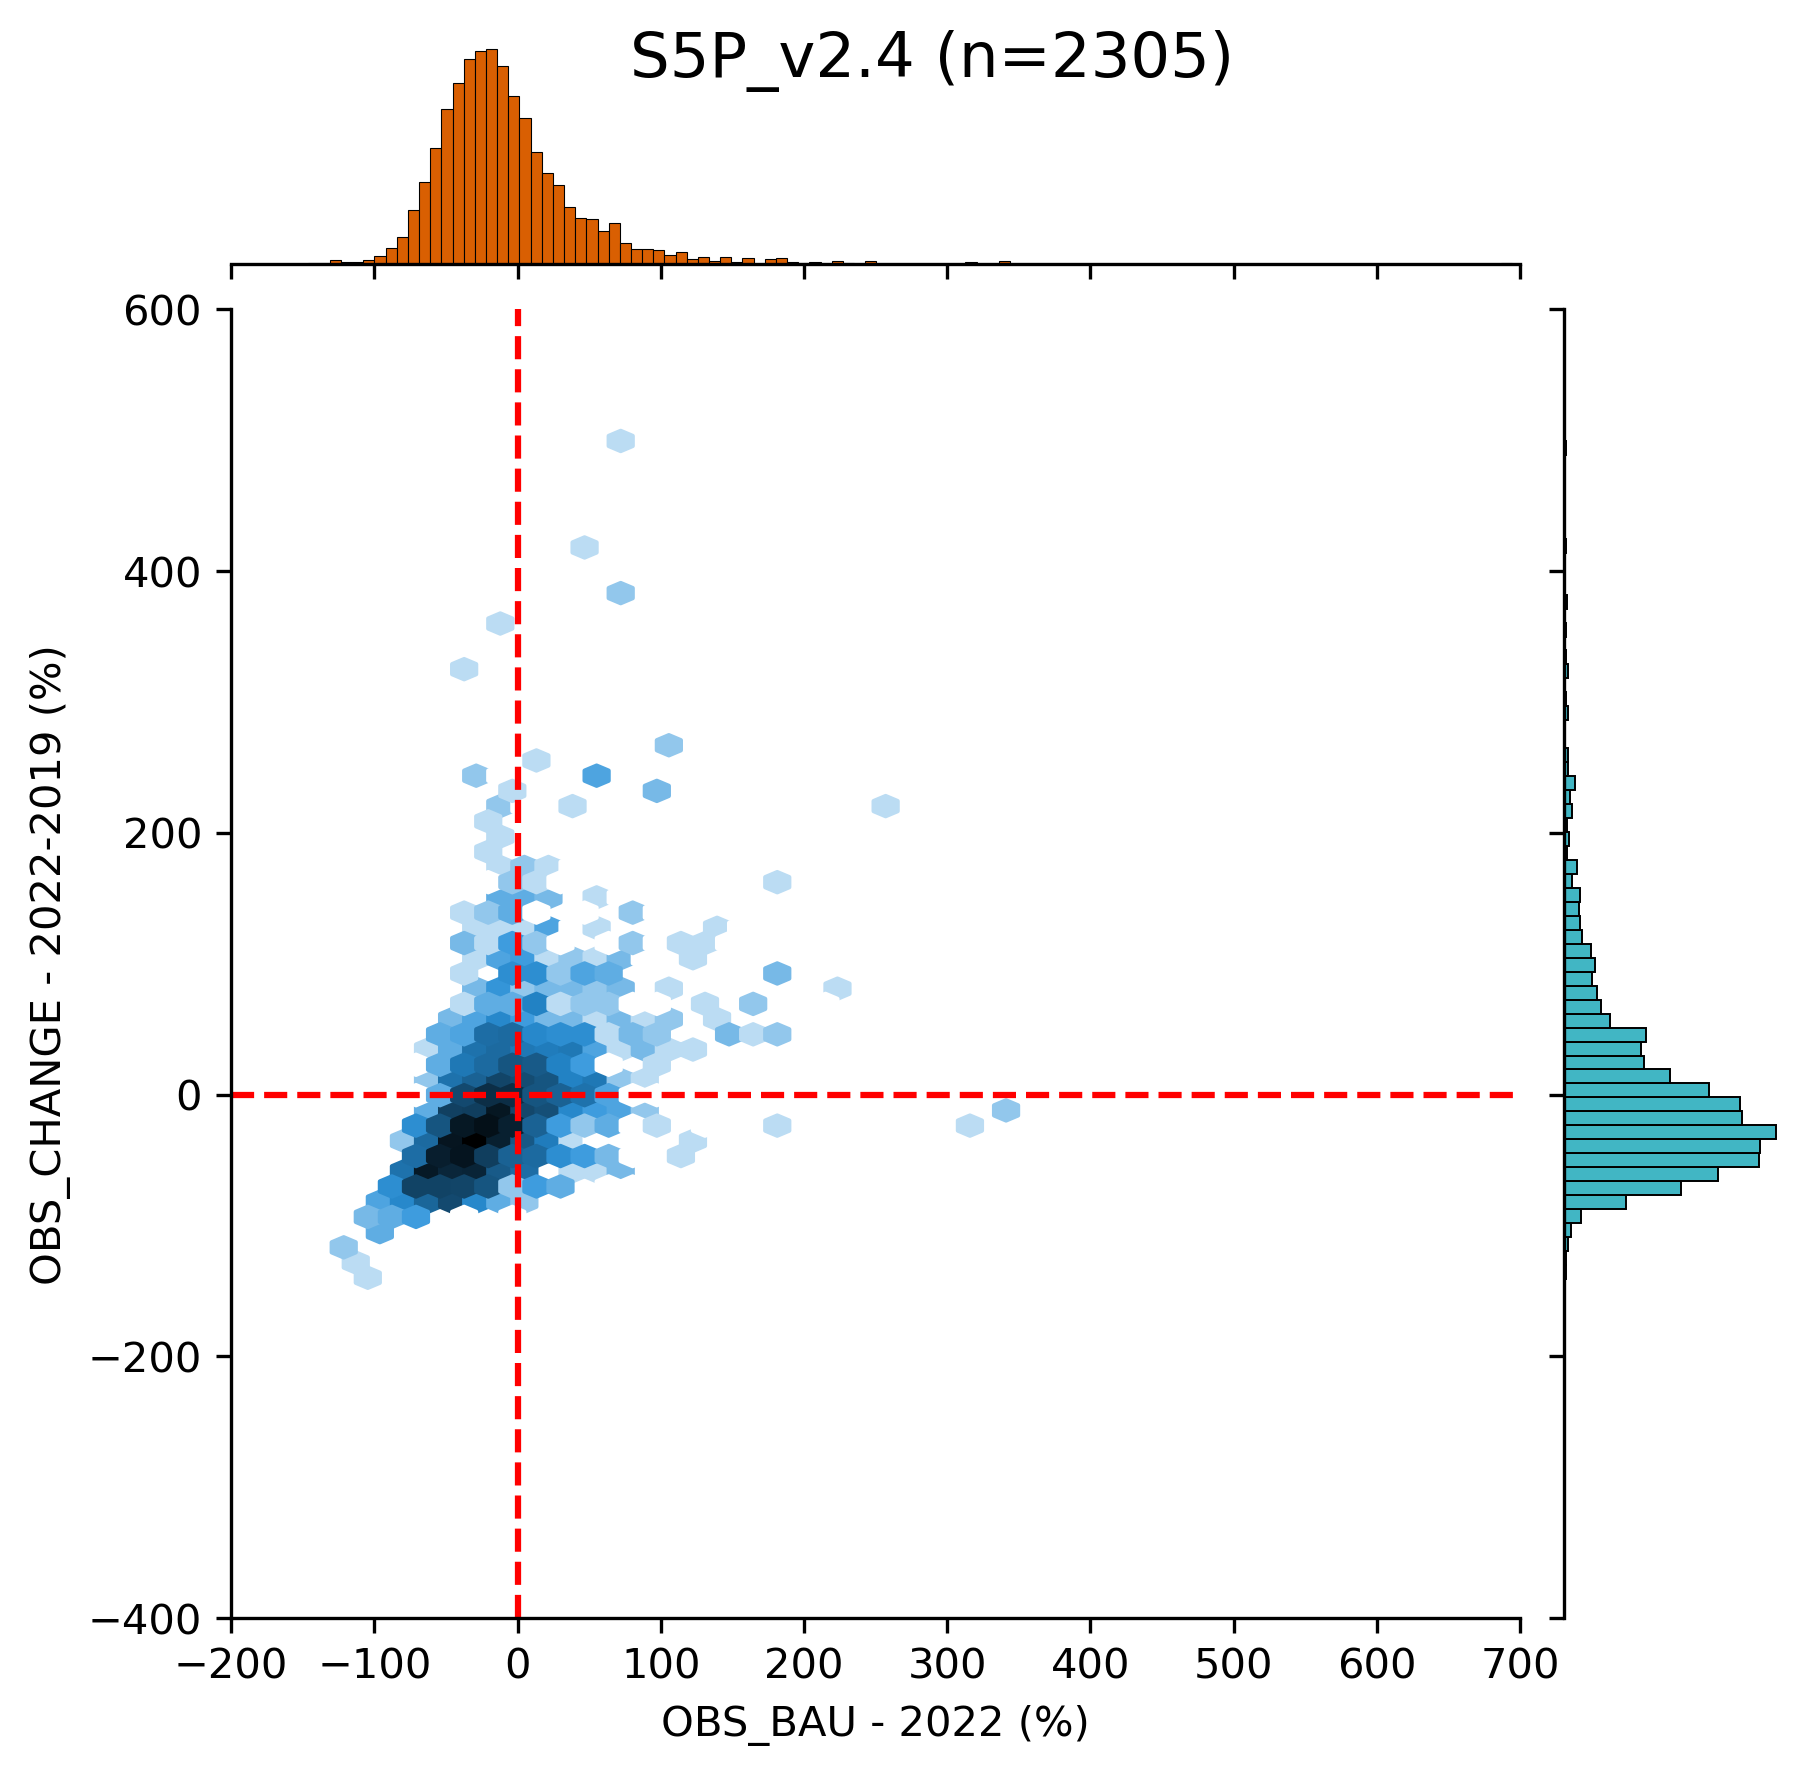
\includegraphics[width=\textwidth]{figs/chap3/fig7_b.png}
      \caption{}
      \label{fig:fig7b}
    \end{subfigure}
    \caption[NO2 level changes estimates for conflict events]{OBS-BAU and year-to-year estimates for the individual conflict events including air/drone strikes, armed clashes, remote explosive/landmine occurrences, shelling/artillery/missile attacks, and other forms of attacks that occurred between February 24 and July 31, 2022, for five frontline oblasts, Dnipropetrovsk, Donetsk, Kharkiv, Luhansk and Zaporizhzhia. The number of data points is denoted by (n).}
    \label{fig:chap3_fig7}
\end{figure}
The OBS-BAU estimates based on ORG data indicate an average increase of 0.3\%, while the year-to-year estimates show a more substantial increase of 13.2\%. However, when using RPRO data, we observed an 11\% reduction in the OBS-BAU estimate and a 1.35\% increase in the year-to-year estimate. Although there is a high level of uncertainty in estimating changes at the event location-pixel level, and the inconsistent timing between the reported conflict related events and S5P overpass may lead to an underestimation of changes in air pollution levels, the information gathered can still be useful in identifying changes in the NO2 columns associated with conflict related event locations in the five oblasts.\par
\subsection{Changes of S5P NO2 levels in other affected areas}
\subsubsection*{Most populous cities of Ukraine}
In the nine most populous cities in Ukraine, both the lockdown and the conflict have led to a reduction in daily anthropogenic activities. Although this reduction was expected to lower the NO2 levels, as discussed in Section 4, the lockdown measures did not result in a significant reduction in NO2 column levels in 2020. To quantify the changes caused by the conflict and compare them with the effects of the lockdown measures, we analysed the OBS-BAU estimate for the most populous cities in Ukraine during the strict lockdown period from April 6 to May 10 in 2020 and 2022 (Table \ref{tab:chap3_tab3}). To avoid overwhelming plots, Figure \ref{fig:chap3_fig8} displays the NO2 column trend lines for OBS data and BAU predictions from February to July in 2020 and 2022 for five cities (Kyiv, Kharkiv, Dnipro, Zaporizhzhia, and Kryvyi Rih) only.\par
\begin{figure}[p]
    \centering
    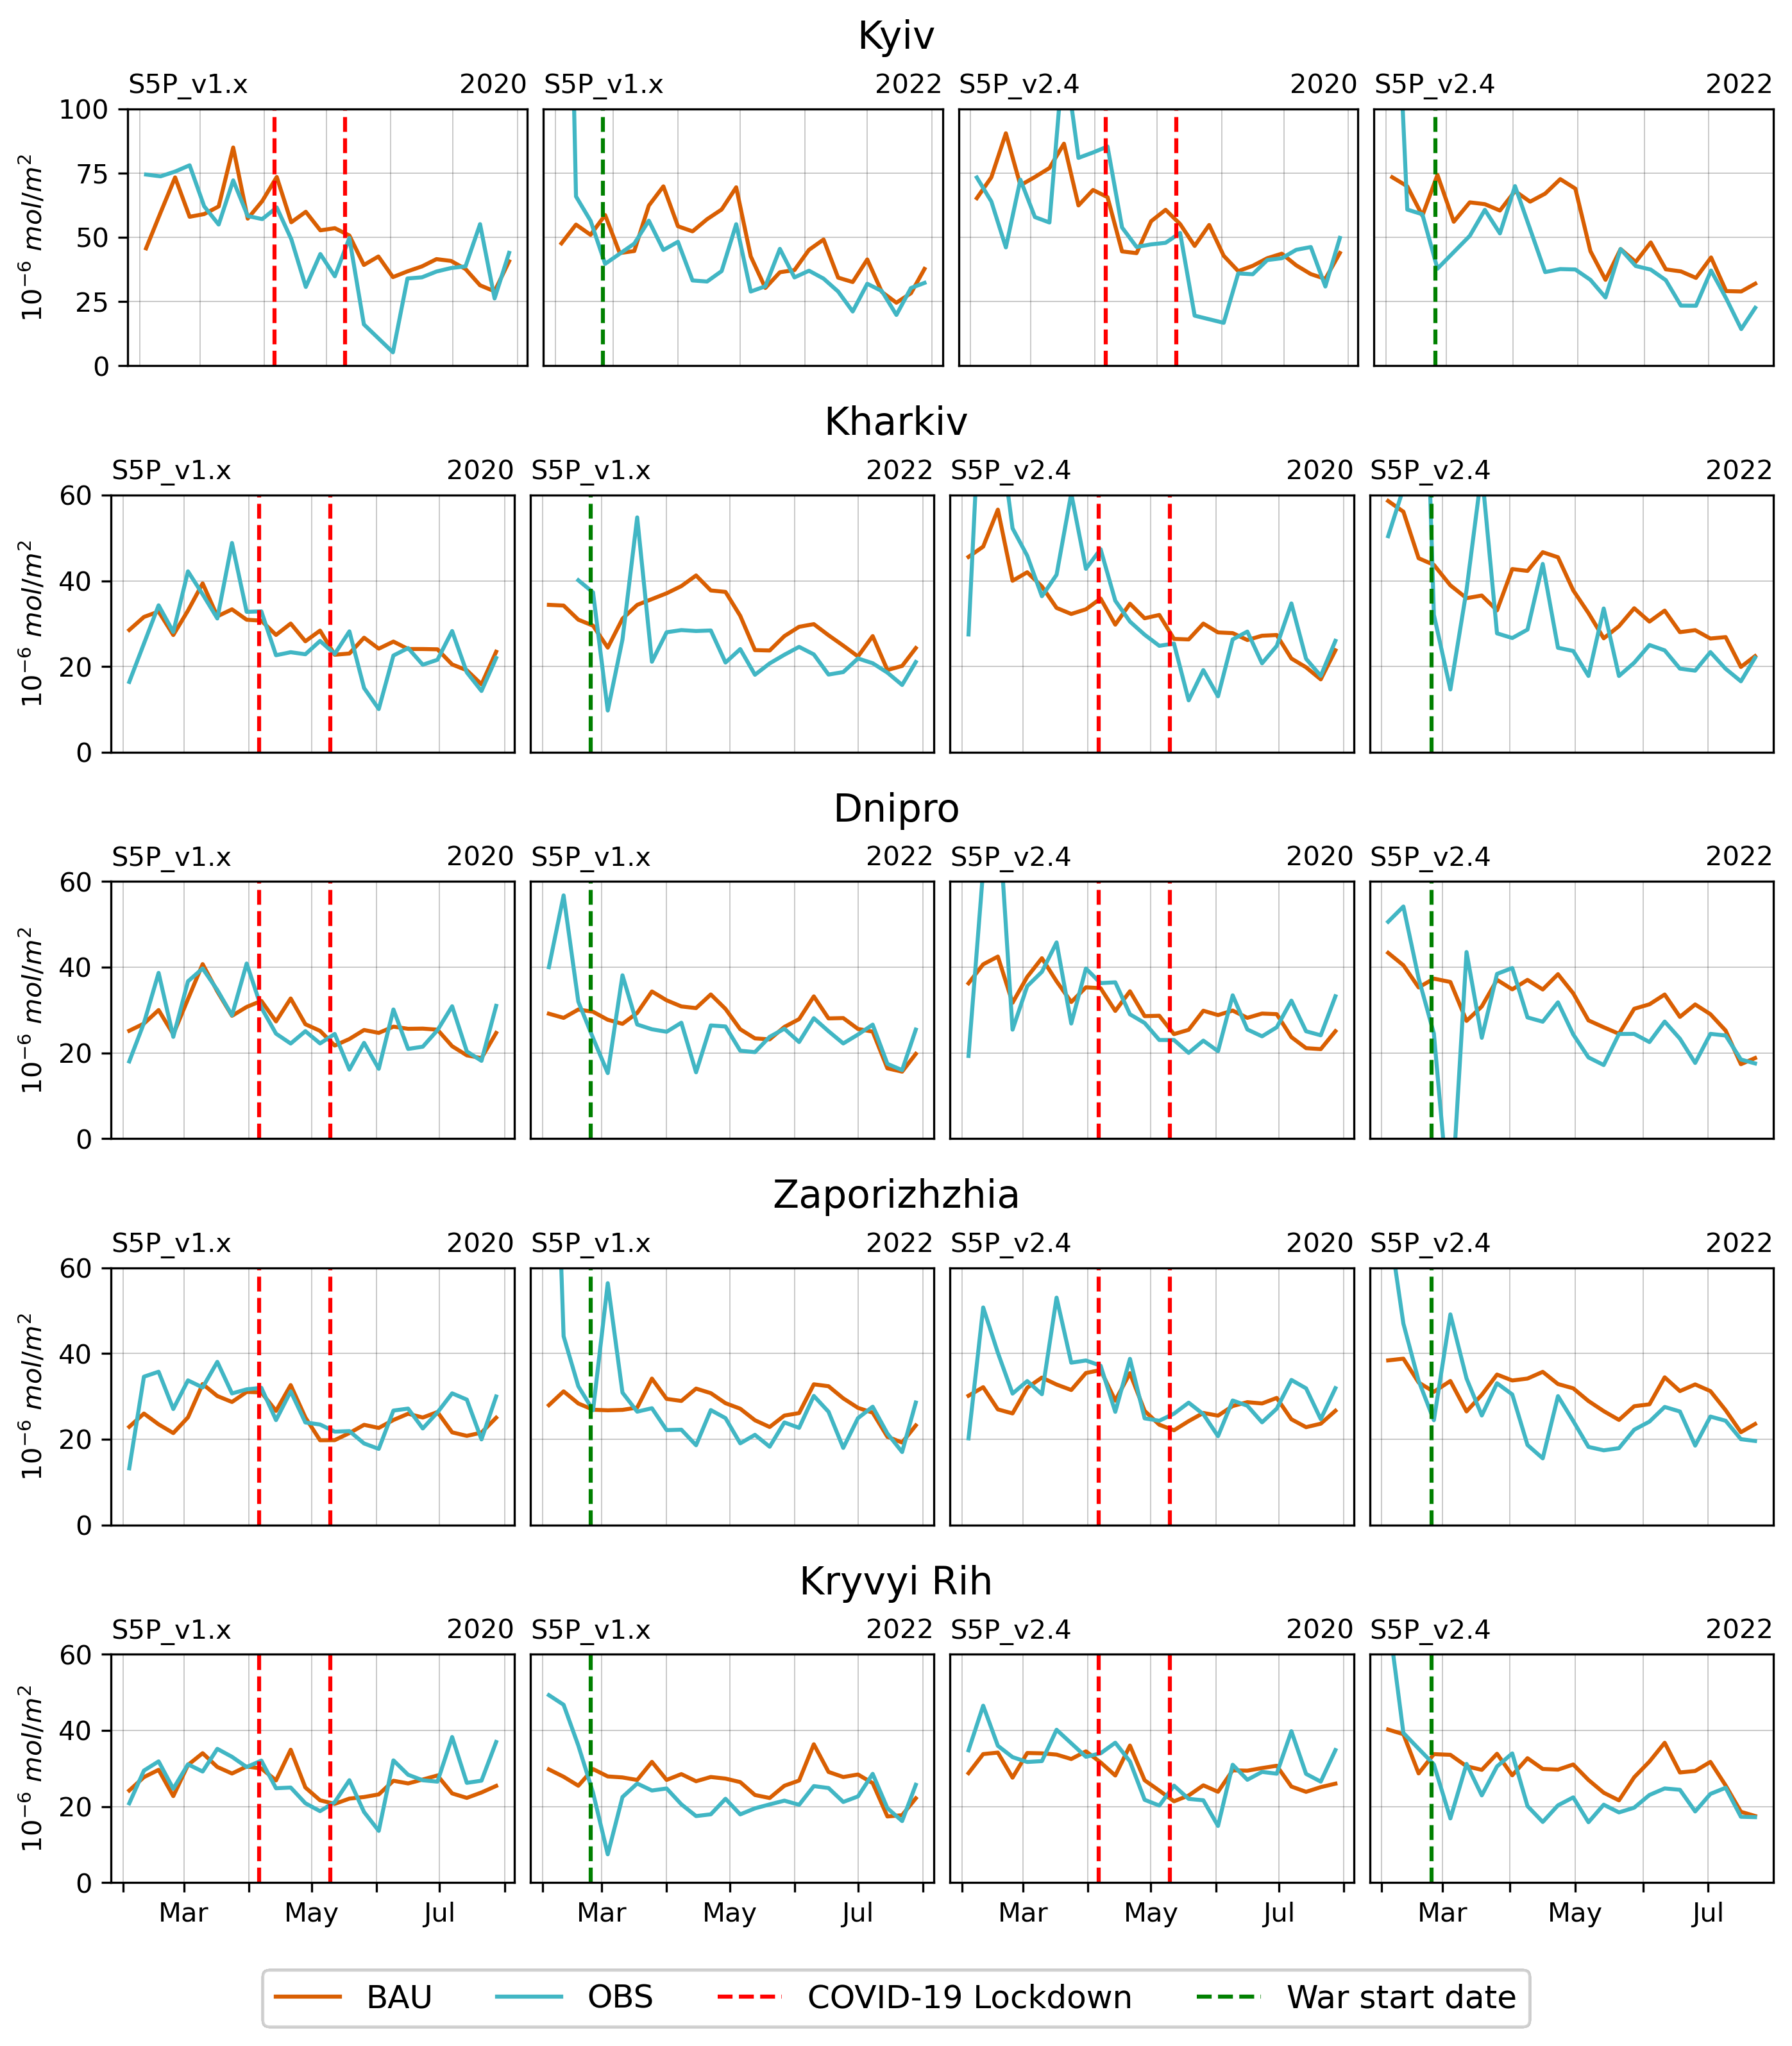
\includegraphics[width=\textwidth]{figs/chap3/fig8.png}
    \caption[OBS and BAU S5P NO2 trends (2020-2022) in populous cities]{The trend lines of OBS and BAU S5P NO2 column levels from February to July in 2020 and 2022 for five cities in Ukraine. Each row displays plots for a different city. The first and second column plots represent the ORG data (S5P version 1.x), while the third and last column plots show the RPRO data (S5P version 2.4). The first and third column plots pertain to 2020, while the second and last column plots pertain to 2022.}
    \label{fig:chap3_fig8}
\end{figure}


\begin{table}[!ht]
    \centering
    \caption[Comparison of NO2 changes during 2020 and 2022 lockdown period]{The OBS-BAU estimate (in percentage) of ORG data and RPRO data for the strict lockdown period (April 6 to May 10) in 2020 and in 2022 for the nine most populous cities in Ukraine. The values are represented as mean (with standard deviation in parentheses). The mean and standard deviation in the last row were calculated across the nine cities.}
    \begin{tabular}{c c c c c }
        \hline
            \multirow{2}{*}{City} & \multicolumn{2}{c}{2020 (April 6 \textminus May 10)} & \multicolumn{2}{c}{2022 (April 6 \textminus May 10)} \\ \cline{2-5}
            & {ORG} & {RPRO} & {ORG} & {RPRO} \\ \hline
            Kyiv & \textminus18.8 (6.5) & 4.9 (17.4) & \textminus29.3 (9.5) & \textminus34.6 (7.6)  \\
            Kharkiv & \textminus0.9 (10.3) & \textminus4.9 (15.9) & \textminus24.9 (17.9) & \textminus29.7 (20.8)  \\
            Odessa & 6.9 (12.4) & 21.0 (16.4) & \textminus7.6 (14.3) & \textminus14.5 (9.7)  \\
            Dnipro & \textminus6.6 (9.2) & 2.8 (10.9) & \textminus17.4 (10.0) & \textminus19.5 (8.6)  \\
            Donetsk & 28.2 (35.2) & 42.0 (29.8) & 3.5 (19.9) & 3.2 (18.7)  \\
            Zaporizhzhia & 2.5 (9.1) & 9.1 (12.7) & \textminus12.6 (13.7) & \textminus18.4 (11.6)  \\
            Lviv & 0.0 (10.9) & 3.0 (8.5) & 14.9 (17.9) & \textminus3.3 (9.9)  \\
            Kryvyi Rih & \textminus6.4 (8.7) & 0.1 (9.9) & \textminus20.8 (9.8) & \textminus27.7 (8.1)  \\
            Mykolaiv & \textminus0.6 (9.8) & 13.8 (17.6) & \textminus14.6 (10.1) & \textminus18.0 (6.8)  \\
            Mean & 0.5 (11.9) & 10.2 (13.3) & \textminus12.1 (13.2) & \textminus18.1 (11.5) \\ \hline
    \end{tabular}
    \label{tab:chap3_tab3}
\end{table}

\begin{table}[!ht]
    \centering
    \caption[S5P NO2 variations in populous cities from February to July 2022]{Average OBS-BAU and year-to-year estimate (in percentage) of ORG data and RPRO data from February 24 to July 31, 2022, for the nine most populous cities in Ukraine. The values are represented as mean (with standard deviation in parentheses). The mean and standard deviation in the last row were calculated across the nine cities.}
    \begin{tabular}{c c c c c }
        \hline
            \multirow{2}{*}{City} & \multicolumn{2}{c}{ORG} & \multicolumn{2}{c}{RPRO} \\\cline{2-5}
            & {OBS-BAU} & {year-to-year} & {OBS-BAU} & {year-to-year} \\ \hline
            Kyiv & \textminus14.9 (17.3) & \textminus30.5 (14.7) & \textminus27.6 (12.1) & \textminus37.3 (11.3)  \\
            Kharkiv & \textminus3.2 (28.5) & 20.7 (39.8) & \textminus3.0 (33.3) & 2.4 (23.6)  \\
            Odessa & \textminus6.8 (15.4) & \textminus13.6 (16.4) & \textminus5.4 (13.0) & 4.5 (61.0)  \\
            Dnipro & \textminus12.4 (16.6) & \textminus15.0 (21.3) & \textminus17.6 (13.8) & \textminus17.0 (20.5)  \\
            Donetsk & 19.4 (26.6) & 4.2 (21.5) & 17.0 (22.8) & \textminus9.4 (15.8)  \\
            Zaporizhzhia & \textminus10.5 (16.4) & \textminus15.7 (27.3) & \textminus13.7 (14.4) & \textminus19.1 (18.6)  \\
            Lviv & 20.8 (21.9) & \textminus9.0 (24.1) & 2.2 (16.8) & \textminus9.8 (17.3)  \\
            Kryvyi Rih & \textminus15.5 (15.7) & \textminus22.4 (21.7) & \textminus17.4 (15.0) & \textminus26.2 (42.7)  \\
            Mykolaiv & \textminus4.8 (13.1) & \textminus7.8 (23.5) & 2.1 (14.8) & 12.9 (21.9)  \\
            Mean & \textminus3.1 (13) & \textminus9.9 (14.1) & \textminus7 (12.7) & \textminus11 (15) \\ \hline
    \end{tabular}
    \label{tab:chap3_tab4}
\end{table}

Table \ref{tab:chap3_tab3} presents the OBS-BAU estimates corresponding to the strict lockdown period (April 6 to May 10) in 2020 and 2022 for the nine most populous cities in Ukraine. Our findings indicate that the conflict has caused more significant reductions in NO2 levels, compared to the lockdown measures. While minor reductions to increases were observed during the 2020 lockdown, a consistent and continuous reduction has been noticed in most cities, during the same lockdown period (April 6 to May 10) in 2022. The average reduction across all the cities of interest, as shown in Table \ref{tab:chap3_tab3}, is about 12.1\% (based on ORG data) and 18.1\% (based on RPRO data). The largest reduction was observed in Kyiv, while the increase occurred in Lviv (14.9\% based on ORG data) and in Donetsk (3.5\% based on ORG data, 3.2\% based on RPRO data).\par

In more than the first five months after the conflict began until the end of July 2022, an overall reduction is observed across the nine cities (see Table \ref{tab:chap3_tab4}) with an average of 3.1\% (ORG data) and 7\% (RPRO data). The largest reductions in NO2 levels were observed in Kyiv, with an average of 14.9\% (ORG data) and 27.6\% (RPRO data). Conversely, Donetsk and Lviv experienced increases in NO2 levels, with both ORG and RPRO data, while in Mykolaiv only RPRO data showed the increases. The rise in Donetsk can be attributed to it being where major armed conflicts occurred during this period.\par
\subsubsection*{Coal power plants}
Besides anthropogenic activities in major cities, the contribution of CPPs to NO2 concentration levels is considered to be significant in Ukraine \citep{lauri2021}. The Zaporizhzhia CPP is one of the largest emitters among CPPs in Ukraine, emitting 21,830 tonnes of NOx in 2019. Many power plants have been targeted in the conflict, and their damage or destruction has resulted in power blackouts affecting millions of people. \par

\begin{figure}[p]
    \centering
    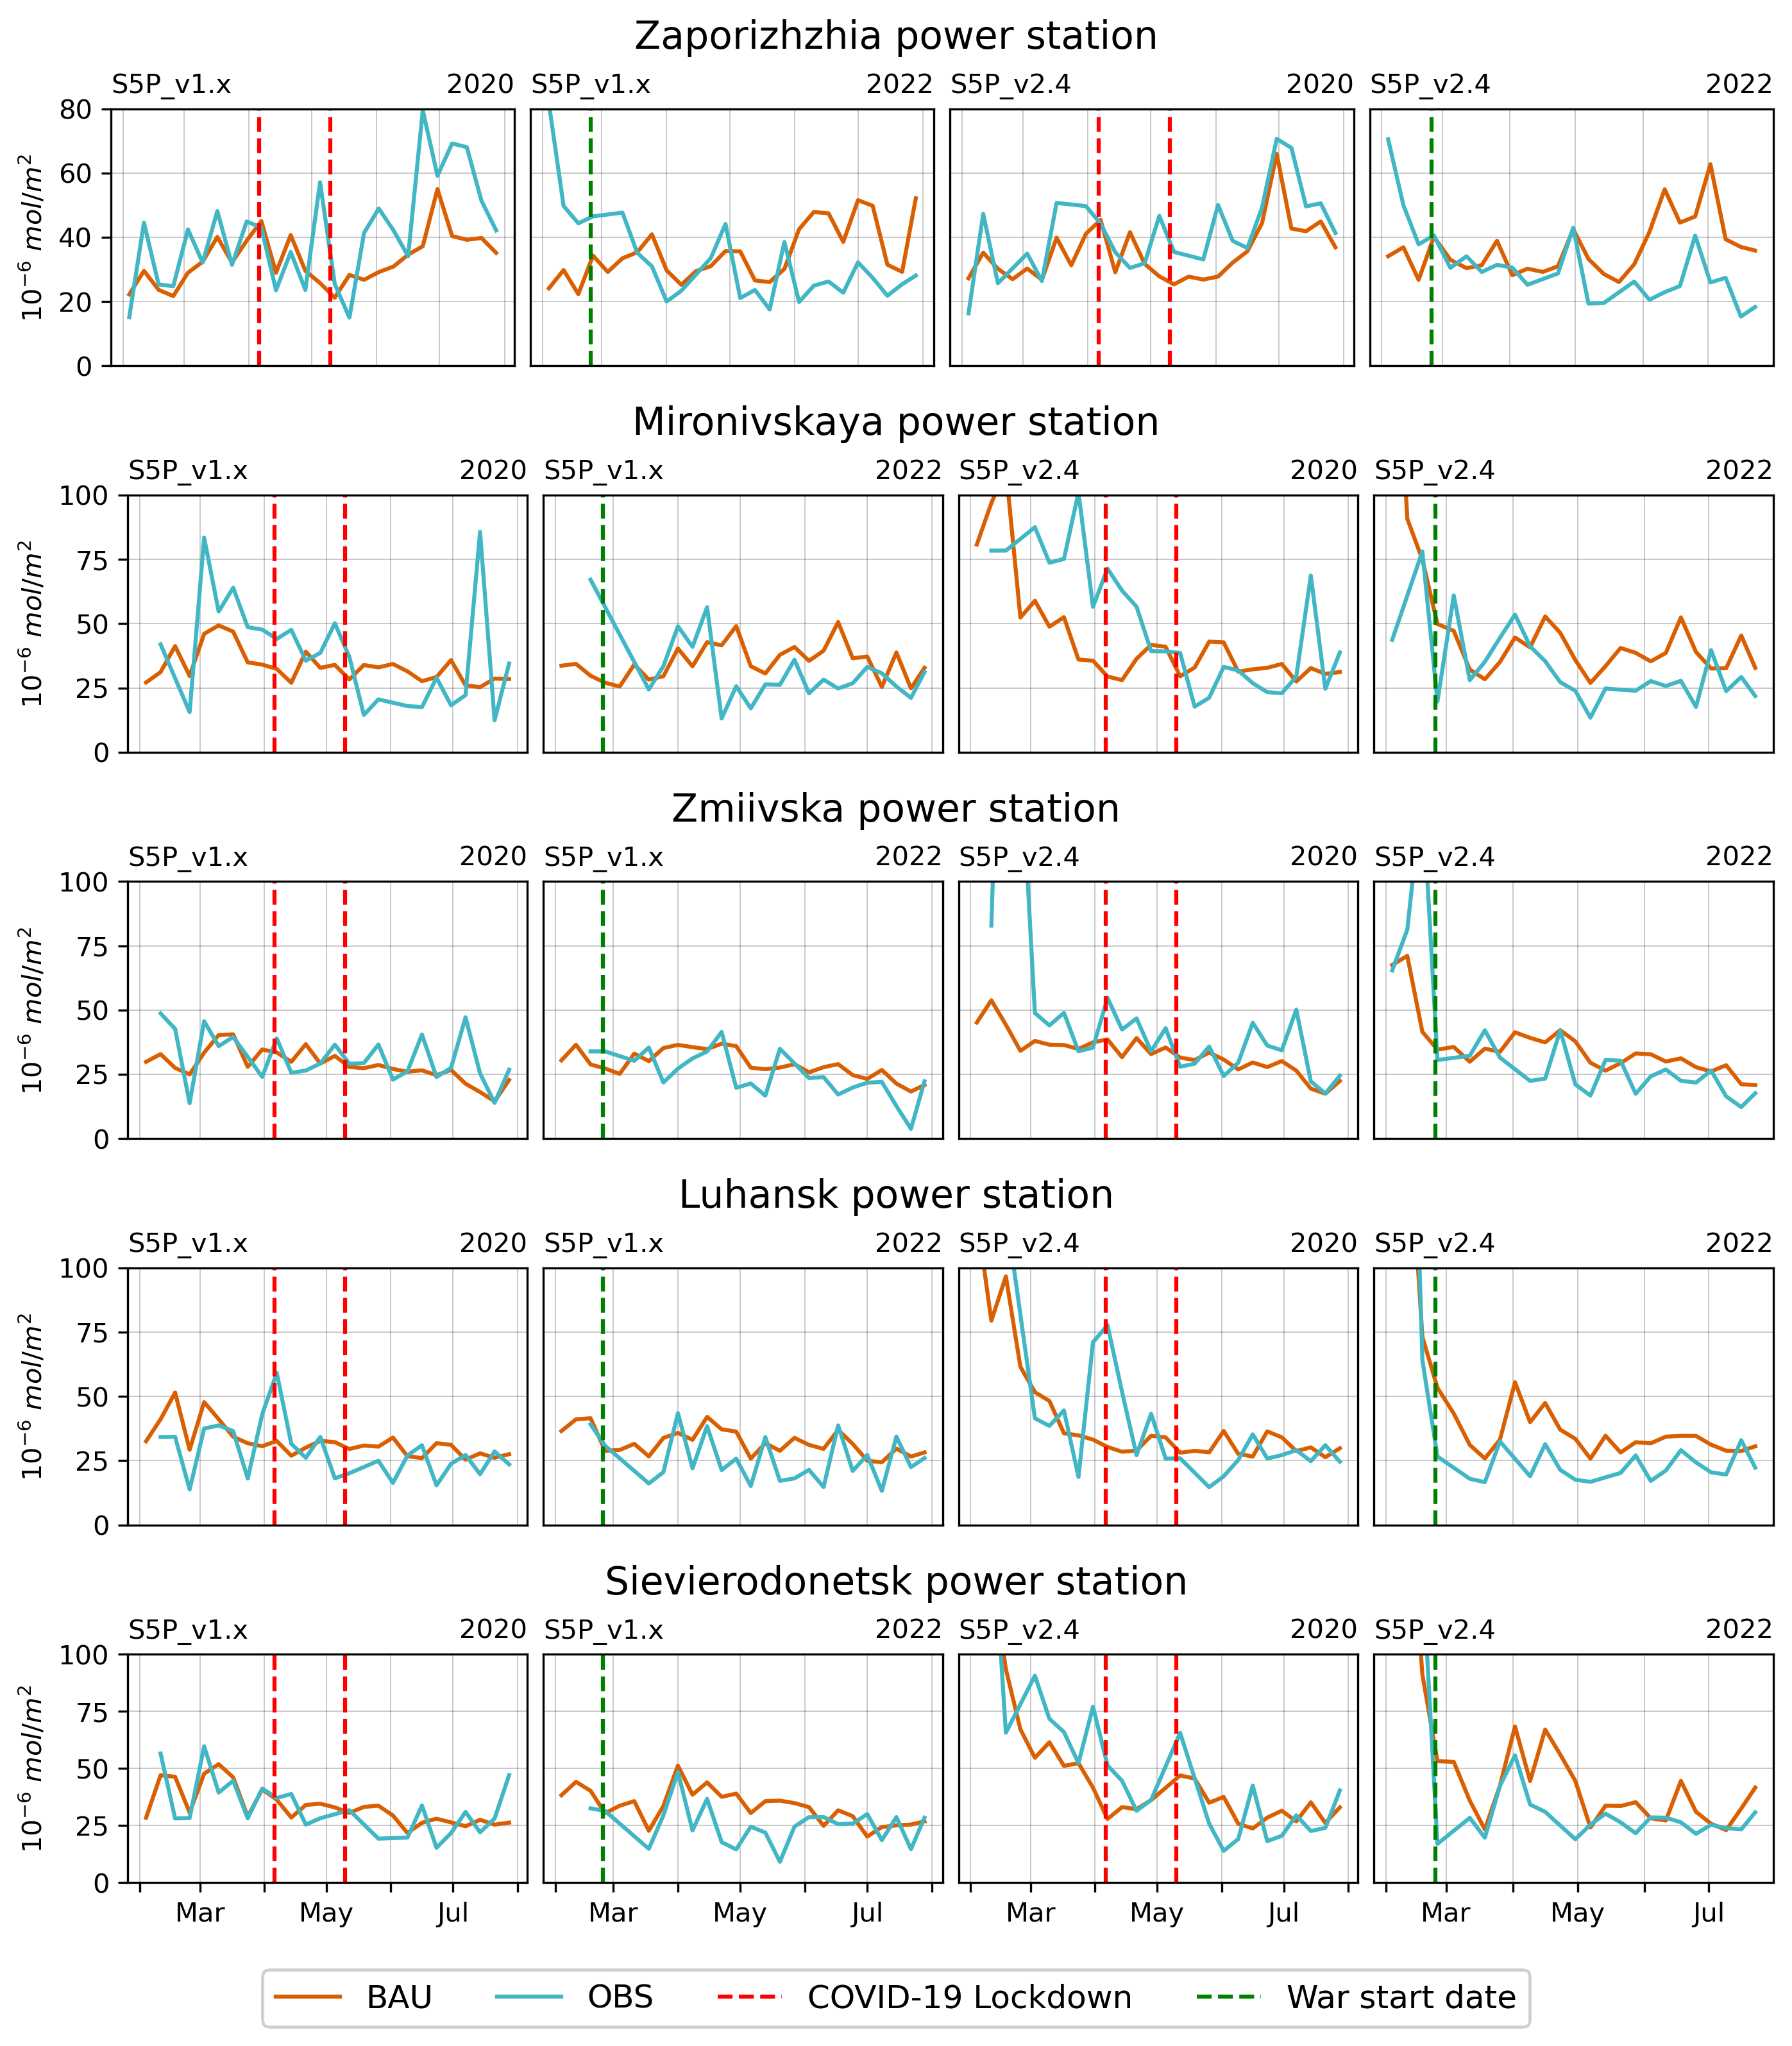
\includegraphics[width=\textwidth]{figs/chap3/fig9.png}
    \caption[OBS and BAU S5P NO2 trends (2020-2022) for selected CPPs]{The trend lines for the OBS and BAU S5P NO2 column levels from February to July in 2020 and 2022 are presented for selected CPPs. Each row displays plots for a different CPP. The first and second column plots represent ORG data (S5P version 1.x), while the third and last column plots show RPRO data (S5P version 2.4). The first and third column plots pertain to 2020, while the second and last column plots pertain to 2022.}
    \label{fig:chap3_fig9}
\end{figure}

According to Draft Ukraine Recovery Plan, Materials of the “Energy Security” Working Group covering the period to the end of June 2022, significant damage has been reported at the Zaporizhzhia, Luhansk, and Sievierodonetsk power stations, as well as other CPPs. This damage could be expected to affect NO2 levels in the areas surrounding the damaged power plants. To investigate such changes, we also compare trends in the NO2 column levels between OBS data and BAU simulations for 2020 and 2022, utilizing both ORG and RPRO data as presented in Figure \ref{fig:chap3_fig9}. Examining an area of 10km2 around each CPP, we find that, similar to previous discussions on lockdown effects, little changes are observed around most CPPs during the pandemic lockdown in 2020. However, a clear reduction is evident between the time when the conflict began and July 2022 at the Zaporizhzhia, Mironivskaya, Zmiivska, Luhansk, and Sievierodonetsk power stations. At areas surrounding other power stations, no noticeable reduction is observed.\par

\section{Conclusion} \label{chap3_conclusion}
In this study, we performed a comprehensive assessment of variations in the S5P column NO2 levels in Ukraine during the COVID-19 pandemic lockdown in 2020 and the armed conflict with Russia in 2022. For this purpose, we utilized two S5P products, namely, original and reprocessing data. We first developed a weather normalization model under business-as-usual conditions, using meteorological parameters from ERA5 reanalysis, ensembled surface forecasts, and analysis NO2 data from 11 CAMS models, along with other spatial and temporal features. Next, we applied the BAU prediction to estimate the change in NO2 levels during the lockdown period in 2020 for the nine most populous cities in Ukraine (Kyiv, Kharkiv, Odessa, Dnipro, Donetsk, Zaporizhzhia, Lviv, Kryvyi Rih, and Mykolaiv). We extended the analysis using BAU predictions to estimate the impact of the armed conflict from February 24 to July 31, 2022, in conflict hotspot locations, the nine most populous cities, and areas surrounding selected CPPs (Zaporizhzhia, Mironivskaya, Zmiivska, Luhansk, and Sievierodonetsk) in Ukraine.\par

The main outcomes of the study can be summarized as follows:\par
\begin{itemize}
    \item In 2020, meteorological parameters also heavily influenced the NO2 tropospheric column levels, contributing to decreases in levels during the lockdown period.
    \item After normalizing the meteorological parameters, we found that the lockdown did not lead to lower NO2 levels than the BAU prediction in 2020, although it did manage to mitigate the increase in NO2 compared to the pre-lockdown period. Our study indicates that stricter measures may need to be considered in the future to achieve a significant reduction in NO2 levels in densely populated areas of Ukraine.
    \item We observed that satellite-capture fire data from the VIIRS product can capture the spatial patterns of the conflict related events on the ground. From this product, conflict location patterns are clearly represented during the April–July 2022 period.
    \item Upon examining changes in NO2 levels at conflict hotspots at the location-pixel level, we observed changes ranging from an 11\% reduction to a slight increase of 0.3\% when comparing the OBS to BAU predictions using RPRO and ORG data, respectively.
    \item During the strict lockdown period from April 6 to May 10, 2022, the reduction in NO2 levels in the nine most populous cities was more significant compared to 2020. Across most cities, an average reduction of 12.1\% (ORG data) and 18.1\% (RPRO data) was observed. However, it is worth noting that Lviv and Donetsk showed an increase in NO2 levels during this period.
    \item From February 24 to July 31, 2022, the nine most populous cities in Ukraine experienced an overall reduction of 3.1\% (ORG data) and 7\% (RPRO data) in NO2 levels. The most significant reduction was observed in Kyiv, with an average decrease of 14.9\% (ORG data) and 27.6\% (RPRO data). However, in contrast, NO2 levels increased in Lviv, Donetsk and Mykolaiv during this period.
    \item The conflict has resulted in damage to several CPPs, which are considered as major sources of NO2 emissions in the country. Our analysis indicates a clear reduction in NO2 levels in the areas closely surrounding Zaporizhzhia, Mironivskaya, Zmiivska, Luhansk, Sievierodonetsk CPPs.
    \item By utilizing the OBS-BAU estimate for both ORG data and RPRO data to analyse NO2 variations during the 2022 conflict, we found that discrepancies resulting from changes in the processor during the S5P lifetime in ORG data might lead to a slight underestimation of NO2 reductions. Specifically, we observed a smaller decrease using ORG data (3.1\%) than with RPRO data (7\%) in the most populous cities of Ukraine.
\end{itemize}

The consideration of meteorological effects is crucial in regulating pollution levels. Neglecting these effects could introduce errors in quantifying actual air quality changes attributed to an intervention event. For future studies assessing the impacts of conflict in Ukraine on air quality, it will be essential to account for meteorological variability to achieve genuine and quantitative estimates.\par

NO2 is a significant precursor to tropospheric O3 and also affects the lifetime of methane (CH4) \citep{akimoto2022rethinking}. Additionally, it has the potential to serve as an indicator for monitoring CO2 emissions \citep{miyazaki2023predictability}. In future studies, it would be valuable to explore how changes in NO2 levels during conflict could impact O3 and CH4 concentrations in Ukraine as both are important short-lived climate pollutants that contribute to positive radiative forcing, thereby exacerbating global warming.\par
